\documentclass[a4paper,12pt,oneside]{report}
\usepackage[english]{../../../../latex-setup/learningnotes}
\usepackage{needspace}
\usepackage{pgfplots}
\usetikzlibrary{decorations.pathreplacing}
\pgfplotsset{compat=1.18}
\hypersetup{linktoc=all}
\setcounter{secnumdepth}{3}

\newcommand{\exerciseheading}[1]{%
  \par\Needspace{5\baselineskip}\noindent\textbf{#1}\par\nobreak}
\newcommand{\solutionheading}[1]{%
  \par\Needspace{5\baselineskip}\noindent
  \begingroup\setlength{\fboxsep}{1pt}%
  \colorbox{yellow}{\strut\textbf{#1}}\endgroup\par\nobreak}

% Computational problems are stated in definition-coloured boxes.
\newtcolorbox{framedproblem}[1]{definitionbox,title={Problem:\enspace #1}}
\newcommand{\ED}{\operatorname{ED}}
\newcommand{\LCS}{\operatorname{LCS}}
\newcommand{\OPT}{\mathrm{OPT}}

% Line colours for plots, checked for colour-vision deficiencies.
\definecolor{PlotRed}{HTML}{C0392B}
\definecolor{PlotBlue}{HTML}{2F5BD3}
\definecolor{PlotGreen}{HTML}{2E8B3E}

% Coloured underline: tracks which term becomes what in an expansion.
\newcommand{\cul}[2]{%
  \tikz[baseline=(cul.base)]{%
    \node[inner sep=0pt,outer sep=0pt] (cul) {$\displaystyle #2$};
    \draw[#1,line width=1.2pt]
      ([yshift=-2.5pt]cul.south west) -- ([yshift=-2.5pt]cul.south east);}}

% Keep each list operation's underline consistent across implementations.
\definecolor{ListGet}{HTML}{0072B2}
\definecolor{ListSet}{HTML}{D55E00}
\definecolor{ListInsert}{HTML}{009E73}
\definecolor{ListRemove}{HTML}{AA4499}
\newcommand{\listgetop}[1]{\cul{ListGet}{\operatorname{get}(#1)}}
\newcommand{\listsetop}[2]{\cul{ListSet}{\operatorname{set}(#1,#2)}}
\newcommand{\listinsertop}[2]{\cul{ListInsert}{\operatorname{insert}(#1,#2)}}
\newcommand{\listremoveop}[1]{\cul{ListRemove}{\operatorname{remove}(#1)}}
% Priority queues reuse the insertion, reading and removal colours.
\newcommand{\pqinsertop}[1]{\cul{ListInsert}{\operatorname{insert}(#1)}}
\newcommand{\pqpeekop}[1]{\cul{ListGet}{\operatorname{peek#1}()}}
\newcommand{\pqextractop}[1]{\cul{ListRemove}{\operatorname{extract#1}()}}

% Yellow lecture banner, as in the FSL notes before the chapter reorganization.
\newcommand{\lecturebanner}[1]{%
  \Needspace{6\baselineskip}%
  \begin{tcolorbox}[colback=yellow!20,colframe=yellow!60!black,
    boxrule=0.4pt,arc=1mm,left=5pt,right=5pt,top=3pt,bottom=3pt,
    before skip=6pt,after skip=6pt]
  \small\textbf{#1}
  \end{tcolorbox}}
\newcommand{\lecturestart}[1]{\lecturebanner{Start of lecture #1}}

\notestitle{ADM}
\notessubtitle{Algorithmic Methods of Data Mining}
\notesauthor{Matteo}
\notesdate{\today}

\begin{document}

\makenotestitle

\thispagestyle{empty}
\begin{tcolorbox}[
  examplebox,unbreakable,title={Acknowledgements},
  colframe=blue!35!black,coltitle=white,
  arc=5mm,outer arc=5mm,left=3mm,right=3mm,top=3mm,bottom=3mm,
  boxed title style={
    colback=blue!35!black,colframe=blue!35!black,
    arc=3mm,outer arc=3mm,
    frame code={
      \path[fill=tcbcolframe,draw=tcbcolframe,rounded corners=3mm]
        (frame.south west) rectangle (frame.north east);
    }}]
Thanks to \href{https://github.com/flaviac18-hub}{Flavia} for sharing
her handwritten notes for Algorithmic Methods of Data Mining,
which made this document possible.
\end{tcolorbox}
\clearpage

\notescontents

\chapter{Introduction to data mining}

\lecturestart{24 September}

\section{Course organization}

The course has two parts. The first part brings everyone to the same
level, especially those who have not studied computer science before:
basic computer architecture, data structures (different problems call
for different ways of storing data), algorithms (how to solve a problem
quickly, or even optimally, and how to measure its complexity), and
programming, practised in the lab, in the homeworks and in the
hackathon. The second part covers data mining topics: text mining,
clustering and graphs.

\section{What is data mining?}

Huge amounts of data are produced in every field: social networks,
for instance, both contain and generate an enormous quantity of data.
These data hide patterns that we would like to find, but the amount is
far too large to inspect by hand. Data mining tools let us explore
data that we could not otherwise process.

\begin{frameddefn}{Data mining}\label{def:data-mining}
\emph{Data mining} is the use of efficient techniques for the analysis
of very large collections of data and the extraction of useful and
possibly unexpected patterns in data.
\end{frameddefn}

We will meet two kinds of tasks:
\begin{itemize}
  \item \textbf{Descriptive tasks} summarize the data and reveal their
    structure, for example groups of similar objects.
  \item \textbf{Predictive tasks} use the data to predict something
    unknown, for example whether a person will click on an advertisement.
\end{itemize}

\section{Structured, unstructured and semi-structured data}

Data come with different amounts of organization.

\begin{frameddefn}{Structured, unstructured and semi-structured data}
\label{def:data-structure-levels}
\begin{itemize}
  \item \emph{Structured data} have a clean, fixed form. For example,
    a university's student records store a name, a surname and a
    student ID for every student. These are the best data we can hope
    for.
  \item \emph{Unstructured data} have no predefined form, for example
    text and pages found on the internet. Most of the data we meet are
    of this kind.
  \item \emph{Semi-structured data} lie in between: they have some
    structure, but it can be modified freely. Spreadsheets (Excel) and
    XML files are typical examples.
\end{itemize}
\end{frameddefn}

\begin{notebox}[Data cleaning]
Data must be cleaned before they are analysed: if the data are dirty,
the algorithm will not work. Cleaning used to be very hard to do by
hand; today software tools help, but we should still check that the
result is correct. Semi-structured data are especially prone to errors,
because their structure is easy to break.
\end{notebox}

\lecturestart{28 September}

\section{Types of data}

Data are very heterogeneous. Common types include:
\begin{itemize}
  \item \textbf{Table (record) data}, such as spreadsheets; also images
    and time series.
  \item \textbf{Transaction data}: each record is a transaction between
    two parties, such as a credit-card payment or a shopping basket.
  \item \textbf{Document data}: Wikipedia pages, tweets, \ldots
  \item \textbf{Network data}: the web, where pages are linked to one
    another. Google works with these graphs, and Wikipedia's internal
    links form one as well.
  \item \textbf{Genomic sequences}: databases of DNA sequences, often
    used to find correlations with diseases.
  \item \textbf{Climate data}.
  \item \textbf{Behavioural data}: everything recorded about us, for
    example by smartphones.
\end{itemize}

\section{Data as mathematical objects}

\subsection{Records, attributes and sparsity}

In table data, each \emph{row} describes an object (for example a
person) and each \emph{column} describes an \emph{attribute} of the
object.

\begin{frameddefn}{Sparsity}\label{def:sparsity}
A data table is \emph{sparse} when most of its cells are empty (or
zero). The \emph{sparsity} of a table describes how many of its cells
are filled, that is, whether many or few values are missing.
\end{frameddefn}

Attributes can be of different types:
\begin{itemize}
  \item \textbf{Binary}: two possible values, such as yes/no.
  \item \textbf{Categorical}: values in a finite set of classes, such
    as a colour or a school grade like ``good'' or ``bad''.
  \item \textbf{Numeric}: numbers, either \emph{discrete} (counts) or
    \emph{continuous} (time, length, temperature).
\end{itemize}
We can also move between types: a numeric attribute can be turned into
a categorical one by grouping values into classes, and categories can
be encoded as numbers.

\subsection{Numeric records as points and vectors}

To analyse data with algorithms, we represent them as mathematical
objects. Suppose a table has $2000$ rows (people) and $7$ numeric
attributes. Each row is then an element of $\R^7$, which we can view
either as a \emph{point} in a $7$-dimensional space or as a
\emph{vector} starting from the origin.

\begin{center}
\begin{tikzpicture}[scale=0.95]
  \draw[->] (0,0) -- (2.7,0) node[right] {\small $x_1$};
  \draw[->] (0,0) -- (0,2.3) node[above] {\small $x_2$};
  \foreach \x/\y in {0.6/1.4,1.1/0.9,1.6/1.7,2.1/0.6,1.3/1.95}
    \fill[NotesBlue] (\x,\y) circle (1.7pt);
  \node at (1.3,-0.5) {\small rows as points};
  \begin{scope}[xshift=5cm]
    \draw[->] (0,0) -- (2.7,0) node[right] {\small $x_1$};
    \draw[->] (0,0) -- (0,2.3) node[above] {\small $x_2$};
    \foreach \x/\y in {0.6/1.4,1.1/0.9,1.6/1.7,2.1/0.6,1.3/1.95}
      \draw[->,thick,NotesBlue] (0,0) -- (\x,\y);
    \node at (1.3,-0.5) {\small rows as vectors};
  \end{scope}
\end{tikzpicture}
\end{center}

\subsection{Document data}

A text contains many words. We represent a document as a vector with
one dimension per word of the vocabulary; each entry counts how many
times that word appears in the document.

\begin{framedexample}{Documents as word-count vectors}
\label{ex:document-vectors}
\begin{center}
\begin{tabular}{lcccc}
  \toprule
  & word 1 & word 2 & word 3 & $\cdots$\\
  \midrule
  Document 1 & 10 & 7 & 1 & $\cdots$\\
  Document 2 & 15 & 5 & 0 & $\cdots$\\
  \bottomrule
\end{tabular}
\end{center}
The vocabulary is large, and each document uses only a small part of
it. Most entries are therefore $0$, so document data have a very high
\hyperref[def:sparsity]{sparsity}.
\end{framedexample}

\subsection{Transaction data}

Each transaction has an identifier (TID) and the set of items it
involves.

\begin{framedexample}{A transaction table}\label{ex:transactions}
\begin{center}
\begin{tabular}{cl}
  \toprule
  TID & Items\\
  \midrule
  1 & bread, coke, milk\\
  2 & milk, apples\\
  3 & carrots\\
  4 & chocolate, honey\\
  \bottomrule
\end{tabular}
\end{center}
\end{framedexample}

\subsection{Ordered data and graph data}

In \emph{ordered data} the order of the entries is essential. A genomic
sequence such as \texttt{GGTTCCGCTTCA}\ldots{} is an ordered string of
characters; time series are another example. In \emph{graph data},
objects are nodes and relations are edges. The classic example is the
web graph, whose nodes are pages and whose edges are links.

\chapter{Analysis of algorithms}

\section{Problems and algorithms}

A computational \emph{problem} specifies which inputs are allowed and
which output each input should produce. An \emph{algorithm} is a finite
sequence of steps that produces the required output for every input.
Our first problem is finding the maximum of an array.

\begin{framedproblem}{Max-Find}\label{prob:max-find}
\textbf{Input:} an array $A=(A[1],A[2],\ldots,A[n])$ of $n$ numbers.\\
\textbf{Output:} the maximum value in $A$.
\end{framedproblem}

\begin{notebox}[Indexing]
In pseudocode we index arrays from $1$, so $A[i]$ is the $i$-th
element. In Python, indexing starts from $0$: for
$\vec{x}=(x_1,x_2,x_3)$ we have \texttt{x[0]}${}=x_1$. The length of
the array is \texttt{n = len(A)}.
\end{notebox}

\Needspace{12\baselineskip}
\begin{framedalgo}{Max-Find}\label{alg:max-find}
\begin{algorithmic}[1]
  \Function{MaxFind}{$A$}
    \State $\mathit{max}\gets A[1]$
    \For{$i=1$ \textbf{to} $n$}
      \If{$\mathit{max}<A[i]$}
        \State $\mathit{max}\gets A[i]$
      \EndIf
    \EndFor
    \State \Return $\mathit{max}$
  \EndFunction
\end{algorithmic}
\end{framedalgo}

The loop may also start from $i=2$, since comparing $A[1]$ with itself
is useless. For every algorithm we always ask two questions:
\begin{enumerate}
  \item \textbf{Correctness:} does it solve my problem?
  \item \textbf{Efficiency:} how fast is it?
\end{enumerate}

\section{Correctness}

Testing an algorithm on some inputs is not enough: it may work only on
the inputs we tried. To show that an algorithm is \emph{wrong}, a single
counterexample suffices. To show that it is \emph{correct}, we need a
proof, typically by induction on the number of steps performed.

\begin{framedprop}{Correctness of Max-Find}\label{prop:max-find-correct}
After the iteration with index $i$, the variable $\mathit{max}$ in
Algorithm~\ref{alg:max-find} equals
\[
  \max\{A[1],\ldots,A[i]\}.
\]
In particular, when the loop ends ($i=n$), the algorithm returns the
maximum of $A$.
\end{framedprop}

\begin{proof}
We use induction on $i$.

\emph{Base case} ($i=1$): $\mathit{max}=A[1]$, which is the maximum of
$\{A[1]\}$.

\emph{Inductive step}: assume that after iteration $i$ we have
$\mathit{max}=\max\{A[1],\ldots,A[i]\}$. In iteration $i+1$,
\[
  A=\bigl[\underbrace{A[1],A[2],\ldots,A[i]}_{\text{maximum}=\mathit{max}},
     A[i+1],\ldots,A[n]\bigr].
\]
If $A[i+1]>\mathit{max}$, then $A[i+1]$ becomes the new maximum;
otherwise we keep the previous one. In both cases
$\mathit{max}=\max\{A[1],\ldots,A[i+1]\}$.
\end{proof}

\section{Efficiency: counting steps}

How long an algorithm takes depends on many things: the program, but
also the input, the programming language, the software, the operating
system and the hardware. To compare algorithms, we ignore all of these
and look only at the algorithm itself: we count how many elementary
steps it performs.

\begin{frameddefn}{Running time}\label{def:running-time}
The \emph{running time} $T(n)$ of an algorithm is the number of steps
it requires on an input of size $n$. Unless stated otherwise, we
consider the \emph{worst case}: the largest number of steps over all
inputs of size $n$.
\end{frameddefn}

\begin{framedexample}{Counting the steps of Max-Find}
\label{ex:max-find-steps}
\begin{algorithmic}
  \State $\mathit{max}\gets A[1]$ \Comment{$1$ step}
  \For{$i=1$ \textbf{to} $n$} \Comment{$n$ steps}
    \If{$\mathit{max}<A[i]$} \Comment{$n$ steps}
      \State $\mathit{max}\gets A[i]$ \Comment{$k\leq n$ steps}
    \EndIf
  \EndFor
  \State \Return $\mathit{max}$ \Comment{$1$ step}
\end{algorithmic}
Hence $T(n)=2n+k+2$. The number $k$ of updates depends on the input:
\begin{itemize}
  \item \emph{Best case}: the maximum is $A[1]$, so the update never
    runs ($k=0$).
  \item \emph{Worst case}: the array is sorted in increasing order, so
    the update runs every time ($k=n$).
\end{itemize}
In the worst case,
\[
  T(n)=2n+n+2=3n+2.
\]
\end{framedexample}

The same algorithm can be written with a \texttt{while} loop:

\begin{framedexample}{Max-Find with a while loop}\label{ex:max-find-while}
\begin{algorithmic}
  \State $\mathit{max}\gets A[1]$ \Comment{$1$ step}
  \State $i\gets1$
  \While{$i\leq n$} \Comment{$n$ steps}
    \If{$A[i]>\mathit{max}$} \Comment{$n$ steps}
      \State $\mathit{max}\gets A[i]$ \Comment{$\leq n$ steps}
    \EndIf
    \State $i\gets i+1$ \Comment{$n$ steps}
  \EndWhile
  \State \Return $\mathit{max}$ \Comment{$1$ step}
\end{algorithmic}
In the worst case $T(n)=4n+2$.
\end{framedexample}

Both versions are correct and do the same thing, and both running
times are linear functions of $n$. The exact constants depend on how we
count: initializing $i$ is one more step, and the loop test runs once
more when it finally fails. Such details change only the constants,
which is why we will learn to ignore them.

\lecturestart{29 September}

\section{Asymptotic notation}

In the previous section we counted the steps of two versions of
Max-Find, one with a \texttt{for} loop and one with a \texttt{while}
loop, and obtained $T(n)=3n+2$ and $T(n)=4n+2$. Which one is faster?
The exact numbers depend on how we count, so comparing them directly
tells us little. What matters is how the running time changes as the
input grows: if $n$ doubles, both running times roughly double. In this
sense, both \emph{grow like $n$}.

Asymptotic (``big O'') notation makes this idea precise. It ignores
constant factors and lower-order terms: the $+2$ can be dropped, and
$4n$ grows faster than $3n$ only by a constant factor, which makes no
real difference.

\begin{frameddefn}{$O$, $\Omega$ and $\Theta$}\label{def:asymptotic}
Let $T,g:\N\to\R_{\geq0}$.
\begin{itemize}
  \item $T(n)=O(g(n))$ if there are constants $c>0$ and $n_0$ such
    that $T(n)\leq c\,g(n)$ for all $n\geq n_0$:
    $g$ is an \emph{upper bound} on the growth of $T$.
  \item $T(n)=\Omega(g(n))$ if there are constants $c>0$ and $n_0$
    such that $T(n)\geq c\,g(n)$ for all $n\geq n_0$:
    $g$ is a \emph{lower bound}.
  \item $T(n)=\Theta(g(n))$ if both $T(n)=O(g(n))$ and
    $T(n)=\Omega(g(n))$: $T$ grows exactly like $g$, up to constants.
\end{itemize}
\end{frameddefn}

Informally, $O$ means ``at most'', $\Omega$ means ``at least'' and
$\Theta$ means ``exactly'', always up to constant factors and for large
$n$. The running time of Max-Find is $T(n)=\Theta(n)$: it grows like a
linear function of $n$.

\begin{framedprop}{Combining upper and lower bounds}
\label{prop:theta-from-bounds}
\[
  T(n)=O(g(n))\ \text{and}\ T(n)=\Omega(g(n))
  \iff T(n)=\Theta(g(n)).
\]
\end{framedprop}

This is the asymptotic version of ``$x\leq3$ and $x\geq3$ imply
$x=3$''. For instance, $T(n)=O(n^3)$ and $T(n)=\Omega(n^3)$ give
$T(n)=\Theta(n^3)$.

Upper bounds are not unique: if $T(n)=\Theta(n^2)$, then also
$T(n)=O(n^2)$, $T(n)=O(n^3)$, $T(n)=O(n^3\log n)$, and so on.

\begin{framedexample}{The dominant term}\label{ex:dominant-term}
Let $T(n)=4n^3+10n^2+200n+7$. How fast does this function grow?

The plot compares the three terms that depend on $n$.

\begin{center}
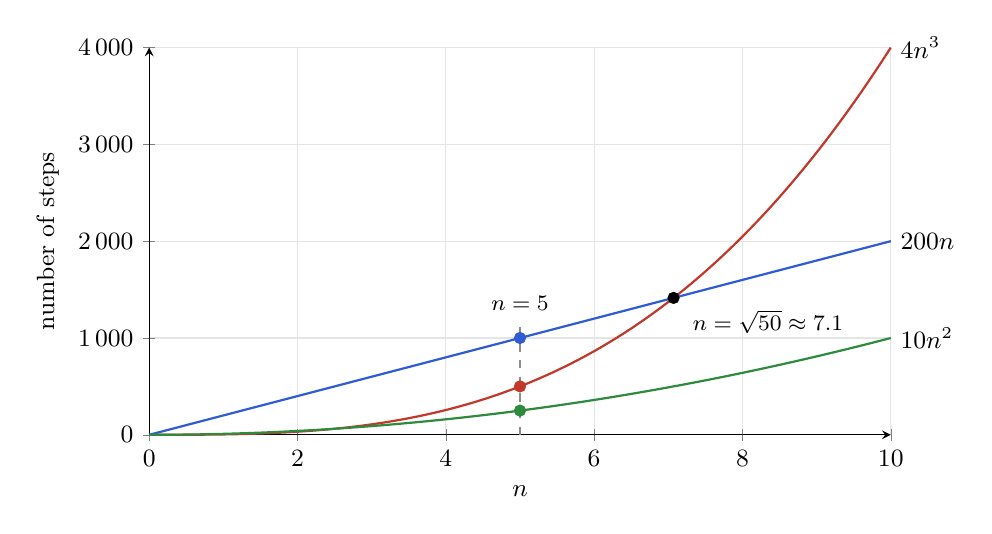
\begin{tikzpicture}
\begin{axis}[
  width=11cm,height=6.5cm,
  xmin=0,xmax=10,ymin=0,ymax=4000,
  xtick={0,2,...,10},ytick={0,1000,...,4000},
  scaled y ticks=false,
  yticklabel style={/pgf/number format/1000 sep={\,}},
  xlabel={$n$},ylabel={number of steps},
  axis lines=left,grid=major,grid style={black!10},
  label style={font=\small},tick label style={font=\small},
  domain=0:10,samples=101,clip=false]
  \addplot[thick,PlotRed] {4*x^3};
  \addplot[thick,PlotBlue] {200*x};
  \addplot[thick,PlotGreen] {10*x^2};
  \node[right,font=\small] at (axis cs:10,4000) {$4n^3$};
  \node[right,font=\small] at (axis cs:10,2000) {$200n$};
  \node[right,font=\small] at (axis cs:10,1000) {$10n^2$};
  \draw[dashed,black!45] (axis cs:5,0) -- (axis cs:5,1180);
  \node[above,font=\footnotesize] at (axis cs:5,1180) {$n=5$};
  \addplot[only marks,mark=*,mark size=2pt,PlotRed] coordinates {(5,500)};
  \addplot[only marks,mark=*,mark size=2pt,PlotBlue] coordinates {(5,1000)};
  \addplot[only marks,mark=*,mark size=2pt,PlotGreen] coordinates {(5,250)};
  \addplot[only marks,mark=*,mark size=2pt,black] coordinates {(7.0711,1414.2)};
  \node[anchor=north west,font=\footnotesize]
    at (axis cs:7.2,1390) {$n=\sqrt{50}\approx7.1$};
\end{axis}
\end{tikzpicture}
\end{center}

For small $n$, a lower-order term can be the largest. At $n=5$ we
have
\[
  200n=1000,\qquad 4n^3=500,\qquad 10n^2=250.
\]
As $n$ grows, however, the cubic term overtakes $200n$ at
$n=\sqrt{50}\approx7.1$ and dominates from then on, so it determines
the running time.

\textbf{Upper bound.} For $n\geq1$, every power of $n$ in $T(n)$ is at
most $n^3$, so
\[
  T(n)\leq 4n^3+10n^3+200n^3+7n^3=221\,n^3.
\]
Hence $T(n)=O(n^3)$, with $c=221$ and $n_0=1$.

\textbf{Lower bound.} All the terms are non-negative, so
\[
  T(n)\geq 4n^3.
\]
Hence $T(n)=\Omega(n^3)$, with $c=4$ and $n_0=1$.

\textbf{Conclusion.} Therefore, by
Proposition~\ref{prop:theta-from-bounds}, $T(n)=\Theta(n^3)$.

\textbf{Other upper bounds.} For $n\geq1$,
\[
  T(n)\leq221\,n^3\leq221\,n^4\leq221\,n^5,
\]
so we also have $T(n)=O(n^4)$ and $T(n)=O(n^5)$. However,
$T(n)\neq\Theta(n^4)$: since $T(n)/n^4\leq221/n\to0$, no constant
$c>0$ gives $T(n)\geq c\,n^4$ for all large $n$.
\end{framedexample}

When analysing an algorithm we are mostly interested in the
\emph{upper bound}, that is, in the worst case. Often we do not know
exactly how many times a step runs. In
Algorithm~\ref{alg:max-find}, we do not know in advance how many
times the update $\mathit{max}\gets A[i]$ will run, but in the worst
case (a sorted array) it runs $n$ times, so it never runs more than $n$
times. Bounding each step from above gives an upper bound on $T(n)$.

\subsection{Comparing growth rates}

\begin{framedprop}{Growth rates}\label{prop:growth-rates}
For large $n$ (that is, up to constants and eventually):
\begin{itemize}
  \item $n^c\leq n^d$ for $c\leq d$;
  \item $\log^c n=(\log n)^c\leq n^d$ for all constants $c,d>0$;
  \item $n^c\leq d^n$ for every constant $c$ and every $d>1$;
  \item more generally, $n^c\leq d^{an^b}$ for $d>1$ and constants
    $a,b>0$.
\end{itemize}
Consequently,
\begin{align*}
  1&\leq\log\log n\leq\log n\leq\log^2 n\leq\sqrt n\leq n\\
   &\leq n\log\log n\leq n\log n\leq n\sqrt n\leq n^2\leq n^3\leq 2^n.
\end{align*}
\end{framedprop}

For example, $(\log n)^{10}$ and $\sqrt n$: the logarithm raised to
any power always loses eventually, so $\sqrt n$ grows faster.

\begin{notebox}[The base of the logarithm does not matter]
Changing the base of a logarithm only multiplies it by a constant:
\[
  \log_2 n=\frac{\log_{10}n}{\log_{10}2}
          =\underbrace{\frac{1}{\log_{10}2}}_{\text{constant}}
           \cdot\log_{10}n.
\]
Asymptotically all bases are equivalent, so we simply write
$O(\log n)$.
\end{notebox}

An exponential running time means that the algorithm is extremely slow:
an algorithm with exponential running time is hopeless except for tiny
inputs. Ideally we would like logarithmic or linear running times.

\begin{center}
\begin{tabular}{rcccc}
  \toprule
  $n$ & $\log_2 n$ & $n\log_2 n$ & $n^2$ & $2^n$\\
  \midrule
  $10$   & $3.3$  & $33$    & $10^2$ & $\approx1.0\cdot10^{3}$\\
  $100$  & $6.6$  & $664$   & $10^4$ & $\approx1.3\cdot10^{30}$\\
  $1000$ & $10.0$ & $9966$  & $10^6$ & $\approx1.1\cdot10^{301}$\\
  \bottomrule
\end{tabular}
\end{center}

\section{Lower bounds and optimal algorithms}

Max-Find is correct and runs in time $\Theta(n)$. Could we do better,
say $O(\sqrt n)$? No: any correct algorithm must read every element,
because an element it never reads could be the maximum. With $n$
elements to read, no algorithm can beat $\Omega(n)$.

\begin{frameddefn}{Lower bound and optimal algorithm}
\label{def:optimal-algorithm}
A problem has \emph{lower bound} $\Omega(g(n))$ if every algorithm
that solves it needs $\Omega(g(n))$ steps in the worst case. An
algorithm is (asymptotically) \emph{optimal} if its running time
matches a lower bound for the problem.
\end{frameddefn}

\begin{framedexample}{Max-Find is optimal}\label{ex:max-find-optimal}
Max-Find (Algorithm~\ref{alg:max-find}) runs in $O(n)$, as we computed
in Example~\ref{ex:max-find-steps}, and the problem requires
$\Omega(n)$, so Max-Find is \emph{optimal}.
\end{framedexample}

\section{Prefix sums}

\begin{framedproblem}{Prefix sums}\label{prob:prefix-sums}
\textbf{Input:} an array $A$ of length $n$.\\
\textbf{Output:} an array $S$ of length $n$ such that, for every $i$,
\[
  S[i]=\sum_{j=1}^{i}A[j].
\]
\end{framedproblem}

For example, $A=[3,6,-2,-5,8]$ gives $S=[3,9,7,2,10]$.

\subsection{A quadratic algorithm}

The direct approach computes each sum from scratch.

\Needspace{14\baselineskip}
\begin{framedalgo}{Prefix sums, direct version}\label{alg:prefix-slow}
\begin{algorithmic}[1]
  \State $n\gets\mathrm{length}(A)$ \Comment{$1$ step}
  \For{$i=1$ \textbf{to} $n$} \Comment{$n$ steps}
    \State $S[i]\gets0$ \Comment{$n$ steps}
    \For{$j=1$ \textbf{to} $i$} \Comment{$i$ times for the $i$-th element}
      \State $S[i]\gets S[i]+A[j]$ \Comment{$i$ times}
    \EndFor
  \EndFor
  \State \Return $S$ \Comment{$1$ step}
\end{algorithmic}
\end{framedalgo}

The inner loop runs once for the first element, twice for the second,
and $n$ times for the last. Each of its two lines therefore runs
\[
  1+2+3+\cdots+n=\sum_{i=1}^{n}i=\frac{n(n+1)}{2}
\]
times, and
\[
  T(n)=1+n+n+2\cdot\frac{n(n+1)}{2}+1=n^2+3n+2=\Theta(n^2).
\]

\begin{notebox}[A quicker upper bound]
We do not need the exact sum. For every $i$, the inner loop runs at
most $n$ times, so
\[
  T(n)\leq 2n+n\cdot(2n)+2=O(n^2).
\]
Bounding each loop by its largest possible number of iterations is
often enough to obtain an upper bound.
\end{notebox}

\subsection{Closing the gap}

Is this algorithm optimal? No: the lower bound for the problem is
$\Omega(n)$ (we must read every element), while our algorithm takes
$\Theta(n^2)$. There is a \emph{gap}, and we can try to close it by
finding a better algorithm. The key observation is that each prefix
sum extends the previous one:
\[
  S[i]=\sum_{j=1}^{i}A[j]=\sum_{j=1}^{i-1}A[j]+A[i]=S[i-1]+A[i].
\]

\Needspace{10\baselineskip}
\begin{framedalgo}{Prefix sums, fast version}\label{alg:prefix-fast}
\begin{algorithmic}[1]
  \State $n\gets\mathrm{length}(A)$
  \State $S[1]\gets A[1]$
  \For{$i=2$ \textbf{to} $n$}
    \State $S[i]\gets S[i-1]+A[i]$ \Comment{$n-1$ times}
  \EndFor
  \State \Return $S$
\end{algorithmic}
\end{framedalgo}

Now $T(n)=\Theta(n)$, which matches the lower bound: the fast version
is optimal.

\section{An open gap: matrix multiplication}

Let $A,B\in\R^{n\times n}$ and $C=AB$. Each entry is
\[
  C[i,j]=\sum_{k=1}^{n}A[i,k]\,B[k,j].
\]
Computing one entry takes $n$ multiplications, and there are $n^2$
entries, so the direct algorithm runs in $\Theta(n^3)$.

A lower bound is $\Omega(n^2)$: the output matrix $C$ has $n^2$ values,
and we must compute each of them. For many years, researchers have
tried to close the gap between $n^2$ and $n^3$. The gap has been
reduced, but it has not yet been closed.

\begin{notebox}[For reference]
Strassen's algorithm (1969) multiplies two $n\times n$ matrices in
$O(n^{\log_2 7})\approx O(n^{2.81})$ operations. The best known
exponent today is about $2.37$, still above the lower bound $2$.
\end{notebox}

\chapter{Recursion}

\section{Fibonacci numbers}

\begin{frameddefn}{Fibonacci sequence}\label{def:fibonacci}
\[
  \mathrm{fib}(n)=
  \begin{cases}
    1, & n=0\text{ or }n=1,\\
    \mathrm{fib}(n-1)+\mathrm{fib}(n-2), & n\geq2.
  \end{cases}
\]
\end{frameddefn}

\begin{center}
\begin{tabular}{c|cccccccccc}
  $n$ & 0 & 1 & 2 & 3 & 4 & 5 & 6 & 7 & 8 & 9\\
  \hline
  $\mathrm{fib}(n)$ & 1 & 1 & 2 & 3 & 5 & 8 & 13 & 21 & 34 & 55
\end{tabular}
\end{center}

The definition is \emph{recursive}: it defines $\mathrm{fib}(n)$ in
terms of smaller values. It translates directly into a recursive
algorithm, one that calls itself.

\Needspace{12\baselineskip}
\begin{framedalgo}{Recursive Fibonacci}\label{alg:fib-recursive}
\begin{algorithmic}[1]
  \Function{Fibonacci}{$n$}
    \If{$n=0$ \textbf{or} $n=1$} \Comment{$1$ step}
      \State \Return $1$ \Comment{at most $1$ step}
    \EndIf
    \State $f_1\gets$ \Call{Fibonacci}{$n-1$} \Comment{$T(n-1)$ steps}
    \State $f_2\gets$ \Call{Fibonacci}{$n-2$} \Comment{$T(n-2)$ steps}
    \State \Return $f_1+f_2$ \Comment{$1$ step}
  \EndFunction
\end{algorithmic}
\end{framedalgo}

\subsection{Running time of the recursive algorithm}

Let $T(n)$ be the number of steps for input $n$. Counting the steps of
Algorithm~\ref{alg:fib-recursive} gives a \emph{recurrence}:
\[
  T(n)=
  \begin{cases}
    2, & n=0\text{ or }n=1,\\
    T(n-1)+T(n-2)+3, & n\geq2.
  \end{cases}
\]
The formula is recursive. How can we solve it? A first idea is to
expand it. The recurrence holds for \emph{every} $n\geq2$, so we can
apply it to the terms on the right as well: replacing $n$ with $n-1$
gives $T(n-1)=T(n-2)+T(n-3)+3$, and replacing $n$ with $n-2$ gives
$T(n-2)=T(n-3)+T(n-4)+3$. In the computations below, each underlined
term is replaced, in the next line, by the expression underlined in the
same colour.

\textbf{First expansion.}
\begin{align*}
  T(n)&=\cul{PlotRed}{T(n-1)}+\cul{PlotBlue}{T(n-2)}+3\\
      &=\cul{PlotRed}{\bigl[T(n-2)+T(n-3)+3\bigr]}
        +\cul{PlotBlue}{\bigl[T(n-3)+T(n-4)+3\bigr]}+3\\
      &=T(n-2)+2T(n-3)+T(n-4)+9.
\end{align*}

\textbf{Second expansion.} We expand each of the three terms again:
\begin{align*}
  T(n)&=\cul{PlotRed}{T(n-2)}+\cul{PlotBlue}{2T(n-3)}
        +\cul{PlotGreen}{T(n-4)}+9\\
      &=\cul{PlotRed}{\bigl[T(n-3)+T(n-4)+3\bigr]}
        +\cul{PlotBlue}{2\bigl[T(n-4)+T(n-5)+3\bigr]}\\
      &\qquad+\cul{PlotGreen}{\bigl[T(n-5)+T(n-6)+3\bigr]}+9\\
      &=T(n-3)+3T(n-4)+3T(n-5)+T(n-6)+21=\cdots
\end{align*}
The expansion stops when the arguments reach $0$ or $1$. After two
expansions the smallest argument is already $n-6$, and the number of
terms keeps growing: we may suspect that $T(n)$ is exponential.

\begin{framedprop}{The recursive algorithm is exponential}
\label{prop:fib-exponential}
The running time of Algorithm~\ref{alg:fib-recursive} satisfies
\[
  T(n)=\Omega\bigl(2^{n/2}\bigr)=\Omega\bigl((\sqrt2)^n\bigr).
\]
\end{framedprop}

\begin{proof}
$T$ is non-decreasing: $T(1)=T(0)$, and for $n\geq2$ we have
$T(n)\geq T(n-1)$. \Needspace{14\baselineskip}
Replacing $T(n-1)$ with the smaller $T(n-2)$,
\[
  T(n)=T(n-1)+T(n-2)+3\geq 2\,\cul{PlotRed}{T(n-2)}+3.
\]
Applying the same inequality repeatedly,
\begin{align*}
  T(n)&\geq 2\,\cul{PlotRed}{\bigl(2T(n-4)+3\bigr)}+3
        =4\,\cul{PlotBlue}{T(n-4)}+9\\
      &\geq 4\,\cul{PlotBlue}{\bigl(2T(n-6)+3\bigr)}+9
        =8\,\cul{PlotGreen}{T(n-6)}+21\\
      &\geq 8\,\cul{PlotGreen}{\bigl(2T(n-8)+3\bigr)}+21=16T(n-8)+45\\
      &\;\;\vdots\\
      &\geq 2^iT(n-2i)+3(2^i-1)\geq 2^iT(n-2i)
      \qquad\text{after $i$ steps.}
\end{align*}
For even $n$, take $i=n/2$:
\[
  T(n)\geq 2^{n/2}\,T(0)=2\cdot2^{n/2}=2(\sqrt2)^n.
\]
For odd $n$, take $i=(n-1)/2$ and use $T(1)=2$ in the same way.
\end{proof}

Why is it so slow? To compute $\mathrm{fib}(n)$, the algorithm makes
two calls, $\mathrm{fib}(n-1)$ and $\mathrm{fib}(n-2)$, each of which
makes two more calls, and so on. It computes the same values a lot of
times, again and again: the work roughly doubles at each level of the
recursion tree.

\begin{center}
\begin{tikzpicture}[
  level distance=1.25cm,
  level 1/.style={sibling distance=6.2cm},
  level 2/.style={sibling distance=3.1cm},
  level 3/.style={sibling distance=1.55cm},
  every node/.style={font=\small,inner sep=2pt},
  r2/.style={fill=NotesExample!55,rounded corners=2pt},
  r3/.style={fill=NotesProposition!55,rounded corners=2pt}]
  \node {$f(n)$}
    child {node {$f(n-1)$}
      child {node[r2] {$f(n-2)$}
        child {node[r3,font=\footnotesize] {$f(n-3)$}}
        child {node[font=\footnotesize] {$f(n-4)$}}}
      child {node[r3] {$f(n-3)$}
        child {node[font=\footnotesize] {$f(n-4)$}}
        child {node[font=\footnotesize] {$f(n-5)$}}}}
    child {node[r2] {$f(n-2)$}
      child {node[r3] {$f(n-3)$}
        child {node[font=\footnotesize] {$f(n-4)$}}
        child {node[font=\footnotesize] {$f(n-5)$}}}
      child {node {$f(n-4)$}
        child {node[font=\footnotesize] {$f(n-5)$}}
        child {node[font=\footnotesize] {$f(n-6)$}}}};
\end{tikzpicture}

{\small Here $f(k)$ stands for a call to $\mathrm{fib}(k)$. Already in
the first levels, $f(n-2)$ is computed twice and $f(n-3)$ three times.}
\end{center}

\subsection{Avoiding repeated work}

There are two ways to fix the problem:
\begin{itemize}
  \item \textbf{Store the values} (memoization): using some memory, we
    compute each $\mathrm{fib}(k)$ once and look it up afterwards.
  \item \textbf{Compute bottom-up}: start from the base cases and fill
    the table from left to right, $1+1=2$, $2+1=3$, $3+2=5$,
    $5+3=8$, \ldots, each value being the sum of the previous two.
\end{itemize}

\Needspace{14\baselineskip}
\begin{framedalgo}{Iterative Fibonacci}\label{alg:fib-iterative}
\begin{algorithmic}[1]
  \Function{FibonacciIterative}{$n$}
    \If{$n\leq1$}
      \State \Return $1$
    \EndIf
    \State $\mathit{previous}\gets1$ \Comment{$\mathrm{fib}(0)$}
    \State $\mathit{current}\gets1$ \Comment{$\mathrm{fib}(1)$}
    \For{$i=2$ \textbf{to} $n$}
      \State $\mathit{new}\gets\mathit{previous}+\mathit{current}$
      \State $\mathit{previous}\gets\mathit{current}$
      \State $\mathit{current}\gets\mathit{new}$
    \EndFor
    \State \Return $\mathit{current}$
  \EndFunction
\end{algorithmic}
\end{framedalgo}

The loop runs $n-1$ times with a constant amount of work per iteration,
so the running time is $T(n)=O(n)$: this algorithm is linear.

\begin{notebox}[Indexing and closed form]
The slides use the convention $F_0=0$, $F_1=1$ (their iterative
algorithm returns $n$ for $n\leq1$ and starts from $0$ and $1$). With
that convention $\mathrm{fib}(n)=F_{n+1}$, so the two sequences differ
only by a shift. There is also a closed formula, which we do not prove:
\[
  F_n=\frac{1}{\sqrt5}\left[\left(\frac{1+\sqrt5}{2}\right)^{n}
     -\left(\frac{1-\sqrt5}{2}\right)^{n}\right],
  \qquad
  \mathrm{fib}(n)=F_{n+1}.
\]
\end{notebox}

\lecturestart{1 October}

\section{Binary search}

\begin{framedproblem}{Search}\label{prob:search}
\textbf{Input:} an array $A$ of $n$ numbers and a value $x$.\\
\textbf{Output:} \textsc{true} if $x$ is in $A$, \textsc{false}
otherwise.
\end{framedproblem}

We could compare $x$ with every element, with linear complexity.
If $A$ is \emph{sorted}, we do not need to check all the elements: we
look at the central element and compare it with $x$. If $x$ is larger,
it can only be in the right half; if smaller, only in the left half.
We then repeat on that half.

\begin{framedexample}{Searching a sorted array}\label{ex:binary-search}
Let $A=[1,3,7,10,13,24,30,33,39,55]$ and $x=39$.
\begin{enumerate}
  \item The central element is $A[5]=13<39$, so we keep the right part
    $[24,30,33,39,55]$.
  \item Its central element is $33<39$, so we keep $[39,55]$.
  \item Its central element is $39=x$: found.
\end{enumerate}
\end{framedexample}

\Needspace{16\baselineskip}
\begin{framedalgo}{Binary search}\label{alg:binary-search}
\begin{algorithmic}[1]
  \Function{BinarySearch}{$A,x$}
    \State $n\gets\mathrm{len}(A)$
    \If{$n=0$}
      \State \Return \textsc{false}
    \EndIf
    \If{$x<A[1]$ \textbf{or} $x>A[n]$} \Comment{$x$ outside the range of $A$}
      \State \Return \textsc{false}
    \EndIf
    \State $\mathit{mid}\gets\lceil n/2\rceil$
    \If{$x=A[\mathit{mid}]$}
      \State \Return \textsc{true}
    \ElsIf{$x<A[\mathit{mid}]$}
      \State \Return \Call{BinarySearch}{$A[1,\ldots,\mathit{mid}-1],x$}
    \Else
      \State \Return \Call{BinarySearch}{$A[\mathit{mid}+1,\ldots,n],x$}
    \EndIf
  \EndFunction
\end{algorithmic}
\end{framedalgo}

The \emph{ceiling} $\lceil y\rceil$ is the smallest integer greater
than or equal to $y$: for example, $\lceil3\rceil=3$ and
$\lceil3.1\rceil=4$.

\begin{framedexample}{An unsuccessful search}\label{ex:binary-search-fail}
Let $A=[13,17]$ and $x=15$.
\begin{enumerate}
  \item Since $13<15<17$, $x$ lies within the range of $A$.
  \item The central element is $A[1]=13<15$ (here
    $\mathit{mid}=\lceil2/2\rceil=1$), so we keep the right part $[17]$.
  \item Now $15<17$, so $x$ is outside the range of $[17]$: the
    algorithm returns \textsc{false}.
\end{enumerate}
\end{framedexample}

\subsection{Running time}

Every line of Algorithm~\ref{alg:binary-search} takes constant time,
except the recursive call. The call works on an array of half the size,
so it takes $T(n/2)$ steps instead of $T(n)$:
\[
  T(n)=
  \begin{cases}
    c_1, & n\leq1,\\
    T(n/2)+c_2, & \text{otherwise},
  \end{cases}
\]
where $c_1$ and $c_2$ are constants. For $n\geq2$,
\begin{align*}
  T(n)&=T\!\left(\tfrac n2\right)+c_2
       =T\!\left(\tfrac n4\right)+2c_2
       =T\!\left(\tfrac n8\right)+3c_2
       =\cdots
       =T\!\left(\tfrac{n}{2^i}\right)+i\,c_2.
\end{align*}
We stop when the array has size $1$, that is, when $n/2^i=1$, or
$i=\log_2 n$. Then $T(n/2^i)=T(1)=c_1$ and
\[
  T(n)=c_1+c_2\log_2 n=\Theta(\log n).
\]

\begin{notebox}[Subarrays]
We treat $A[1,\ldots,\mathit{mid}-1]$ as a view of the original array,
described by its first and last index. Copying the subarray at every
call would cost linear time and destroy the logarithmic bound.
\end{notebox}

We cannot do better than $\Theta(\log n)$, but we are not able to prove
this yet. Splitting into three parts instead of two does not help
asymptotically: the recurrence becomes $T(n)=T(n/3)+c_2'$, so
$T(n)=O(\log_3 n)$, and $O(\log_3 n)=O(\log_2 n)$ because
$\log_3 n=\log_2 n/\log_2 3$.

\chapter{Complexity classes}

\section{The traveling salesman problem}

We want to visit all the nodes of a weighted graph, starting from a
node and coming back to it, while minimizing the total cost. Every
order of visit gives a tour, and different tours have different costs.

\begin{framedproblem}{Traveling salesman problem (TSP)}\label{prob:tsp}
\textbf{Input:} $n$ cities and the cost of travelling between each pair
of them.\\
\textbf{Output:} a tour that visits every city exactly once and returns
to the starting city, with minimum total cost.
\end{framedproblem}

\begin{framedexample}{Four cities}\label{ex:tsp-four}
\begin{center}
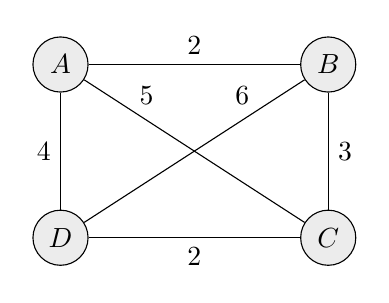
\begin{tikzpicture}[city/.style={circle,draw,fill=gray!15,
    minimum size=7mm,inner sep=0pt}]
  \node[city] (A) at (0,2.2) {$A$};
  \node[city] (B) at (3.4,2.2) {$B$};
  \node[city] (C) at (3.4,0) {$C$};
  \node[city] (D) at (0,0) {$D$};
  \draw (A) -- node[above] {2} (B);
  \draw (B) -- node[right] {3} (C);
  \draw (C) -- node[below] {2} (D);
  \draw (D) -- node[left] {4} (A);
  \draw (A) -- node[pos=0.22,above right=-1pt] {5} (C);
  \draw (B) -- node[pos=0.22,above left=-1pt] {6} (D);
\end{tikzpicture}
\end{center}
Starting from $A$, there are $3!=6$ orders of visit, which give three
distinct tours (each one can be travelled in two directions):
\begin{align*}
  A\,B\,C\,D\,A&:\ 2+3+2+4=11,\\
  A\,B\,D\,C\,A&:\ 2+6+2+5=15,\\
  A\,C\,B\,D\,A&:\ 5+3+6+4=18.
\end{align*}
The optimal tour costs $11$. In the lecture graph with eight cities,
two tours cost $15$ and $21$.
\end{framedexample}

The brute-force approach tries all tours:
with $n$ cities there are $(n-1)!$ orders of visit, and
\[
  n!=1\cdot2\cdot3\cdots(n-1)\cdot n\geq1\cdot2\cdot2\cdots2=2^{n-1},
\]
so the factorial grows even faster than an exponential: this is not
good at all. No known algorithm finds the shortest tour quickly.

\section{Decision problems, P and NP}

We usually study \emph{decision problems}, whose answer is yes or no.
An optimization problem such as minimizing costs or maximizing profits
becomes a decision problem by fixing a threshold. For TSP: \emph{is
there a tour that visits all the nodes with total cost at most $14$?}
If the answer is yes, we can ask whether we can do better, for example
cost at most $13$.

\begin{frameddefn}{The class P}\label{def:class-p}
$\mathrm{P}$ is the class of problems that we can solve in
\emph{polynomial time} (poly-time), that is, in time $O(n^k)$ for some
constant $k$.
\end{frameddefn}

\begin{frameddefn}{The class NP}\label{def:class-np}
$\mathrm{NP}$ is the class of problems for which, if someone gives us
a candidate solution, we can verify in polynomial time whether the
answer is \textsc{yes}.
\end{frameddefn}

\begin{framedexample}{Easy to verify}\label{ex:np-verify}
\begin{itemize}
  \item \emph{Rubik's cube}: it is easy to check whether a cube is
    solved.
  \item \emph{TSP}: given a tour, we add up its costs and check whether
    the total is at most $14$.
  \item \emph{Sudoku}: it is easy to check whether a filled grid is
    correct.
\end{itemize}
What these problems have in common is that, given a solution, we can
verify in poly-time whether it is correct, even though finding one may
be hard.
\end{framedexample}

Max-Find and binary search are in $\mathrm{P}$. Every problem in
$\mathrm{P}$ is also in $\mathrm{NP}$: if we can solve a problem
quickly, we can verify an answer by solving it ourselves. Hence
$\mathrm{P}\subseteq\mathrm{NP}$.

\begin{notebox}[What NP stands for]
NP stands for \emph{nondeterministic polynomial time}, not ``non
polynomial''. A problem in NP may well be easy: every problem in P is
in NP.
\end{notebox}

Are there problems in NP that are not in P? Nobody knows.
\begin{center}
\emph{Is $\mathrm{P}=\mathrm{NP}$, or is $\mathrm{P}\subsetneq\mathrm{NP}$?
We don't know.}
\end{center}
This is one of the most important open questions in computer science.

\begin{center}
\begin{tikzpicture}
  \draw[fill=gray!12] (0,0) ellipse (3.6cm and 2.0cm);
  \node at (-1.7,1.35) {NP};
  \draw[fill=NotesProposition!45] (1.35,-0.1) circle (1.3cm);
  \node at (1.35,0.8) {P};
  \node[font=\footnotesize,align=center] at (1.35,-0.2) {Max-Find\\binary search};
  \draw[fill=NotesTheorem!45] (-1.45,-0.15) circle (1.05cm);
  \node[font=\footnotesize,align=center] at (-1.45,-0.15) {TSP\\SAT\\Knapsack};
  \node[font=\small] (npc) at (-3.7,-1.9) {NP-complete};
  \draw[->] (npc) -- (-1.9,-1.05);
  \node[font=\small] at (0,-2.45) {if $\mathrm{P}\neq\mathrm{NP}$};
  \begin{scope}[xshift=7cm]
    \draw[fill=NotesProposition!45] (0,0) circle (1.6cm);
    \node at (0,0) {$\mathrm{P}=\mathrm{NP}$};
    \node[font=\small] at (0,-2.45) {if $\mathrm{P}=\mathrm{NP}$};
  \end{scope}
\end{tikzpicture}
\end{center}

\section{Reductions and NP-completeness}

Some problems in NP are as hard as any other problem in NP.

\begin{frameddefn}{NP-complete problem}\label{def:np-complete}
A problem $X$ is \emph{NP-complete} if:
\begin{enumerate}
  \item $X\in\mathrm{NP}$;
  \item every problem $Y\in\mathrm{NP}$ can be \emph{reduced} in
    polynomial time to $X$.
\end{enumerate}
\end{frameddefn}

A reduction of $Y$ to $X$ solves $Y$ using an algorithm for $X$ plus a
polynomial amount of extra work.

\begin{framedexample}{Max-Find and sorting}\label{ex:reduction-sort-max}
If we can sort an array in poly-time, we can also find its maximum in
poly-time: sort it and take the last element. Max-Find reduces to
sorting.

The converse also holds: if we can find the maximum, we put it in the
last position and repeat on the remaining elements, until the whole
array is sorted. This uses $n$ calls to Max-Find, a polynomial amount
of work, so sorting reduces to Max-Find.
\end{framedexample}

Surprisingly, NP-complete problems exist, such as \emph{SAT} (Boolean
satisfiability), which we will not study in detail. If
$\mathrm{P}=\mathrm{NP}$, the classes collapse: NP-complete problems
would be solvable in polynomial time, like every other problem in NP.

\begin{notebox}[Are TSP, Sudoku and Rubik's cube NP-complete?]
Complexity classes describe how the cost grows with the input size, so
we must consider generalized versions of these puzzles:
\begin{itemize}
  \item the decision version of TSP (``is there a tour of cost at most
    $k$?'') is NP-complete;
  \item Sudoku on $n^2\times n^2$ grids (``can this partially filled
    grid be completed?'') is NP-complete;
  \item for the $n\times n\times n$ Rubik's cube, deciding whether a
    position can be solved in at most $k$ moves is NP-complete
    (proved in 2018).
\end{itemize}
The classic $9\times9$ Sudoku and $3\times3\times3$ cube have a fixed
size, so asymptotic statements do not apply to them directly.
\end{notebox}

\lecturestart{5 October}

\begin{framedcor}{Solving one NP-complete problem}\label{cor:np-complete}
Let $X$ be NP-complete. If $X$ can be solved in poly-time, then every
problem in $\mathrm{NP}$ can be solved in poly-time. Equivalently, if
some $Y\in\mathrm{NP}$ cannot be solved in poly-time, then neither can
$X$.
\end{framedcor}

SAT was the first problem proved to be NP-complete: every problem in
$\mathrm{NP}$ can be reduced to SAT (the Cook--Levin theorem). To show
that a new problem is NP-complete, we no longer need to reduce every
problem in NP to it.

\begin{framedprop}{Proving NP-completeness}\label{prop:prove-npc}
To prove that a problem $X$ is NP-complete, show that:
\begin{enumerate}
  \item $X\in\mathrm{NP}$;
  \item there is a problem $Y$ already known to be NP-complete and a
    poly-time reduction of $Y$ to $X$.
\end{enumerate}
\end{framedprop}

This works because reductions compose: every problem in NP reduces to
$Y$, and $Y$ reduces to $X$, so every problem in NP reduces to $X$.
The composition of two polynomials is still a polynomial.

\begin{center}
\begin{tikzpicture}[>=Stealth,
  box/.style={draw,rounded corners,inner sep=5pt,fill=NotesTheorem!35}]
  \node (y1) at (-3.2,0.9) {$Y_1$};
  \node (y2) at (-3.2,0.1) {$Y_2$};
  \node (y3) at (-3.2,-0.75) {$\vdots$};
  \node[box] (sat) at (0,0) {SAT};
  \node[box] (x) at (3.4,0) {$X$};
  \node (z) at (6.2,0) {$Z$};
  \draw[->] (y1) -- (sat);
  \draw[->] (y2) -- (sat);
  \draw[->] (y3) -- (sat);
  \draw[->,thick] (sat) -- node[above,font=\small] {poly-time} (x);
  \draw[->,thick] (x) -- node[above,font=\small] {poly-time} (z);
  \node[font=\small,align=center] at (-3.2,-1.6) {every problem\\in NP};
\end{tikzpicture}
\end{center}

\section{Some NP-complete problems}

\subsection{Knapsack}

We want to fill a backpack with the most valuable set of items without
exceeding its capacity.

\begin{framedproblem}{Knapsack}\label{prob:knapsack}
\textbf{Input:} a set of items $I=\{1,2,\ldots,n\}$, where item $i$
has a weight $w_i$ and a value $v_i$, and a budget $B$.\\
\textbf{Output:} a subset of items $S\subseteq I$ such that
\[
  \sum_{i\in S}w_i\leq B
  \qquad\text{that maximizes}\qquad
  \sum_{i\in S}v_i.
\]
\end{framedproblem}

\begin{framedexample}{A knapsack instance}\label{ex:knapsack}
Let $B=55$ and
\begin{center}
\begin{tabular}{c|ccccccc}
  $i$   & 1  & 2  & 3 & 4  & 5  & 6  & 7\\
  \hline
  $w_i$ & 10 & 20 & 6 & 30 & 15 & 20 & 50\\
  $v_i$ & 10 & 15 & 8 & 17 & 12 & 17 & 20
\end{tabular}
\end{center}
We must maximize $\sum_{i\in S}v_i$ subject to the constraint
$\sum_{i\in S}w_i\leq55$. One feasible solution is $S=\{1,2,3,5\}$,
with total weight $51$ and total value $45$. A solution taken ``at
random'' like this one is probably not the best: in
Example~\ref{ex:greedy-knapsack} we will find one of value $47$.
\end{framedexample}

\subsection{Set cover}

Suppose we want to rob a casino: we need people who can do different
things.

\begin{framedproblem}{Set cover}\label{prob:set-cover}
\textbf{Input:} a task that requires the skills $s_1,\ldots,s_n$, and
$m$ experts $E_1,\ldots,E_m$, where each $E_i\subseteq\{1,\ldots,n\}$
is the subset of skills that expert $i$ has.\\
\textbf{Output:} the smallest number of experts that together cover
all the skills.
\end{framedproblem}

In general, the skills are elements $e_1,\ldots,e_n$ and the experts
are sets $S_1,\ldots,S_m$ of elements. We want the minimum number of
sets whose union contains all the elements.

\begin{framedexample}{Covering six skills}\label{ex:set-cover}
\begin{center}
\begin{tabular}{c|cccccc}
      & $s_1$ & $s_2$ & $s_3$ & $s_4$ & $s_5$ & $s_6$\\
  \hline
  $E_1$ & $\times$ &  & $\times$ & $\times$ &  & \\
  $E_2$ & $\times$ & $\times$ &  &  &  & \\
  $E_3$ &  & $\times$ &  &  & $\times$ & \\
  $E_4$ & $\times$ &  &  & $\times$ &  & $\times$\\
  $E_5$ &  &  & $\times$ &  &  & $\times$
\end{tabular}
\end{center}
We must take $E_3$, because it is the only expert with skill $s_5$.
$E_3$ covers $s_2$ and $s_5$; no single other expert covers all of
$s_1,s_3,s_4,s_6$, so we need at least $3$ experts. One optimal
solution is $\{E_3,E_4,E_5\}$.
\end{framedexample}

A heuristic method: take $E_3$, then repeatedly take the expert who
covers the largest number of skills not yet covered. Such solutions
are not optimal in general.

\subsection{Subset sum}

\begin{framedproblem}{Subset sum}\label{prob:subset-sum}
\textbf{Input:} a list of integers.\\
\textbf{Output:} a nonempty sublist whose elements sum to $0$, if one
exists.
\end{framedproblem}

For the list $[3,7,-3,-8,10,-16,2,9]$, the sublists $[3,-3]$ and
$[7,9,-16]$ both sum to $0$.

\subsection{Maximum clique}

\begin{framedproblem}{Maximum clique}\label{prob:max-clique}
\textbf{Input:} a graph.\\
\textbf{Output:} a largest \emph{clique}, that is, a largest set of
nodes that are all connected to one another.
\end{framedproblem}

\begin{center}
\begin{tikzpicture}[v/.style={circle,draw,fill=gray!15,minimum size=5mm,
    inner sep=0pt},
  k/.style={very thick,NotesTheorem!80!black}]
  \node[v] (a) at (0,0) {};
  \node[v] (b) at (2,0) {};
  \node[v] (c) at (2,1.8) {};
  \node[v] (d) at (0,1.8) {};
  \node[v] (e) at (3.8,0.9) {};
  \node[v] (f) at (-1.8,0.9) {};
  \node[v] (g) at (3.8,2.4) {};
  \draw[k] (a)--(b) (b)--(c) (c)--(d) (d)--(a) (a)--(c) (b)--(d);
  \draw (b)--(e) (c)--(e) (e)--(g) (c)--(g) (f)--(a) (f)--(d);
\end{tikzpicture}

{\small The thick edges form a clique of size $4$, the largest in this
graph.}
\end{center}

\Needspace{9\baselineskip}
\begin{framedprop}{Some NP-complete problems}\label{prop:npc-examples}
The decision versions of Knapsack, Set cover, Subset sum and Max clique
are NP-complete.
\end{framedprop}

We do not prove this: each proof is a poly-time reduction from a known
NP-complete problem (Proposition~\ref{prop:prove-npc}).

\section{NP-hard problems}

\begin{frameddefn}{NP-hard problem}\label{def:np-hard}
A problem $X$ is \emph{NP-hard} if every problem in $\mathrm{NP}$ can
be reduced to $X$ in polynomial time. Unlike an NP-complete problem,
$X$ does not have to belong to $\mathrm{NP}$.
\end{frameddefn}

NP-hard problems are more general: NP-complete means NP-hard and in
NP. For example, the optimization versions of Knapsack and TSP (find
the best solution, not just answer yes or no) are NP-hard.

\begin{notebox}[Minimum spanning tree]
The minimum spanning tree problem is \emph{not} NP-hard (unless
$\mathrm{P}=\mathrm{NP}$): Kruskal's and Prim's algorithms solve it in
polynomial time. Its relative, the Steiner tree problem, which must
connect only a given subset of the nodes, is NP-hard.
\end{notebox}

\chapter{Approximation and heuristics}

For NP-complete and NP-hard problems we do not know fast exact
algorithms. Two ways out are approximation algorithms, which come with
a guarantee, and heuristics, which do not.

\section{Approximation algorithms}

\begin{frameddefn}{$c$-approximation algorithm}\label{def:approximation}
Let $c\geq1$. For an input $I$, let $\OPT_I$ be the value of an optimal
solution. A \emph{$c$-approximation algorithm} returns, for every input
$I$, a solution whose value is
\begin{itemize}
  \item at most $c\cdot\OPT_I$, for a \emph{minimization} problem;
  \item at least $\OPT_I/c$, for a \emph{maximization} problem.
\end{itemize}
\end{frameddefn}

\begin{framedexample}{Reading the guarantee}\label{ex:approximation}
\begin{itemize}
  \item \emph{TSP (minimization)}: suppose that for an input $I$ the
    optimal tour costs $\OPT_I=5000$. A $2$-approximation algorithm
    guarantees a tour of cost at most $10\,000$: it may cost more than
    $5000$, but we are sure that it does not exceed $10\,000$. For
    $c=1.1$, the tour costs at most $1.1\cdot5000=5500$, no more than
    $10\%$ above the optimum.
  \item \emph{Knapsack (maximization)}: if $\OPT_I=1000$, a
    $1.1$-approximation guarantees a value of at least
    $1000/1.1\approx909$.
\end{itemize}
\end{framedexample}

\subsection{Guarantees without knowing the optimum}

How can we prove that a solution is a $c$-approximation if we cannot
find the optimal solution? We may not find $\OPT_I$, but we can often
find a \emph{lower bound} $L\leq\OPT_I$ (for a minimization problem).
Then
\[
  \frac{\text{output}}{\OPT_I}\leq\frac{\text{output}}{L}.
\]

\begin{framedexample}{Using a lower bound}\label{ex:lower-bound-ratio}
\begin{center}
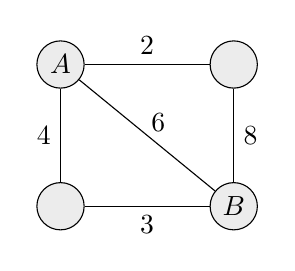
\begin{tikzpicture}[v/.style={circle,draw,fill=gray!15,minimum size=6mm,
    inner sep=0pt}]
  \node[v] (A) at (0,1.8) {$A$};
  \node[v] (T) at (2.2,1.8) {};
  \node[v] (B) at (2.2,0) {$B$};
  \node[v] (L) at (0,0) {};
  \draw (A) -- node[above] {2} (T);
  \draw (T) -- node[right] {8} (B);
  \draw (A) -- node[above right=-2pt] {6} (B);
  \draw (A) -- node[left] {4} (L);
  \draw (L) -- node[below] {3} (B);
\end{tikzpicture}
\end{center}
Suppose every solution must travel from $A$ to $B$. Every route from
$A$ to $B$ costs at least $6$, so $\OPT_I\geq6$: $6$ is a lower bound.
If our algorithm outputs a solution of cost $17$, is it good?
\[
  \frac{\text{output}}{\OPT_I}=\frac{17}{\OPT_I}\leq\frac{17}{6}
  \approx2.83,
\]
so our solution is at most $17/6$ times the optimum.
\end{framedexample}

\lecturestart{8 October}

\subsection{How well can we approximate?}

Different problems behave very differently:
\begin{itemize}
  \item For \emph{set cover}, where we minimize the number of sets, a
    simple greedy algorithm is, at worst, an $O(\log n)$-approximation.
  \item Many other problems cannot be approximated well in poly-time.
    For \emph{max clique}, no polynomial-time algorithm can guarantee
    even a factor like $\sqrt n$, unless $\mathrm{P}=\mathrm{NP}$.
\end{itemize}
Some approximation algorithms are also very inefficient. This is why
there is another approach: heuristics.

\section{Heuristics}

A \emph{heuristic} is a method that usually finds good solutions
quickly, but without any guarantee on their quality.

\subsection{A greedy heuristic for knapsack}

For each item, consider the value per unit of weight
\[
  r_i=\frac{v_i}{w_i}.
\]
We start putting into the backpack the items with the largest $r_i$,
and keep adding items as long as the constraint is satisfied. This
usually gives a good solution, but not always the optimal one.

\Needspace{12\baselineskip}
\begin{framedalgo}{Greedy knapsack}\label{alg:greedy-knapsack}
\begin{algorithmic}[1]
  \State sort the items so that $r_{i_1}\geq r_{i_2}\geq\cdots\geq r_{i_n}$
  \State $S\gets\varnothing$, $W\gets0$
  \For{$k=1$ \textbf{to} $n$}
    \If{$W+w_{i_k}\leq B$}
      \State $S\gets S\cup\{i_k\}$, $W\gets W+w_{i_k}$
    \EndIf
  \EndFor
  \State \Return $S$
\end{algorithmic}
\end{framedalgo}

\begin{framedexample}{Greedy on the knapsack instance}
\label{ex:greedy-knapsack}
For the instance in Example~\ref{ex:knapsack},
\[
  r_1=1,\quad r_2=\tfrac34,\quad r_3=\tfrac43,\quad r_4=\tfrac{17}{30},
  \quad r_5=\tfrac45,\quad r_6=\tfrac{17}{20},\quad r_7=\tfrac25.
\]
Item $3$ has the largest ratio, so it is the first one we add. The
order is $3,1,6,5,2,4,7$:
\begin{itemize}
  \item add $3$ (weight $6$), $1$ (weight $16$), $6$ (weight $36$) and
    $5$ (weight $51$);
  \item items $2$, $4$ and $7$ no longer fit ($51+20>55$).
\end{itemize}
The result is $S=\{1,3,5,6\}$, with weight $51$ and value $47$. Trying
all subsets shows that $47$ is optimal for this instance.
\end{framedexample}

The greedy solution is not optimal in general.

\begin{framedexample}{When greedy fails}\label{ex:greedy-fails}
Let $B=100$, ten items with $w_1=\cdots=w_{10}=50$ and
$v_1=\cdots=v_{10}=50$ (each with ratio $1$), and an item $0$ with
$w_0=51$ and $v_0=52$, whose ratio is slightly larger than $1$.
Greedy takes item $0$ first, and then no other item fits
($51+50>100$): the value is $52$. Taking two items of weight $50$
gives value $100$.
\end{framedexample}

No known algorithm solves knapsack in poly-time: it is NP-complete. If
we could ``break'' the items and take a fraction of one of them (the
\emph{fractional} knapsack), the greedy algorithm would be perfect: we
fill the remaining capacity with a fraction of the next item.

\subsection{Greedy algorithms and meta-heuristics}

\begin{frameddefn}{Greedy algorithm}\label{def:greedy}
A \emph{greedy} algorithm makes, at each step, the choice that is best
for now, hoping that it will also work well in the future, and
continues in the same way.
\end{frameddefn}

The knapsack heuristic above and the set cover heuristic are both
greedy algorithms. Greediness is an example of a \emph{meta-heuristic}:
a general strategy, a wider class that includes many heuristics.
Another example is \emph{local search}: starting from a solution, such
as a tour, we try small modifications (for example, exchanging two of
its edges for two others) and keep those that improve it, searching
for the optimal one.

\chapter{Distance measures}

\section{Why distances?}

Many problems ask us to find distances or similarities between
objects. For example, given some documents and a query, we want the
documents most similar to the query; or we want groups of similar
documents, a \emph{cluster}. The input is a set of objects and the
output a group of them. To do this we use different kinds of
distances: a function that measures the distance between two elements
defines a relation between them.

\section{Distance functions}

\begin{frameddefn}{Distance function}\label{def:distance}
Let $U$ be a universe of elements (documents, objects, strings, \ldots).
A \emph{distance function} is a map
\[
  d:U\times U\longrightarrow\R,
\]
taking two elements and returning a number, which satisfies, for all
$x,y,z\in U$:
\begin{enumerate}
  \item $d(x,y)\geq0$, and $d(x,y)=0$ if and only if $x=y$;
  \item $d(x,y)=d(y,x)$ (symmetry);
  \item $d(x,y)\leq d(x,z)+d(z,y)$ (triangle inequality).
\end{enumerate}
\end{frameddefn}

\begin{center}
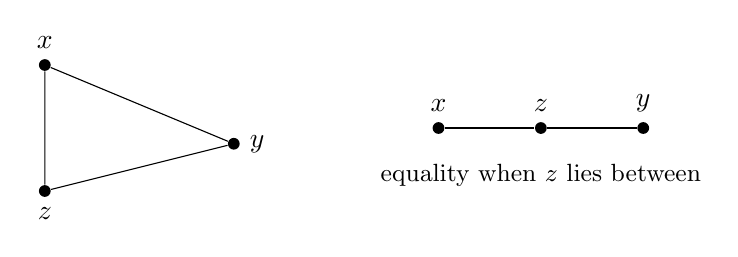
\begin{tikzpicture}[p/.style={circle,fill=black,inner sep=1.5pt}]
  \node[p,label=above:$x$] (x) at (0,1.6) {};
  \node[p,label=right:$y$] (y) at (2.4,0.6) {};
  \node[p,label=below:$z$] (z) at (0,0) {};
  \draw (x) -- (y) (x) -- (z) (z) -- (y);
  \begin{scope}[xshift=5cm,yshift=0.8cm]
    \node[p,label=above:$x$] (x2) at (0,0) {};
    \node[p,label=above:$z$] (z2) at (1.3,0) {};
    \node[p,label=above:$y$] (y2) at (2.6,0) {};
    \draw (x2) -- (z2) -- (y2);
    \node[font=\small] at (1.3,-0.6) {equality when $z$ lies between};
  \end{scope}
\end{tikzpicture}
\end{center}

We should define distances that make sense for the problem: what does
it mean for two objects to be ``close''? It depends on the problem we
are considering.

\section{\texorpdfstring{$L_p$}{Lp} distances}

We have defined what a distance function is
(Definition~\ref{def:distance}). We now look at concrete distances,
starting with objects described by vectors of numbers, that is,
$U=\R^m$.

Suppose we are designing an app like Google Maps that shows the
restaurants near us. On the map, our position and each restaurant are
points with two coordinates, that is, vectors in $\R^2$. To decide
which restaurants are near, we need a distance between two points. The
natural choice is the length of the straight segment that joins them:
the Euclidean distance. The same formula works for vectors with any
number $m$ of coordinates.

\begin{frameddefn}{Euclidean distance}\label{def:euclidean}
For $U=\R^m$, $\vec x=[x_1,\ldots,x_m]$ and $\vec y=[y_1,\ldots,y_m]$,
the \emph{Euclidean distance}, or $L_2$ distance, is
\[
  d(\vec x,\vec y)=\sqrt{\sum_{j=1}^{m}(x_j-y_j)^2}.
\]
\end{frameddefn}

It is clearly non-negative and symmetric; it also satisfies the
triangle inequality, but we do not prove it.

\begin{frameddefn}{$L_p$ distance}\label{def:lp-distance}
For a constant $p\geq1$,
\[
  d_p(\vec x,\vec y)
  =\left(\sum_{j=1}^{m}\abs{x_j-y_j}^p\right)^{1/p}
  =\norm{\vec x-\vec y}_p.
\]
\end{frameddefn}

Changing $p$ gives different distances, which weigh the differences
between coordinates differently:
\begin{itemize}
  \item $p=2$: the Euclidean distance.
  \item $p=1$: the \emph{Manhattan distance},
    $\sum_j\abs{x_j-y_j}$.
  \item $p\to\infty$: the $L_\infty$ distance,
    $\displaystyle d_\infty(\vec x,\vec y)
      =\max_{i\in\{1,\ldots,m\}}\abs{x_i-y_i}$.
  \item ``$L_0$'': the number of coordinates in which the vectors
    differ, $\abs{\{i:x_i\neq y_i\}}$. For binary strings this is the
    \emph{Hamming distance}.
\end{itemize}

\begin{framedexample}{Counting the coordinates that differ}
\label{ex:hamming}
\begin{itemize}
  \item The binary strings $00110$ and $10100$ differ in $2$ positions
    (the first and the fourth), so their Hamming distance is $2$.
  \item The vectors $[3,1,3]$ and $[0,1,3]$ differ only in the first
    coordinate, so their $L_0$ distance is $1$.
\end{itemize}
\end{framedexample}

\begin{framedexample}{Comparing $L_p$ distances}\label{ex:lp-distances}
Let
\[
  \vec x=[3,7,0,2,1],\qquad
  \vec y=[4,5,10,7,3],\qquad
  \vec z=[5,2,5,6,5].
\]
The coordinate differences are $\abs{\vec x-\vec y}=[1,2,10,5,2]$ and
$\abs{\vec x-\vec z}=[2,5,5,4,4]$.
\begin{center}
\begin{tabular}{ccc}
  \toprule
  $p$ & $\norm{\vec x-\vec y}_p$ & $\norm{\vec x-\vec z}_p$\\
  \midrule
  $1$ & $1+2+10+5+2=20$ & $2+5+5+4+4=20$\\
  $2$ & $(1+4+100+25+4)^{1/2}\approx11.58$
      & $(4+25+25+16+16)^{1/2}\approx9.27$\\
  $3$ & $(1+8+1000+125+8)^{1/3}\approx10.45$
      & $(8+125+125+64+64)^{1/3}\approx7.28$\\
  $\infty$ & $10$ & $5$\\
  \bottomrule
\end{tabular}
\end{center}
With $p=1$ the two distances are equal. As $p$ increases, both
distances decrease, and the larger differences weigh more: $\vec y$
differs from $\vec x$ by $10$ in one coordinate, so it ends up farther
than $\vec z$, whose differences are moderate everywhere.
\end{framedexample}

\section{Distances between sets}

So far we have worked with vectors. Now imagine that we want to
compare the customers of a supermarket based on what they bought.

\begin{framedexample}{Shopping baskets}\label{ex:baskets}
Each letter is a product: the first person bought apples ($A$),
bananas ($B$), carrots ($C$) and donuts ($D$):
\[
  P_1=\{A,B,C,D\},\qquad
  P_2=\{A,E,G,H\},\qquad
  P_3=\{B,C,E,F\}.
\]
Intuitively, persons $1$ and $3$ are more similar than persons $1$
and $2$.
\end{framedexample}

\subsection{Sets as binary vectors}

We can write each set as a binary vector, with one coordinate per
product, and use the $L_1$ distance:
\begin{center}
\begin{tabular}{c|cccccccc}
      & $A$ & $B$ & $C$ & $D$ & $E$ & $F$ & $G$ & $H$\\
  \hline
  $P_1$ & 1 & 1 & 1 & 1 & 0 & 0 & 0 & 0\\
  $P_2$ & 1 & 0 & 0 & 0 & 1 & 0 & 1 & 1\\
  $P_3$ & 0 & 1 & 1 & 0 & 1 & 1 & 0 & 0
\end{tabular}
\end{center}
Then $\abs{P_1-P_2}=[0,1,1,1,1,0,1,1]$ and
$\abs{P_1-P_3}=[1,0,0,1,1,1,0,0]$, so
\[
  \norm{P_1-P_2}_1=6,\qquad\norm{P_1-P_3}_1=4.
\]
So $P_1$ is closer to $P_3$, as we expected. In general,
\[
  \norm{P-Q}_1=\abs{P}+\abs{Q}-2\abs{P\cap Q}=\abs{P\mathbin{\triangle}Q},
\]
the size of the \emph{symmetric difference} $P\mathbin{\triangle}Q$,
the elements in exactly one of the two sets.

\subsection{Counting common items}

The formula above depends on the intersection $P\cap Q$. Let us look
at the elements in common directly:
\[
  \abs{P_1\cap P_2}=1,\qquad\abs{P_1\cap P_3}=2.
\]
Is this a good distance? We should check the three properties.
Symmetry certainly holds, but the larger the value, the \emph{closer}
the two sets: this is a \emph{similarity}, not a distance. It is often
more natural to talk about similarity than about distance.

\begin{frameddefn}{Similarity function}\label{def:similarity}
A \emph{similarity function} is a map $s:U\times U\to\R$ such that
$s(x,y)=s(y,x)$ for all $x,y\in U$, and whose value is larger the more
similar $x$ and $y$ are. Similarities are often normalized to take
values in $[0,1]$, with $s(x,x)=1$ for every $x$.
\end{frameddefn}

Unlike distances, similarities have no standard list of properties:
the ones above are the usual conventions. The two notions go in
opposite directions: a large similarity means a small distance. Here
we do not see a ``natural'' distance function, and we cannot simply
take the negative of the similarity, because distances cannot be
negative.

\subsection{Normalizing the intersection}

The size of the intersection alone, however, is misleading. Two pairs
of sets can have intersections of the same size, but if the sets in the
second pair are smaller, the intersection is a larger fraction of them,
so they are more similar.

\begin{center}
\begin{tikzpicture}
  \begin{scope}
    \clip (0,0) circle (1.1);
    \fill[NotesExample!60] (1.7,0) circle (1.1);
  \end{scope}
  \draw (0,0) circle (1.1) (1.7,0) circle (1.1);
  \node at (0.85,-1.5) {\small $1$};
  \begin{scope}[xshift=5.2cm]
    \begin{scope}
      \clip (0,0) circle (0.65);
      \fill[NotesExample!60] (0.7,0) circle (0.65);
    \end{scope}
    \draw (0,0) circle (0.65) (0.7,0) circle (0.65);
    \node at (0.35,-1.5) {\small $2$};
  \end{scope}
\end{tikzpicture}

{\small Same intersection, different set sizes: the sets in pair $2$
are more similar, because their intersection is a larger fraction of
them.}
\end{center}

We can normalize the intersection in several ways:
\[
  \frac{\abs{P\cap Q}}{\max\{\abs P,\abs Q\}},\qquad
  \frac{\abs{P\cap Q}}{\abs{P\cup Q}},\qquad
  \frac{\abs{P\cap Q}}{\abs P+\abs Q}.
\]

\begin{frameddefn}{Jaccard similarity}\label{def:jaccard}
The \emph{Jaccard similarity} of two finite sets $P$ and $Q$ is
\[
  J(P,Q)=\frac{\abs{P\cap Q}}{\abs{P\cup Q}},
\]
where $\abs{\cdot}$ is the cardinality (not the absolute value).
\end{frameddefn}

The Jaccard similarity is symmetric, lies between $0$ and $1$, and
gives $J(P,P)=1$ for every nonempty $P$: it is a normalized similarity
function (Definition~\ref{def:similarity}). For the baskets in
Example~\ref{ex:baskets},
\[
  J(P_1,P_2)=\frac{\abs{\{A\}}}{\abs{\{A,B,C,D,E,G,H\}}}=\frac17,
  \qquad
  J(P_1,P_3)=\frac{\abs{\{B,C\}}}{\abs{\{A,B,C,D,E,F\}}}=\frac26=\frac13,
\]
so $P_1$ is more similar to $P_3$, as expected.

\begin{frameddefn}{Jaccard distance}\label{def:jaccard-distance}
We turn the Jaccard similarity into a distance by taking
\[
  d_J(P,Q)=1-\frac{\abs{P\cap Q}}{\abs{P\cup Q}}
          =\frac{\abs{P\cup Q}-\abs{P\cap Q}}{\abs{P\cup Q}}
          =\frac{\abs{P\mathbin{\triangle}Q}}{\abs{P\cup Q}}
          =\frac{\abs{P\setminus Q}+\abs{Q\setminus P}}{\abs{P\cup Q}}.
\]
\end{frameddefn}

\begin{center}
\begin{tikzpicture}
  \fill[NotesExample!60,even odd rule] (0,0) circle (1) (1.3,0) circle (1);
  \draw (0,0) circle (1) (1.3,0) circle (1);
  \node at (-0.4,0) {$P$};
  \node at (1.7,0) {$Q$};
\end{tikzpicture}

{\small The symmetric difference $P\mathbin{\triangle}Q$: everything
except the intersection.}
\end{center}

One can prove that the Jaccard distance $d_J$ is a distance in the
sense of Definition~\ref{def:distance}. For the baskets,
$d_J(P_1,P_2)=6/7$ and $d_J(P_1,P_3)=4/6=2/3$.

\chapter{Distances between strings}

\lecturestart{12 October}

\section{Why compare strings?}

Biological data are sequences of bases such as
\texttt{CTAGGATCGGAC}, and DNA sequences have particular properties: we
may want to know how ``similar'' two parts of DNA are. Search engines
need similarity between strings too: if we type ``Sceince'' instead
of ``Science'' on Google, it still understands what we mean.

\begin{framedexample}{Which strings are closer?}\label{ex:three-strings}
\[
  X=\texttt{CTAGGAT},\qquad
  Y=\texttt{CCAGAGT},\qquad
  Z=\texttt{AGCCCTA}.
\]
Which pair is more similar, $X$ and $Y$, or $X$ and $Z$? We would say
$X$ and $Y$. The answer is intuitive, but which property are we using?
How do we define a ``distance measure'' between strings?
\end{framedexample}

\section{First attempts}

\begin{itemize}
  \item \textbf{Compare letter by letter.} We could compare the strings
    position by position, as with the Hamming or $L_1$ distance. But
    what if the strings have different lengths?
  \item \textbf{Letters as numbers.} Another idea that might come to
    mind is to associate each letter with its position in the alphabet
    ($A=1$, $C=3$, $G=7$, $T=20$) and to compute the $L_1$ distance
    between the resulting vectors. For example,
    \[
      \begin{array}{r@{\quad}cccc}
        \texttt{CAGT}: & 3 & 1 & 7 & 20\\
        \texttt{ACTT}: & 1 & 3 & 20 & 20\\
        \hline
        \text{difference}: & 2 & 2 & 13 & 0
      \end{array}
      \qquad\Longrightarrow\qquad 2+2+13+0=17.
    \]
    The larger the number, the farther the strings, and the distance
    is symmetric. However, it does not work well:
    \begin{itemize}
      \item \texttt{SAPIENZA} and \texttt{SSAPIENZA}, typed with an
        extra \texttt{S} by mistake, are almost identical, but the
        extra letter shifts all the following ones and the distance
        explodes;
      \item the distance between $A$ and $T$ is larger than between
        $A$ and $B$ only because of the alphabetical order.
    \end{itemize}
  \item \textbf{Count the characters.} We could count how many times
    each character appears. Biologically, however, \texttt{AAGGGTT}
    and \texttt{TGAAGTG} are very different, even though they contain
    exactly the same characters.
  \item \textbf{Look at common pieces.} \texttt{CATGAGG} and
    \texttt{CAGAGT} share \texttt{CA} and \texttt{GAG}, even though
    they have different lengths.
  \item \textbf{Count modifications.} We could take the second string
    and count how many changes are needed to make it equal to the
    first. For \texttt{SAPIENZA} and \texttt{SAAPIEMZA}, we delete the
    extra \texttt{A} and replace \texttt{M} with \texttt{N}: two
    changes, so the distance is $2$.
\end{itemize}

The last two ideas are the promising ones: common pieces lead to
subsequences, and modifications lead to the edit distance. Consider
sequences over an alphabet.

\section{Subsequences}

\begin{frameddefn}{Subsequence}\label{def:subsequence}
A \emph{subsequence} of a sequence $S$ is a sequence that contains a
subset of the characters of $S$ in the same order, not necessarily
consecutive.
\end{frameddefn}

\begin{framedexample}{Subsequences}\label{ex:subsequences}
For $S=\texttt{ATCGGACTGA}$, all of the following are subsequences:
\texttt{ATCGGACTGA} itself, \texttt{ACGGCTA}, \texttt{AAA}, and the
empty string.
\end{framedexample}

\begin{frameddefn}{Common subsequence}\label{def:common-subsequence}
Given two sequences $S$ and $T$, a \emph{common subsequence} is a
sequence that is a subsequence of both $S$ and $T$.
\end{frameddefn}

For $S=\texttt{ATGCATG}$ and $T=\texttt{AGACTAG}$, \texttt{AAT} and
\texttt{AGAG} are common subsequences, and so is the empty string.

\subsection{The longest common subsequence}

\begin{frameddefn}{Longest common subsequence (LCS)}\label{def:lcs}
The \emph{longest common subsequence} of $S$ and $T$ is a common
subsequence of maximum length. We write $\LCS(S,T)$ for its length.
\end{frameddefn}

We can define the similarity of two strings as the length of their
LCS.

\begin{framedexample}{Longest common subsequences}\label{ex:lcs}
\begin{itemize}
  \item For \texttt{ATGA} and \texttt{TAG}, both \texttt{AG} and
    \texttt{TG} are longest common subsequences: the LCS need not be
    unique, and here none is longer than $2$.
  \item Compare \texttt{SAPEMZA} with \texttt{SAPIENZA} and with
    \texttt{SALERNO}:
    \[
      \LCS(\texttt{SAPIENZA},\texttt{SAPEMZA})=6\ (\texttt{SAPEZA}),
      \qquad
      \LCS(\texttt{SAPEMZA},\texttt{SALERNO})=3\ (\texttt{SAE}).
    \]
    \texttt{SAPEMZA} has more in common with \texttt{SAPIENZA} than
    with \texttt{SALERNO}.
  \item In Example~\ref{ex:three-strings},
    $\LCS(X,Y)=5$ (for example \texttt{CAGGT}) while $\LCS(X,Z)=3$
    (\texttt{CTA}), which confirms our intuition.
  \item For \texttt{CAGTGACCGATAC} and \texttt{GACCAGTCAGCAC} it is
    already hard to find the LCS by hand. Its length is $8$, for
    example \texttt{CAGTGCAC}.
\end{itemize}
\end{framedexample}

Checking all subsequences is not an option: a string of length $k$ has
up to $2^k$ subsequences, one for each subset of its positions, so
brute force needs about $2^{\min\{\abs S,\abs T\}}$ checks.

\section{Edit distance}

How do we compare two strings? Option 1: transform one string into the
other. Option 2: look at their subsequences. The two options turn out
to be closely related.

\begin{frameddefn}{Edit distance}\label{def:edit-distance}
Given two sequences $S$ and $T$, the \emph{edit distance} $\ED(S,T)$
is the minimum number of insertions and deletions of characters needed
to transform $S$ into $T$.
\end{frameddefn}

\begin{framedexample}{Transforming a string}\label{ex:edit-distance}
Let $S=\texttt{CATGA}$ and $T=\texttt{ACTGC}$:
\[
  \texttt{CATGA}
  \xrightarrow{\text{delete }\texttt{C}}\texttt{ATGA}
  \xrightarrow{\text{insert }\texttt{C}}\texttt{ACTGA}
  \xrightarrow{\text{insert }\texttt{C}}\texttt{ACTGAC}
  \xrightarrow{\text{delete }\texttt{A}}\texttt{ACTGC}.
\]
Four changes suffice, and in fact $\ED(S,T)=4$.
\end{framedexample}

We could also delete all the letters one by one and insert the new
ones, but that is not the shortest way. When the strings are longer,
it is hard to see the minimum number of steps.

The edit distance is symmetric, $\ED(S,T)=\ED(T,S)$, because we can
perform all the steps in reverse: each insertion becomes a deletion
and vice versa.

\begin{notebox}[Substitutions]
Some definitions also allow \emph{substitutions}, replacing one
character with another at cost $1$. With insertions and deletions
only, a substitution costs $2$: one deletion and one insertion.
\end{notebox}

\subsection{Edit distance and LCS}

A natural strategy for transforming $S$ into $T$: find an LCS, delete
everything else from $S$, leaving only the LCS, and then insert the
characters of $T$ that are missing.

\begin{framedprop}{Edit distance from the LCS}\label{prop:ed-lcs}
\[
  \ED(S,T)
  =\underbrace{\bigl(\abs S-\LCS(S,T)\bigr)}_{\text{characters to delete}}
  +\underbrace{\bigl(\abs T-\LCS(S,T)\bigr)}_{\text{characters to insert}}
  =\abs S+\abs T-2\LCS(S,T).
\]
\end{framedprop}

\begin{proof}[Why it holds]
The strategy above uses exactly $\abs S+\abs T-2\LCS(S,T)$ operations,
so $\ED(S,T)$ is at most this number. Conversely, in any sequence of
insertions and deletions, the characters of $S$ that are never deleted
appear in $T$ in the same order: they form a common subsequence, of
some length $k\leq\LCS(S,T)$. We must then delete at least $\abs S-k$
characters and insert at least $\abs T-k$, so at least
$\abs S+\abs T-2k\geq\abs S+\abs T-2\LCS(S,T)$ operations are needed.
\end{proof}

For Example~\ref{ex:edit-distance}, $\LCS(\texttt{CATGA},\texttt{ACTGC})=3$
(for example \texttt{CTG}), so $\ED=5+5-2\cdot3=4$.

\section{A recursive formula for the edit distance}

The optimal algorithm for computing the edit distance is not obvious.
We now write a recursive formula, the starting point of
\emph{dynamic programming}.

\begin{notebox}[Notation]
Consider two strings $S$ and $T$ with $\abs S=n$ and $\abs T=m$:
\[
  S=[S[1],S[2],\ldots,S[n]],\qquad T=[T[1],\ldots,T[m]].
\]
We write $S^i=[S[1],\ldots,S[i]]$ and $T^j=[T[1],\ldots,T[j]]$ for the
\emph{prefixes} of length $i$ and $j$.
\end{notebox}

\begin{framedprop}{Recurrence for the edit distance}\label{prop:ed-recurrence}
\[
  \ED(S^i,T^j)=
  \begin{cases}
    j, & \text{if } i=0,\\
    i, & \text{if } j=0,\\
    \ED(S^{i-1},T^{j-1}), & \text{if } S[i]=T[j],\\
    \min\bigl\{\ED(S^i,T^{j-1}),\,\ED(S^{i-1},T^j)\bigr\}+1,
      & \text{if } S[i]\neq T[j].
  \end{cases}
\]
\end{framedprop}

\begin{itemize}
  \item If one string is empty, we must insert (or delete) all the
    characters of the other.
  \item If the last characters are equal, we do not need to modify
    them: we can ignore them and consider the distance between
    $S^{i-1}$ and $T^{j-1}$. For example,
    \[
      \ED(\texttt{CATGCAT\,T},\texttt{ACCTAGAC\,T})
      =\ED(\texttt{CATGCAT},\texttt{ACCTAGAC}).
    \]
  \item If the last characters differ, one of them must go: either we
    remove the last character of $S$, giving $\ED(S^{i-1},T^j)+1$, or
    we remove the last character of $T$ (equivalently, we insert it at
    the end of $S$), giving $\ED(S^i,T^{j-1})+1$. For
    \texttt{CATGCAT\,T} and \texttt{ACCTAGAC\,A}, we remove either the
    \texttt{T} or the \texttt{A}. We take the better of the two
    options.
\end{itemize}

\begin{framedexample}{Small edit distances}\label{ex:small-ed}
\begin{itemize}
  \item $\ED(\texttt{TGA},\texttt{TTA})=2$: we must remove
    \texttt{G} and add \texttt{T}. Also $\ED(\texttt{TG},\texttt{TT})=2$,
    because we have to remove a character and then add one.
  \item For \texttt{CAG} and \texttt{TGA}, the last characters
    differ. Either we remove \texttt{G} from \texttt{CAG}, which leaves
    \texttt{CA} and \texttt{TGA} ($+1$); or we remove \texttt{A} from
    \texttt{TGA}, which leaves \texttt{CAG} and \texttt{TG} ($+1$),
    whose last characters are now equal. Both options lead to
    $\ED(\texttt{CAG},\texttt{TGA})=4$.
\end{itemize}
\end{framedexample}

\Needspace{14\baselineskip}
\begin{framedalgo}{Recursive edit distance}\label{alg:ed-recursive}
\begin{algorithmic}[1]
  \Function{ED}{$S^i,T^j$}
    \If{$i=0$}
      \State \Return $j$
    \ElsIf{$j=0$}
      \State \Return $i$
    \ElsIf{$S[i]=T[j]$}
      \State \Return \Call{ED}{$S^{i-1},T^{j-1}$}
    \Else
      \State \Return $1+\min\bigl\{$\Call{ED}{$S^i,T^{j-1}$},
        \Call{ED}{$S^{i-1},T^j$}$\bigr\}$
    \EndIf
  \EndFunction
\end{algorithmic}
\end{framedalgo}

Written directly as a recursive algorithm, this formula has an
exponential running time.

\begin{notebox}[The same problem as Fibonacci]
As with the recursive Fibonacci algorithm
(Proposition~\ref{prop:fib-exponential}), the recursion solves the
same subproblems again and again. There are only $(n+1)(m+1)$
different subproblems $\ED(S^i,T^j)$, so storing each value once
(dynamic programming) avoids the repeated work.
\end{notebox}

\chapter{Memory and data representation}\label{ch:memory-representation}

\lecturestart{19 October}

\section{Bytes, addresses and consecutive memory locations}

\textbf{What is memory for?}
While a program runs, it needs somewhere to keep the data it is
working with: numbers, text, lists and the intermediate results of
calculations. Main memory (RAM) provides this working space, so the
processor can read the data, perform operations and store the results
for later steps of the program.

For example, after executing \texttt{x = 5}, Python must keep the
object representing $5$ available. A later instruction such as
\texttt{print(x)} can retrieve it, and \texttt{x + 2} can use it to
compute $7$. Understanding how data are arranged and reached in
memory will help us explain the cost of operations such as accessing
an element of a list.

\begin{frameddefn}{Bit and byte}\label{def:bit-byte}
A \emph{bit} is a binary digit, either $0$ or $1$.
A \emph{byte} consists of eight bits.
\end{frameddefn}

Imagine memory as numbered cells, drawn vertically below. Each cell
holds one byte. The number on the left is its address: it identifies
the cell, while the contents are stored inside it.
\begin{center}
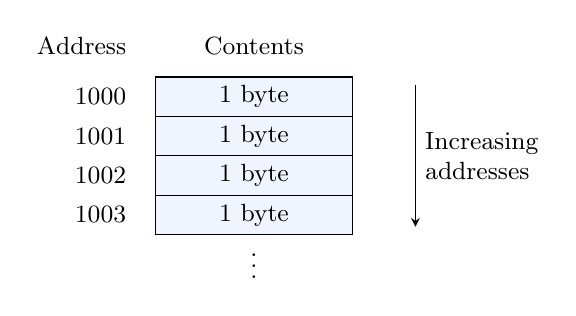
\begin{tikzpicture}[font=\small,>=stealth]
  \node[anchor=east] at (-0.25,0.4) {Address};
  \node at (1.25,0.4) {Contents};
  \foreach \i in {0,...,3} {
    \pgfmathtruncatemacro{\address}{1000+\i}
    \draw[fill=PlotBlue!7] (0,-0.5*\i) rectangle (2.5,-0.5*\i-0.5);
    \node[anchor=east] at (-0.25,-0.5*\i-0.25) {$\address$};
    \node at (1.25,-0.5*\i-0.25) {1 byte};
  }
  \node at (1.25,-2.3) {$\vdots$};
  \draw[->] (3.3,-0.1) -- (3.3,-1.9)
    node[midway,right,align=left] {Increasing\\addresses};
\end{tikzpicture}
\end{center}
The address and the contents are different things: the label $1000$
tells us where the first displayed byte is, not what value it holds.
We use illustrative decimal addresses throughout these drawings.

\begin{frameddefn}{Memory address}\label{def:memory-address}
In byte-addressable memory, a \emph{memory address} identifies the
location of one byte. The address specifies \emph{where} data are
stored; the contents are the data stored at that location.
\end{frameddefn}

\begin{framedexample}{A block occupying eight consecutive bytes}
Suppose a piece of data occupies eight bytes starting at address
$1000$. Follow the addresses down the drawing:
\begin{center}
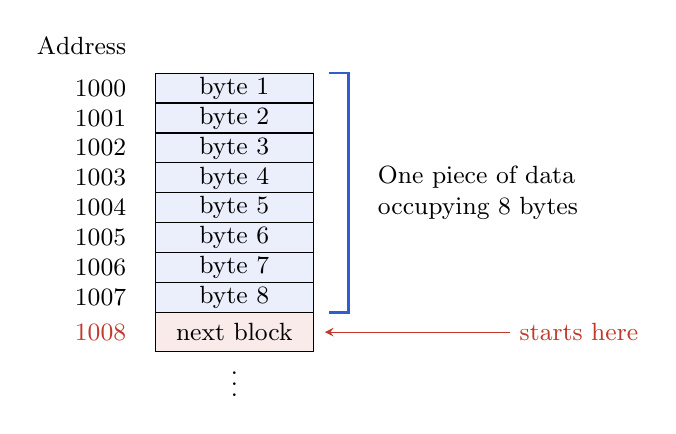
\begin{tikzpicture}[font=\small,>=stealth]
  \node[anchor=east] at (-0.25,0.35) {Address};
  \foreach \i in {0,...,7} {
    \pgfmathtruncatemacro{\address}{1000+\i}
    \pgfmathtruncatemacro{\byteindex}{\i+1}
    \draw[fill=PlotBlue!10] (0,-0.38*\i) rectangle (2,-0.38*\i-0.38);
    \node[anchor=east] at (-0.25,-0.38*\i-0.19) {$\address$};
    \node at (1,-0.38*\i-0.19) {byte \byteindex};
  }
  \draw[thick,PlotBlue] (2.2,0) -- (2.45,0) -- (2.45,-3.04) -- (2.2,-3.04);
  \node[anchor=west,align=left] at (2.7,-1.52) {One piece of data\\occupying 8 bytes};
  \draw[fill=PlotRed!10] (0,-3.04) rectangle (2,-3.54);
  \node[anchor=east,text=PlotRed] at (-0.25,-3.29) {$1008$};
  \node at (1,-3.29) {next block};
  \draw[->,PlotRed] (4.5,-3.29) -- (2.15,-3.29);
  \node[anchor=west,text=PlotRed] at (4.5,-3.29) {starts here};
  \node at (1,-3.85) {$\vdots$};
\end{tikzpicture}
\end{center}
The starting byte is already the first of the eight, so the last
byte is at $1000+7=1007$. The first address \emph{after} the block is
\[
  1000+8=\boxed{1008}.
\]
If a second eight-byte block starts immediately afterwards, its
starting address is $1008$.
\end{framedexample}

This explains why a memory diagram can show addresses advancing in
blocks: it may label the start of each block rather than drawing
every individual byte. For eight-byte blocks placed consecutively,
the starting addresses would be $1000,1008,1016,\ldots$.

\section{Python names refer to objects}

Now consider the Python assignment \texttt{x = 5}. We distinguish
the name \texttt{x}, the object representing the integer $5$, and
the address where that object is stored.

\begin{frameddefn}{Reference to an object}\label{def:object-reference}
A Python variable name is associated with an object through a
\emph{reference}. In our diagrams, an arrow from the name to the
object represents that reference.
\end{frameddefn}

\Needspace{23\baselineskip}
\begin{framedexample}{Following the reference in \texttt{x = 5}}
\textbf{Step 1: an object represents the integer $5$.}
The drawing shows its type, \texttt{int}, and its value, $5$.

\textbf{Step 2: the name \texttt{x} is associated with that object.}
The arrow lets us follow the reference from the name to the object.
\begin{center}
\begin{tikzpicture}[font=\small,>=stealth]
  \node[draw,rounded corners,fill=PlotRed!8,minimum width=1cm,
    minimum height=0.7cm] (name) at (0,0) {\texttt{x}};
  \node[above=0.35cm of name] {Variable name};
  \node[draw,rounded corners,fill=PlotBlue!8,align=left,
    minimum width=2.8cm,minimum height=1.1cm] (object) at (5,0)
    {type: \texttt{int}\\value: $5$};
  \node[above=0.35cm of object] {Object in memory};
  \node[below=0.2cm of object] {address: $1000$};
  \draw[->,thick] (name.east) -- node[above] {reference} (object.west);
\end{tikzpicture}
\end{center}
The address $1000$ is illustrative. It identifies the object's
location, while $5$ is the object's value and \texttt{x} is its name
in this example.

\textbf{Step 3: evaluate \texttt{print(x)}.}
Python looks up the object associated with \texttt{x}. Following the
arrow reaches the integer object with value $5$, so the output is
\texttt{5}.
\end{framedexample}

\chapter{Text mining}

\lecturestart{20 October}

\section{From raw text to terms}

A search engine receives a query and looks for the top $k$ most
related documents in a collection, or \emph{corpus}. We will turn
this into a nearest-neighbour problem, but first we need to turn
each document's text into terms that we can compare and count.

\begin{frameddefn}{Text preprocessing}\label{def:text-preprocessing}
\emph{Text preprocessing} transforms a document, initially a sequence
of characters, into a sequence of words or terms suitable for the
analysis that follows.
\end{frameddefn}

\begin{center}
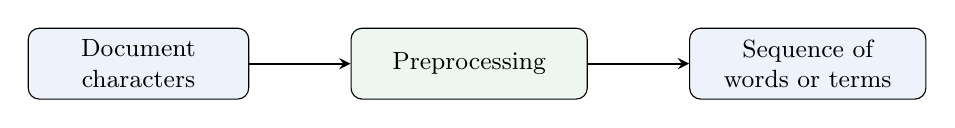
\begin{tikzpicture}[font=\small,>=stealth]
  \node[draw,rounded corners,fill=PlotBlue!8,align=center,
    minimum width=2.8cm,minimum height=0.9cm] (raw) at (0,0)
    {Document\\characters};
  \node[draw,rounded corners,fill=PlotGreen!8,align=center,
    minimum width=3cm,minimum height=0.9cm] (process) at (4.2,0)
    {Preprocessing};
  \node[draw,rounded corners,fill=PlotBlue!8,align=center,
    minimum width=3cm,minimum height=0.9cm] (terms) at (8.5,0)
    {Sequence of\\words or terms};
  \draw[->,thick] (raw.east) -- (process.west);
  \draw[->,thick] (process.east) -- (terms.west);
\end{tikzpicture}
\end{center}

\textbf{1. Tokenization.}
Split the text into units called \emph{tokens}. For example, the
document
\begin{center}
  ``Today is Monday and the weather is awesome.''
\end{center}
can be split into the word tokens
\begin{center}
  \texttt{Today}, \texttt{is}, \texttt{Monday}, \texttt{and},
  \texttt{the}, \texttt{weather}, \texttt{is}, \texttt{awesome}.
\end{center}
The input was a string of characters; the output is now a sequence
of separate terms.

\textbf{2. Stopword removal.}
Remove words on a chosen \emph{stopword list}, such as
\texttt{the}, \texttt{is}, \texttt{to} and \texttt{and}. These words
are often too common to help distinguish document topics. Depending
on the list, a phrase such as ``to be or not to be'' can lose most
of its words. We will later examine how common words affect cosine
similarity.

\textbf{3. Text normalization.}
Map different written forms to a common form when they should match.
For example,
\[
  \texttt{U.S.A.}\longrightarrow\texttt{USA},\qquad
  \texttt{Monday}\longrightarrow\texttt{monday}.
\]
The first transformation removes punctuation within an abbreviation;
the second ignores capitalization. Other choices concern accents
and hyphens. This normalization acts on the text; the vector
normalization introduced later rescales numerical coordinates.

\textbf{4. Stemming.}
Reduce related word forms to a common \emph{stem}, using rules that
remove affixes such as suffixes. For example,
\[
  \texttt{playing},\ \texttt{plays},\ \texttt{play}
  \quad\longrightarrow\quad\texttt{play}.
\]
The aim is to count these forms together instead of treating each
as a completely separate term. \texttt{NLTK} is a Python toolkit
for text-processing operations.

\section{From documents to vectors}

How can we turn a text into something on which we can perform
calculations? Suppose we want to find documents about similar topics.
Before choosing a distance or a similarity function, we need a numerical
representation of each document.

\begin{frameddefn}{Corpus and vocabulary}\label{def:corpus-vocabulary}
A \emph{corpus} is a collection of documents. Its \emph{vocabulary} is
the set of distinct terms appearing in those documents, after any
preprocessing. We fix an order for the vocabulary and use the same order
for every document.
\end{frameddefn}

\begin{framedexample}{Counting words in two documents}\label{ex:document-counts}
Consider the documents
\begin{align*}
  D_1&:\quad\text{``today we started at three''},\\
  D_2&:\quad\text{``we played three by three''}.
\end{align*}
For this example, we keep all the words. In the vocabulary order
\[
  (\texttt{at},\texttt{by},\texttt{played},\texttt{started},
    \texttt{three},\texttt{today},\texttt{we}),
\]
their word counts are
\begin{center}
\begin{tabular}{c|rrrrrrr}
  & \texttt{at} & \texttt{by} & \texttt{played} & \texttt{started}
  & \texttt{three} & \texttt{today} & \texttt{we}\\\hline
  $D_1$ & 1 & 0 & 0 & 1 & 1 & 1 & 1\\
  $D_2$ & 0 & 1 & 1 & 0 & 2 & 0 & 1
\end{tabular}
\end{center}
Each entry counts how many times a term occurs in a document. For
example, the entry for \texttt{three} in $D_2$ is $2$, because that word
appears twice. Reading the rows gives the vectors
\[
  \mathbf d_1=(1,0,0,1,1,1,1),\qquad
  \mathbf d_2=(0,1,1,0,2,0,1).
\]
The common coordinate order is essential: a coordinate must refer to
the same word in both documents for a comparison to make sense.
\end{framedexample}

\begin{frameddefn}{Count-vector representation}\label{def:document-vector}
Let the ordered vocabulary be $(t_1,\ldots,t_m)$. We represent document
$D_i$ by the vector $\mathbf d_i\in\mathbb R^m$, where
\[
  d_{ij}=\text{number of occurrences of term $t_j$ in document $D_i$}.
\]
Thus every term defines one coordinate, and every document becomes a
point in the same $m$-dimensional space. This is a basic
\emph{vector space model} of documents.
\end{frameddefn}

This representation records which terms occur and how often, but it
does not preserve their order in the text. Consequently, identical
count vectors do not necessarily imply identical meanings.

\section{Why document length can distort a comparison}

Now that documents are points, we can compare them using the $L_2$
distance already introduced in Definition~\ref{def:euclidean}.
For a two-dimensional illustration, keep only the coordinates
$(\texttt{three},\texttt{we})$ from Example~\ref{ex:document-counts}:
\[
  \mathbf u_1=(1,1),\qquad \mathbf u_2=(2,1).
\]
These are two-coordinate views of the documents, rather than their
complete vectors. Their distance is
\[
  \norm{\mathbf u_1-\mathbf u_2}_2
  =\sqrt{(1-2)^2+(1-1)^2}=1.
\]
We would like closeness between points to reflect similarity between
documents. However, raw word counts introduce a difficulty.

\begin{framedexample}{Repeating a document ten times}\label{ex:document-length}
Here $D_1$ is the original five-word document:
\[
  D_1:\quad\text{``today we started at three''}.
\]
Construct $D_3$ by repeating this \emph{entire sentence ten times
inside a single document}:
\[
  D_3:\quad\underbrace{\text{``today we started at three''}\;\cdots\;
    \text{``today we started at three''}}_{\text{10 copies of the sentence, 50 words in total}}.
\]
Using the same vocabulary order as before, compare the counts:
\begin{center}
\begin{tabular}{c|rrrrrrr}
  & \texttt{at} & \texttt{by} & \texttt{played} & \texttt{started}
  & \texttt{three} & \texttt{today} & \texttt{we}\\\hline
  $D_1$ & 1 & 0 & 0 & 1 & 1 & 1 & 1\\
  $D_3$ & 10 & 0 & 0 & 10 & 10 & 10 & 10
\end{tabular}
\end{center}
Thus $D_3$ is one longer document, not a collection of ten separate
documents. Every term now occurs ten times as often:
\[
  \mathbf d_3=10\mathbf d_1.
\]
In particular, \texttt{three} occurs ten times and \texttt{we} occurs
ten times, so the two-coordinate view becomes $\mathbf u_3=(10,10)$.
Its distance from the original is
\[
  \norm{\mathbf u_1-\mathbf u_3}_2
  =\sqrt{(1-10)^2+(1-10)^2}=9\sqrt2.
\]
Yet $D_3$ repeats exactly the same content: it adds no new information
and does not change the topic. Every word retains the same proportion
of the total text. The large distance is caused by the increase in
length, rather than by a change in word composition.
\end{framedexample}

\section{Removing the effect of length: normalization}

The idea is to rescale the counts so that multiplying every count by
the same factor does not change the representation. A first way to do
this is to divide each count by the total number of terms in the
document: we then compare \emph{relative frequencies}.

\begin{framedexample}{From counts to proportions}
As in Example~\ref{ex:document-length}, the documents are
\[
  D_1:\quad\text{``today we started at three''},
\]
\[
  D_3:\quad\underbrace{\text{``today we started at three''}\;\cdots\;
    \text{``today we started at three''}}_{\text{10 copies of the sentence, 50 words in total}}.
\]
\begin{center}
\begin{tabular}{c|rrrrrrr}
  & \texttt{at} & \texttt{by} & \texttt{played} & \texttt{started}
  & \texttt{three} & \texttt{today} & \texttt{we}\\\hline
  $D_1$ & 1 & 0 & 0 & 1 & 1 & 1 & 1\\
  $D_3$ & 10 & 0 & 0 & 10 & 10 & 10 & 10
\end{tabular}
\end{center}
Document $D_1$ contains five words and $D_3$ contains fifty. For the
coordinates $(\texttt{three},\texttt{we})$, dividing by the respective
document lengths gives
\[
  D_1:\quad\left(\frac15,\frac15\right)=(0.2,0.2),\qquad
  D_3:\quad\left(\frac{10}{50},\frac{10}{50}\right)=(0.2,0.2).
\]
The representations now agree. Notice that the denominators count
\emph{all} the terms in each document, not just the two displayed
coordinates.
\end{framedexample}

More generally, we can divide a nonzero document vector by its norm.
\begin{frameddefn}{Document-vector normalization}\label{def:document-normalization}
For a nonzero vector $\mathbf d$ and a chosen norm, its normalized
version is
\[
  \widehat{\mathbf d}=\frac{\mathbf d}{\norm{\mathbf d}}.
\]
Each coordinate is divided by the same positive number, and the
resulting vector has norm $1$.
\end{frameddefn}

For a complete vector of nonnegative term counts, the $L_1$ norm is
the sum of all counts, hence the total number of terms counted in the
document. Normalizing with $L_1$ therefore gives the relative
frequencies used above. Normalizing with $L_2$ instead gives a vector
of Euclidean norm $1$; these are two different choices of scale.

Both choices remove a uniform multiplication of the counts. Indeed,
for $c>0$ and $\mathbf d\neq\mathbf0$,
\[
  \frac{c\mathbf d}{\norm{c\mathbf d}}
  =\frac{c\mathbf d}{c\norm{\mathbf d}}
  =\frac{\mathbf d}{\norm{\mathbf d}}.
\]
Thus repeating $D_1$ ten times yields the same normalized vector.
Geometrically, normalization rescales the vector without changing its
direction. A document with no counted terms has the zero vector and
cannot be normalized by this formula.

\section{Comparing directions: cosine similarity}

Normalization suggests a geometric way to compare documents: two
vectors can have different lengths while pointing in the same direction.
Now, we can consider another idea: compare the \emph{angle} between
the vectors. If their counts are proportional, their relative word
composition is the same and the angle is zero.

\begin{framedexample}{Same direction, different lengths}
As before, keep only the coordinates $(\texttt{three},\texttt{we})$:
\[
  \mathbf u_1=(1,1),\qquad \mathbf u_3=(10,10).
\]
Draw each vector as an arrow starting at the origin. The arrow for
$\mathbf u_3$ is ten times as long, but points in exactly the same
direction as $\mathbf u_1$: the angle between them is $0^\circ$.
Now consider $\mathbf u_2=(2,1)$. Here \texttt{three} occurs twice as
often as \texttt{we}, so its arrow points more towards the
\texttt{three} axis and forms a positive angle with $\mathbf u_1$.
\begin{center}
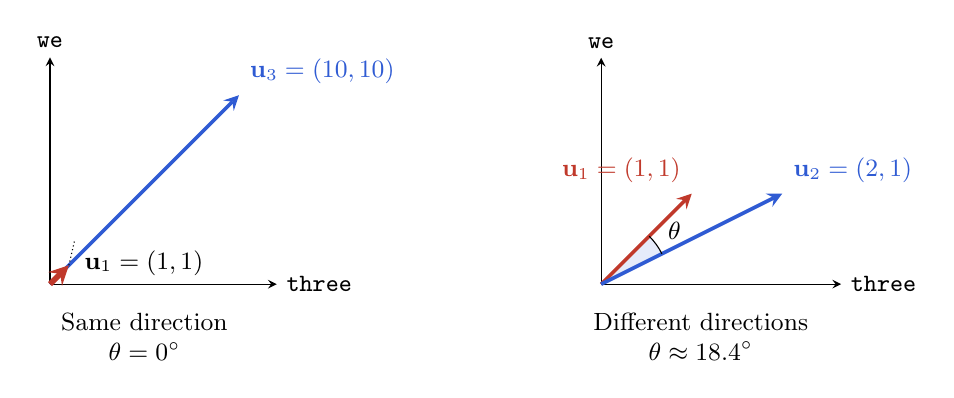
\begin{tikzpicture}[>=stealth,font=\small]
  \begin{scope}[scale=0.24]
    \draw[->] (0,0) -- (12,0) node[right] {\texttt{three}};
    \draw[->] (0,0) -- (0,12) node[above] {\texttt{we}};
    \draw[->,PlotBlue,line width=1.3pt] (0,0) -- (10,10)
      node[above right] {$\mathbf u_3=(10,10)$};
    \draw[->,PlotRed,line width=2pt] (0,0) -- (1,1);
    \node[anchor=north west] at (1.3,2.3) {$\mathbf u_1=(1,1)$};
    \draw[densely dotted] (1,1) -- (1.3,2.3);
    \node[align=center] at (5,-2.8) {Same direction\\$\theta=0^\circ$};
  \end{scope}
  \begin{scope}[xshift=7cm,scale=1.15]
    \draw[->] (0,0) -- (2.65,0) node[right] {\texttt{three}};
    \draw[->] (0,0) -- (0,2.5) node[above] {\texttt{we}};
    \fill[PlotBlue!12] (0,0) -- (26.565:0.75)
      arc[start angle=26.565,end angle=45,radius=0.75] -- cycle;
    \draw[->,PlotRed,line width=1.3pt] (0,0) -- (1,1)
      node[above left] {$\mathbf u_1=(1,1)$};
    \draw[->,PlotBlue,line width=1.3pt] (0,0) -- (2,1)
      node[above right] {$\mathbf u_2=(2,1)$};
    \draw (26.565:0.75) arc[start angle=26.565,end angle=45,radius=0.75];
    \node at (35.8:1) {$\theta$};
    \node[align=center] at (1.1,-0.58) {Different directions\\$\theta\approx18.4^\circ$};
  \end{scope}
\end{tikzpicture}
\end{center}
\end{framedexample}

The smaller the angle, the more similar the proportions of terms in
the two vectors. We turn this idea into a numerical similarity by
taking the cosine of that angle.

\begin{frameddefn}{Cosine similarity}\label{def:cosine-similarity}
For two nonzero document vectors $\mathbf u$ and $\mathbf v$, let
$\theta$ be the angle between them. Their \emph{cosine similarity} is
\[
  \operatorname{sim}_{\cos}(\mathbf u,\mathbf v)=\cos\theta.
\]
\end{frameddefn}

For nonnegative count vectors, the angle lies between $0^\circ$ and
$90^\circ$, so the similarity lies between $0$ and $1$:
\begin{itemize}
  \item At $0^\circ$, the similarity is $1$: the vectors point in the
    same direction, and their counts are proportional.
  \item Between $0^\circ$ and $90^\circ$, the similarity lies strictly
    between $1$ and $0$. As the angle increases, the similarity decreases.
  \item At $90^\circ$, the similarity is $0$: there is no coordinate
    with a positive count in both vectors. For complete document
    vectors, this means that the documents share no counted terms.
\end{itemize}
In particular, $D_1$ and its tenfold repetition $D_3$ have cosine
similarity $1$. This measures similarity of word composition; as with
the count representation itself, it does not capture word order or
guarantee identical meanings. A zero vector has no direction, so the
similarity above is not defined for an empty count vector.

\subsection{Computing cosine similarity from coordinates}

We do not need to measure the angle first. For two nonzero vectors
$\mathbf u,\mathbf v\in\mathbb R^m$, we can compute its cosine directly
from their coordinates:
\[
  \operatorname{sim}_{\cos}(\mathbf u,\mathbf v)
  =\frac{\mathbf u\cdot\mathbf v}{\norm{\mathbf u}_2\norm{\mathbf v}_2}
  =\frac{\sum_{j=1}^{m}u_jv_j}
    {\sqrt{\sum_{j=1}^{m}u_j^2}\sqrt{\sum_{j=1}^{m}v_j^2}}.
\]
The numerator is the \emph{dot product}: multiply corresponding
coordinates, then add the results. The denominator is the product of
the two $L_2$ norms.

\begin{framedexample}{Computing the similarity step by step}
Take the two vectors from the right-hand graph, in the coordinate order
$(\texttt{three},\texttt{we})$:
\[
  \mathbf u_1=(1,1),\qquad\mathbf u_2=(2,1).
\]
\textbf{Step 1: compute the dot product.}
Multiply the counts for the same word and add:
\[
  \mathbf u_1\cdot\mathbf u_2
  =\underbrace{1\cdot2}_{\texttt{three}}
   +\underbrace{1\cdot1}_{\texttt{we}}=3.
\]
Each term compares the count of one word in the first document with
the count of that same word in the second.

\textbf{Step 2: compute the two $L_2$ norms.}
\[
  \norm{\mathbf u_1}_2=\sqrt{1^2+1^2}=\sqrt2,\qquad
  \norm{\mathbf u_2}_2=\sqrt{2^2+1^2}=\sqrt5.
\]
\textbf{Step 3: divide the dot product by the product of the norms.}
\[
  \operatorname{sim}_{\cos}(\mathbf u_1,\mathbf u_2)
  =\frac{3}{\sqrt2\sqrt5}
  =\frac{3}{\sqrt{10}}\approx0.949.
\]
The result is close to $1$: the vectors point in similar directions,
although their word proportions differ. This is the cosine of the
angle of approximately $18.4^\circ$ shown in the graph.
\end{framedexample}

\subsection{A limitation: matching words is not understanding meaning}

Two texts can discuss the same subject while using different terms,
such as \texttt{cat} and \texttt{feline}. In our representation these
are separate coordinates: a shared meaning does not create a shared
term. Conversely, the same word can have different meanings in
different contexts. The count-based model does not resolve these
ambiguities by itself. The next weighting step changes the importance
of terms, but does not make distinct synonyms the same coordinate.

\section{Why some words should count more than others}

We can now compare documents using cosine similarity. However, in
the count representation every occurrence has the same weight,
regardless of which word it belongs to. A common word can therefore
create a similarity that tells us little about the documents' topics.

\begin{framedexample}{A similarity caused by a common word}
Consider two short documents:
\[
  D_A:\quad\text{``the cat''},\qquad
  D_B:\quad\text{``the dog''}.
\]
Using the vocabulary order $(\texttt{the},\texttt{cat},\texttt{dog})$,
we obtain
\[
  \mathbf d_A=(1,1,0),\qquad\mathbf d_B=(1,0,1).
\]
Their dot product is
\[
  \mathbf d_A\cdot\mathbf d_B
  =\underbrace{1\cdot1}_{\texttt{the}}
   +\underbrace{1\cdot0}_{\texttt{cat}}
   +\underbrace{0\cdot1}_{\texttt{dog}}=1.
\]
Both vectors have $L_2$ norm $\sqrt2$, so
\[
  \operatorname{sim}_{\cos}(\mathbf d_A,\mathbf d_B)
  =\frac{1}{\sqrt2\sqrt2}=\frac12.
\]
The similarity comes entirely from \texttt{the}, a word that provides
little information about what these documents discuss.
\end{framedexample}

A first solution is to remove \emph{stopwords}: very common words,
such as articles and prepositions, that are often uninformative for
the comparison. In the example, removing \texttt{the} leaves
\[
  D_A:\quad\text{``cat''},\qquad D_B:\quad\text{``dog''}.
\]
With the vocabulary order $(\texttt{cat},\texttt{dog})$, the vectors
become
\[
  \mathbf d_A=(1,0),\qquad\mathbf d_B=(0,1).
\]
Their dot product is zero and both norms are $1$, so their cosine
similarity is now $0$: they share no remaining terms.

This suggests a more general idea: words are not all equally
informative. Instead of only removing certain words, we can assign
different weights to the terms, so that informative words contribute
more to the comparison.

\section{Weighting terms by their rarity: IDF}

A word that appears in almost every document does little to distinguish
documents from one another. A word found in only a few documents can
be more characteristic. For example, in a corpus of cooking texts,
\texttt{food} might occur almost everywhere, whereas \texttt{guanciale}
might appear only in recipes using that ingredient.

\begin{framedexample}{Counting documents rather than occurrences}
Suppose our corpus contains $100$ documents:
\begin{center}
\begin{tabular}{l|r}
  Term & Documents containing the term\\\hline
  \texttt{food} & 100\\
  \texttt{pasta} & 20\\
  \texttt{guanciale} & 2
\end{tabular}
\end{center}
These are counts of \emph{documents}, not occurrences. If
\texttt{guanciale} occurs ten times in one recipe, that recipe still
contributes only $1$ to the count of documents containing the term.
\end{framedexample}

\textbf{Step 1: count the documents containing each term.}
Let $N$ be the total number of documents. For a term $t$, write
$\operatorname{df}(t)$ for its \emph{document frequency}: the number
of documents containing it.

\textbf{Step 2: compare the total with that count.}
Consider the ratio $N/\operatorname{df}(t)$. In our example,
\[
  \texttt{food}:\ \frac{100}{100}=1,\qquad
  \texttt{pasta}:\ \frac{100}{20}=5,\qquad
  \texttt{guanciale}:\ \frac{100}{2}=50.
\]
The rarer the term in the corpus, the larger this ratio.

\textbf{Step 3: take the logarithm of the ratio.}
The logarithm reduces the differences between the weights while
preserving their order: rarer terms still receive larger weights.

\begin{frameddefn}{Inverse document frequency}\label{def:idf}
For a term $t$ appearing in at least one document of a corpus of $N$
documents, its \emph{inverse document frequency} is
\[
  \operatorname{IDF}(t)
  =\log\left(\frac{N}{\operatorname{df}(t)}\right),
\]
where $\operatorname{df}(t)$ is the number of documents containing $t$.
\end{frameddefn}

\begin{framedexample}{IDF weights for the cooking corpus}
Using base-$10$ logarithms, the weights are
\begin{center}
\begin{tabular}{l|c|c}
  Term & $N/\operatorname{df}(t)$ & $\operatorname{IDF}(t)$\\\hline
  \texttt{food} & $100/100=1$ & $\log_{10}(1)=0$\\
  \texttt{pasta} & $100/20=5$ & $\log_{10}(5)\approx0.699$\\
  \texttt{guanciale} & $100/2=50$ & $\log_{10}(50)\approx1.699$
\end{tabular}
\end{center}
Thus \texttt{guanciale} receives more weight than \texttt{pasta}.
The word \texttt{food}, present in every document, receives weight
$0$: under this formula it provides no information for distinguishing
the documents in this corpus.
\end{framedexample}

\section{Combining term frequency and rarity: TF-IDF}

We now combine two pieces of information. The \emph{term frequency}
(TF) describes how often a term occurs in one particular document;
IDF describes how rare that term is across the entire corpus. Here
we use the raw occurrence count as TF, consistently with our count
vectors.

\begin{frameddefn}{TF-IDF weight}\label{def:tf-idf}
Let $\operatorname{TF}(t,D)$ be the number of occurrences of term $t$
in document $D$. Its \emph{TF-IDF weight} is
\[
  \operatorname{TF\!\text{-}\!IDF}(t,D)
  =\operatorname{TF}(t,D)\cdot\operatorname{IDF}(t).
\]
\end{frameddefn}

\begin{framedexample}{From counts to TF-IDF weights}
\textbf{Step 1: keep the same corpus of $100$ documents.}
Using the base-$10$ logarithms from the previous example,
\[
  \operatorname{IDF}(\texttt{food})=0,\qquad
  \operatorname{IDF}(\texttt{pasta})\approx0.699,\qquad
  \operatorname{IDF}(\texttt{guanciale})\approx1.699.
\]
\textbf{Step 2: choose a document $D$ in this corpus.}
Suppose its counts for these terms are
\begin{center}
\begin{tabular}{l|r}
  Term & TF in document $D$\\\hline
  \texttt{food} & 4\\
  \texttt{pasta} & 3\\
  \texttt{guanciale} & 2
\end{tabular}
\end{center}
In the coordinate order
$(\texttt{food},\texttt{pasta},\texttt{guanciale})$, the corresponding
count vector is $\mathbf d=(4,3,2)$. These are the three coordinates
we are following in the example.

\textbf{Step 3: multiply each count by its term's IDF.}
\begin{center}
\begin{tabular}{l|r|r|l}
  Term & TF & IDF & TF-IDF\\\hline
  \texttt{food} & 4 & 0 & $4\cdot0=0$\\
  \texttt{pasta} & 3 & $\approx0.699$ & $3\log_{10}(5)\approx2.097$\\
  \texttt{guanciale} & 2 & $\approx1.699$ & $2\log_{10}(50)\approx3.398$
\end{tabular}
\end{center}
The weighted vector is therefore
\[
  \mathbf d_{\text{TF-IDF}}\approx(0,\;2.097,\;3.398).
\]
Although \texttt{guanciale} occurs less often than \texttt{pasta} in
this document, it receives a larger weight because it is rarer in
the corpus. The term \texttt{food} receives weight zero because it
appears in every document.
\end{framedexample}

TF depends on the particular document being represented. IDF depends
on the corpus: for a fixed corpus, a term has the same IDF in every
document. We can then compare the weighted document vectors using
the same cosine-similarity formula as before, provided neither
weighted vector is zero.

\section{Using document vectors for search}\label{sec:vector-search}

We can use \hyperref[def:tf-idf]{TF-IDF} vectors to build a search engine. A \emph{query} is
the text entered by the user. Given a query and a positive integer
$k$, our goal is to return the $k$ documents most similar to that
query (or all documents if the corpus contains fewer than $k$).
For example, $k=3$ asks for the three highest-scoring results.

The first step is to represent the query as a vector in the
\emph{same space} as the documents: the same vocabulary, the same
coordinate order and the same IDF weights.

\begin{framedexample}{Turning a query into a vector}
Suppose the user searches for
\[
  Q:\quad\text{``pasta guanciale''}.
\]
Keep the coordinate order
$(\texttt{food},\texttt{pasta},\texttt{guanciale})$ from the cooking
example.

\textbf{Step 1: count the query terms.}
The query contains no occurrence of \texttt{food}, one occurrence of
\texttt{pasta} and one of \texttt{guanciale}. Its count vector is
\[
  \mathbf q_{\text{counts}}=(0,1,1).
\]
\textbf{Step 2: apply the same IDF weights as for the documents.}
Use the IDF values already computed from the corpus, rather than
recomputing IDF from the query:
\[
  \mathbf q_{\text{TF-IDF}}
  \approx(0\cdot0,\;1\cdot0.699,\;1\cdot1.699)
  =(0,\;0.699,\;1.699).
\]
As before, we display the three coordinates being followed in this
example; any other vocabulary terms absent from the query have
coordinate zero.

\textbf{Step 3: compare the query with each document.}
For each document $D_i$, assign the score
\[
  \operatorname{score}(D_i)
  =\operatorname{sim}_{\cos}
    \bigl(\mathbf q_{\text{TF-IDF}},\mathbf d_{i,\text{TF-IDF}}\bigr).
\]
Here both vectors use the full common vocabulary and are assumed to
be nonzero. A higher score means that the document's direction is
closer to the query's direction. Sort the documents by decreasing
score and return the first $k$.
\end{framedexample}

The query is therefore treated as a small document. Representing it
with the same coordinates and corpus-based IDF weights lets us use
the same cosine-similarity calculation for retrieval.

\subsection{The cost of searching every document}\label{sec:search-all-cost}

The simplest search procedure follows four steps:
\begin{enumerate}
  \item Compute cosine similarity between the query and every document.
  \item Store each document's score.
  \item Sort the documents by decreasing score.
  \item Return the first $k$ results.
\end{enumerate}
Suppose the corpus contains $N$ documents and the vocabulary contains
$m$ terms. We analyse the direct implementation that scans all $m$
coordinates of each document vector.

\textbf{First cost: computing all scores.}
Each vector has $m$ coordinates. Scanning all of them to compare the
query with one document takes $\Theta(m)$ time. Repeating this for
all $N$ documents takes
\[
  \Theta(Nm).
\]
\begin{framedexample}{A large corpus}
With one million documents and a vocabulary of one hundred thousand
terms, the direct implementation examines
\[
  10^6\cdot10^5=10^{11}
\]
pairs of coordinates for every query. Each pair contains the query
weight and the document weight for the same vocabulary term.
\end{framedexample}

\textbf{Second cost: sorting the scores.}
One simple approach repeatedly finds the largest remaining score,
places its document next in the ordering and removes it from
consideration. Producing the complete ordering this way scans
\[
  N+(N-1)+\cdots+1=\frac{N(N+1)}2
\]
scores, so it takes $\Theta(N^2)$ time.

An efficient comparison-based sorting algorithm sorts the $N$ scores
in $O(N\log N)$ time. Thus computing all scores and sorting them gives
the overall bound
\[
  O(Nm+N\log N).
\]
This procedure works, but repeats substantial work whenever a new
query arrives. The next question is which work can be performed once,
while preparing the documents, and which must wait until the query
is known.

\subsection{Preparing the corpus offline, answering queries online}

The corpus is usually available before the user submits a query.
We can therefore prepare information about the documents in advance,
instead of repeating all the preparation for every search.

\begin{frameddefn}{Offline and online phases}\label{def:offline-online}
The \emph{offline phase} processes the corpus before a particular query
is known, storing information useful for future searches. The
\emph{online phase} starts when a query arrives and uses that stored
information to compute the results.
\end{frameddefn}

Here ``offline'' means independent of the current query, rather than
disconnected from the Internet. For our vector-based search, we can
prepare the vocabulary, document counts, IDF weights and document
TF-IDF vectors offline. We can also store their $L_2$ norms, or their
normalized vectors. Online, we process the query, construct its vector
using the stored vocabulary and IDF, and compute the results.

\begin{framedexample}{Many users searching the same corpus}
Suppose one user searches for ``pasta guanciale'' and another for
``tomato restaurant''. Their query vectors differ, but the document
vectors and corpus-based IDF weights are the same. We prepare those
once and reuse them for both searches. If the corpus changes, the
stored information must be updated as appropriate.
\end{framedexample}

Precomputing document vectors saves preparation work, but scanning
every document still has a cost. To understand how a different data
organization can help, we now consider a Boolean version of search.

\section{Boolean AND search}

Suppose the query is ``pasta guanciale''. This time we want every
document containing \emph{both} words. A document containing only
\texttt{pasta} does not qualify, however often that word occurs.

\begin{frameddefn}{Boolean AND query}\label{def:boolean-and}
Represent each document $D_i$ by its set of terms $T_i$, and let $Q$
be a nonempty set of query terms. A Boolean AND query returns
\[
  R(Q)=\{i:Q\subseteq T_i\}.
\]
Thus a document qualifies precisely when it contains every query term.
\end{frameddefn}

This search asks a membership question, rather than assigning cosine
scores and selecting the top $k$. Its output is the set of all
qualifying document identifiers.

\subsection{A direct scan}

A first approach to answering this query is to visit each document,
check whether it contains every query term, and add its identifier
to the result if it does.
For a large corpus this inspects many documents that contain none of
the query terms. We would like to find the relevant documents without
starting a new scan of the entire corpus each time.

\section{The inverted index}

The usual document representation answers: ``Which terms occur in
this document?'' We now reverse the direction and store the answer
to: ``Which documents contain this term?''

\begin{frameddefn}{Inverted index and posting list}\label{def:inverted-index}
An \emph{inverted index} maps each term $t$ to its \emph{posting list}
$L(t)$: the sorted list of identifiers of documents containing $t$.
Each document identifier appears at most once in a term's list,
regardless of how often that term occurs in the document.
\end{frameddefn}

\begin{framedexample}{Building the index from six documents}\label{ex:inverted-index}
Use letters to represent terms, and number the documents from $1$ to
$6$. The original representation is
\begin{center}
\begin{tabular}{c|l}
  Document identifier & Terms in the document\\\hline
  $1$ & $A,B,C,D$\\
  $2$ & $A,B,E,G$\\
  $3$ & $B,D,F$\\
  $4$ & $A,C,D,E$\\
  $5$ & $A,C,G$\\
  $6$ & $C,D,G$
\end{tabular}
\end{center}
\textbf{Step 1: collect the documents containing $A$.}
Reading the table, $A$ occurs in documents $1,2,4,5$, so
$L(A)=[1,2,4,5]$.

\textbf{Step 2: repeat for every term.}
The complete inverted index for these six documents is
\begin{center}
\begin{tabular}{c|l}
  Term & Posting list\\\hline
  $A$ & $[1,2,4,5]$\\
  $B$ & $[1,2,3]$\\
  $C$ & $[1,4,5,6]$\\
  $D$ & $[1,3,4,6]$\\
  $E$ & $[2,4]$\\
  $F$ & $[3]$\\
  $G$ & $[2,5,6]$
\end{tabular}
\end{center}
For a single-term query $E$, the answer is immediately $\{2,4\}$.
We look up $L(E)$ rather than checking all six documents.
\end{framedexample}

We build the inverted index offline. One way is to process documents
in increasing identifier order and append each identifier to the
lists of its distinct terms; the lists are then already sorted.
Online, a query only needs the lists for its own terms.

\subsection{AND means intersecting posting lists}

For the query $Q=\{A,C,E\}$, a document must occur in all three lists:
\[
  R(Q)=L(A)\cap L(C)\cap L(E).
\]
Here we use intersection to mean the identifiers shared by the lists.
Using Example~\ref{ex:inverted-index},
\[
  \{1,2,4,5\}\cap\{1,4,5,6\}=\{1,4,5\},
  \qquad \{1,4,5\}\cap\{2,4\}=\{4\}.
\]
The answer is document $4$. Looking back at its row confirms that it
contains $A,C,E$. If any query term has no posting list, no document
contains that term and the AND result is empty.

\section{Intersecting sorted lists with pointers}

How can we find the intersection without repeatedly searching one
list for every element of another? Sorting lets us move through the
lists from left to right, using a \emph{pointer} to mark the current
position in each list.

\begin{framedexample}{Following the pointers}\label{ex:posting-pointers}
The query is $Q=\{A,C,E\}$: we want documents containing all three
terms. The posting lists are
\[
  L(A)=[1,2,4,5],\quad L(C)=[1,4,5,6],\quad L(E)=[2,4].
\]
Each number identifies a document. Put a pointer at the first element
of each list; the boxed entries below show the current positions.

\textbf{Step 1: the pointers read $1,1,2$.}
\[
\begin{aligned}
  L(A)&=[\boxed{1},2,4,5],\\
  L(C)&=[\boxed{1},4,5,6],\\
  L(E)&=[\boxed{2},4].
\end{aligned}
\]
Document $1$ contains $A$ and $C$, but not $E$. In $L(E)$ we are
already at $2$; since the list is sorted, no later entry can be $1$.
Thus $1$ cannot be a result. Advance the two pointers reading $1$
(those in $L(A)$ and $L(C)$), leaving the pointer in $L(E)$ at $2$.

\textbf{Step 2: the pointers now read $2,4,2$.}
\[
\begin{aligned}
  L(A)&=[1,\boxed{2},4,5],\\
  L(C)&=[1,\boxed{4},5,6],\\
  L(E)&=[\boxed{2},4].
\end{aligned}
\]
Document $2$ contains $A$ and $E$, but not $C$. In $L(C)$ we are
already at $4$, so we cannot find $2$ further along that list.
Discard $2$: advance the pointers in $L(A)$ and $L(E)$, leaving the
pointer in $L(C)$ at $4$.

\textbf{Step 3: the pointers now read $4,4,4$.}
\[
\begin{aligned}
  L(A)&=[1,2,\boxed{4},5],\\
  L(C)&=[1,\boxed{4},5,6],\\
  L(E)&=[2,\boxed{4}].
\end{aligned}
\]
All three pointers read the same identifier: document $4$ contains
$A$, $C$ and $E$. Add it to the result, giving $R=[4]$, then advance
all three pointers.

\textbf{Step 4: the list for $E$ is exhausted.}
\[
\begin{aligned}
  L(A)&=[1,2,4,\boxed{5}],\\
  L(C)&=[1,4,\boxed{5},6],\\
  L(E)&=[2,4]\quad\text{(pointer past the last entry)}.
\end{aligned}
\]
The other pointers read $5$, but $L(E)$ has no entries left. No
further identifier can occur in all three lists, so we stop. The
final result is $R=[4]$: return document $D_4$.

\textbf{Summary of the pointer movements.}
\begin{center}
\begin{tabular}{c|ccc|l}
  Step & $L(A)$ & $L(C)$ & $L(E)$ & Action\\\hline
  $1$ & $1$ & $1$ & $2$ & Advance the pointers at $1$.\\
  $2$ & $2$ & $4$ & $2$ & Advance the pointers at $2$.\\
  $3$ & $4$ & $4$ & $4$ & Output $4$; advance all three.\\
  $4$ & $5$ & $5$ & exhausted & Stop.
\end{tabular}
\end{center}
\end{framedexample}

For a fixed small number of lists, this gives a simple rule: if all
current identifiers agree, output that identifier and advance every
pointer; otherwise advance the pointers at the smallest current
identifier. No pointer needs to move backwards.

\subsection{A two-list intersection algorithm}

For two lists, there are only three cases: the current identifiers
are equal, the left one is smaller, or the right one is smaller.
The following algorithm makes each case explicit.

\Needspace{20\baselineskip}
\begin{framedalgo}{Intersect two sorted posting lists}\label{alg:posting-intersection}
\begin{algorithmic}[1]
  \Function{Intersect}{$L,M$}
    \State $i\gets1$, $j\gets1$, $R\gets[\,]$
    \While{$i\leq\abs L$ and $j\leq\abs M$}
      \If{$L[i]=M[j]$}
        \State Append $L[i]$ to $R$
        \State $i\gets i+1$, $j\gets j+1$
      \ElsIf{$L[i]<M[j]$}
        \State $i\gets i+1$
      \Else
        \State $j\gets j+1$
      \EndIf
    \EndWhile
    \State \Return $R$
  \EndFunction
\end{algorithmic}
\end{framedalgo}

Every iteration advances at least one pointer, and each pointer
crosses its list at most once. Thus intersecting lists of lengths
$a$ and $b$ takes $O(a+b)$ time, with $\Theta(a+b)$ in the worst case.
It can finish sooner if one list is exhausted early.

\subsection{Query cost: the lengths of the relevant lists}

We now measure the work needed to answer a query after the inverted
index has already been built. Let $n_t=\abs{L(t)}$ be the length of
the \hyperref[def:inverted-index]{posting list} for query term $t$:
the number of documents containing that term. We work with the lists
selected by the query.

For several terms, we can apply the two-list algorithm repeatedly.
Start with the shortest posting list and intersect the current
result with each of the other lists. Stop if the result becomes empty.

\begin{framedexample}{The cost of a three-term query}
Take $Q=\{A,C,E\}$, with
\[
  L(A)=[1,2,4,5],\quad L(C)=[1,4,5,6],\quad L(E)=[2,4].
\]
\textbf{Step 1: count the lengths of the relevant lists.}
\begin{center}
\begin{tabular}{c|c}
  Term & Posting-list length\\\hline
  $A$ & $n_A=4$\\
  $C$ & $n_C=4$\\
  $E$ & $n_E=2$
\end{tabular}
\end{center}
Their sum is $n_A+n_C+n_E=4+4+2=10$. The lists for $B,D,F,G$ are
not needed for this query.

\textbf{Step 2: start with the shortest list, $L(E)$, and intersect it
with $L(A)$.}
\[
  [2,4]\cap[1,2,4,5]=[2,4].
\]
The pairs of current identifiers compared by the two pointers are
\[
  (2,1)\ \longrightarrow\ (2,2)\ \longrightarrow\ (4,4).
\]
First advance past $1$ in $L(A)$. Then output $2$ and advance both
pointers; next output $4$ and advance both again. The first list is
now exhausted. We made three comparisons and obtained $R=[2,4]$.

\textbf{Step 3: intersect the intermediate result with $L(C)$.}
\[
  [2,4]\cap[1,4,5,6]=[4].
\]
This time the comparisons are
\[
  (2,1)\ \longrightarrow\ (2,4)\ \longrightarrow\ (4,4).
\]
Advance past $1$ in $L(C)$, then past $2$ in the intermediate
result. Finally output $4$ and advance both pointers. The intermediate
list is exhausted. These are three more comparisons, and the final
answer is document $D_4$.

\textbf{Step 4: relate the work to the list lengths.}
The first intersection has the bound $O(2+4)$; the second also has
the bound $O(2+4)$. The intermediate list never grows: it starts with
at most two identifiers and intersections can only remove them.
We performed six identifier comparisons in this example.

The general bound below is proportional to the sum of the original
posting-list lengths, which here is $10$.
\end{framedexample}

\textbf{Why starting with the shortest list gives the total bound.}
The intermediate result is always a subset of the shortest initial
list, so its length never exceeds that list's length.

Let $s$ be the length of the shortest initial list and $n_t$ the
length of the next posting list. The intermediate result has length
at most $s$, so intersecting it with that next list costs $O(s+n_t)$.
Since the next list cannot be shorter than the shortest initial list,
$s\leq n_t$. Therefore
\[
  s+n_t\leq2n_t,\qquad O(s+n_t)=O(n_t).
\]

\Needspace{14\baselineskip}
To see the total bound, let $r=\abs Q$, the number of query terms
and hence the number of posting lists. One list is used as the
starting point, leaving $r-1$ lists to intersect with the current
result. Since each of these other lists has length at least $s$,
\[
  (r-1)s\leq\sum_{t\in Q\setminus\{t_*\}}n_t,
\]
where $t_*$ is the term with the shortest list. Consequently the
total intersection time is
\[
  O\left(\sum_{t\in Q}n_t\right).
\]
To retrieve the lists, look up each of the $r$ query terms in the
inverted index. With a hash-table dictionary, each lookup takes
$O(1)$ expected time, giving $O(r)$ expected time for all lookups.
Retrieving a list here means obtaining a reference to the stored
list, rather than copying or scanning its entries. Scanning the
entries is counted in the intersection cost.
The overall expected query cost is therefore
\[
  \boxed{O\left(
    \underbrace{r}_{\text{retrieve the lists}}
    +\underbrace{\sum_{t\in Q}n_t}_{\text{intersect the lists}}
  \right)}.
\]
In a much larger corpus, rare query terms can have short lists,
making the online search far cheaper than a full corpus scan.
If the terms occur in almost every document, their lists are long
and the advantage is smaller.

\lecturestart{22 October}

\section{Terms as integer identifiers}

Comparing numbers is simpler and cheaper than comparing words.
Offline, we can sort the vocabulary and give each term an integer
\emph{identifier}, its position in that order. A document is then
stored as a sequence of identifiers, and the inverted index uses
these numbers as keys.

\begin{framedexample}{From words to identifiers}
In a sorted English vocabulary, \texttt{a} receives $0$, \texttt{aa}
receives $1$, and so on. Suppose \texttt{is}, \texttt{thursday} and
\texttt{today} receive the identifiers below.
\begin{center}
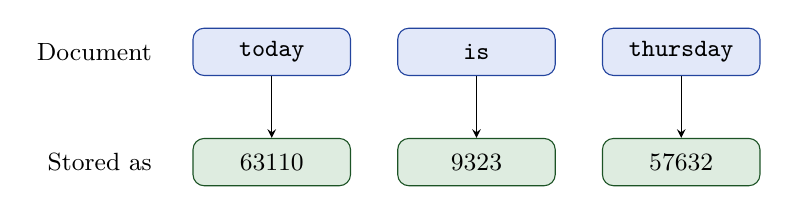
\begin{tikzpicture}[>=stealth,font=\small,
  word/.style={draw=PlotBlue!75!black,rounded corners,fill=PlotBlue!14,
    minimum width=2cm,minimum height=0.6cm},
  termid/.style={draw=PlotGreen!60!black,rounded corners,fill=PlotGreen!16,
    minimum width=2cm,minimum height=0.6cm}]
  \node[anchor=east] at (-1.4,0) {Document};
  \node[anchor=east] at (-1.4,-1.4) {Stored as};
  \foreach \x/\w/\n in {0/today/63110,2.6/is/9323,5.2/thursday/57632} {
    \node[word] (w\n) at (\x,0) {\texttt{\w}};
    \node[termid] (i\n) at (\x,-1.4) {$\n$};
    \draw[->] (w\n) -- (i\n);
  }
\end{tikzpicture}
\end{center}
\end{framedexample}

In the examples we keep letters such as $A,B,C$ for the terms, which
are easier to read than five-digit numbers.

\section{Boolean queries with OR and NOT}

An AND query intersects posting lists. A Boolean query can also use
OR and NOT. For example, someone looking for fettuccine with veal,
but not fettuccine Alfredo, could search for
\begin{center}
  \texttt{fettuccine} AND \texttt{vitello} AND NOT \texttt{alfredo}.
\end{center}
For two posting lists $L$ and $M$, each operation corresponds to a
set operation on document identifiers:
\begin{center}
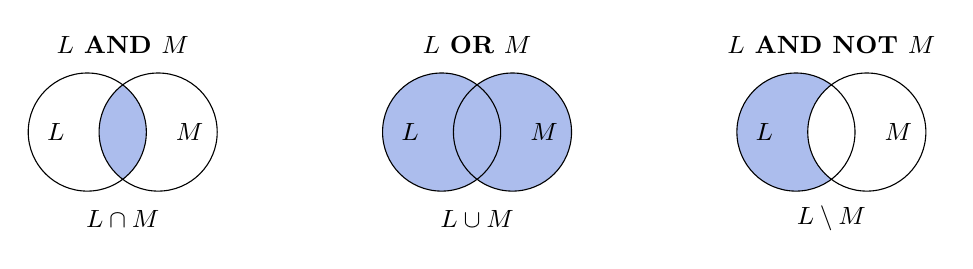
\begin{tikzpicture}[font=\small]
  % L AND M: the overlap.
  \begin{scope}
    \clip (-0.45,0) circle (0.75);
    \fill[PlotBlue!40] (0.45,0) circle (0.75);
  \end{scope}
  % L OR M: both circles.
  \fill[PlotBlue!40] (4.05,0) circle (0.75) (4.95,0) circle (0.75);
  % L AND NOT M: L without the overlap.
  \begin{scope}
    \clip (8.55,0) circle (0.75);
    \fill[PlotBlue!40,even odd rule] (8.55,0) circle (0.75)
      (9.45,0) circle (0.75);
  \end{scope}
  \foreach \x/\op/\set in {0/AND/{L\cap M},4.5/OR/{L\cup M},
      9/AND NOT/{L\setminus M}} {
    \draw (\x-0.45,0) circle (0.75) (\x+0.45,0) circle (0.75);
    \node at (\x-0.85,0) {$L$};
    \node at (\x+0.85,0) {$M$};
    \node[font=\small\bfseries] at (\x,1.1) {$L$ \op\ $M$};
    \node at (\x,-1.1) {$\set$};
  }
\end{tikzpicture}
\end{center}
A query containing only NOT, such as NOT $D$, would return almost the
whole corpus. NOT is therefore used together with AND, as in
$A$ AND NOT $D$.

\Needspace{16\baselineskip}
\begin{framedexample}{Evaluating $(A\text{ AND }E)\text{ OR }(C\text{ AND NOT }D)$}
Using the inverted index of Example~\ref{ex:inverted-index}, evaluate
the two parts in parentheses first, then combine them with OR.
\begin{center}
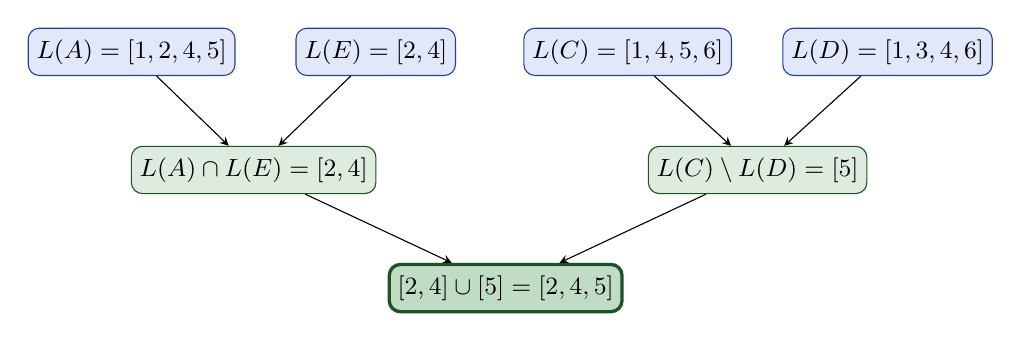
\begin{tikzpicture}[>=stealth,font=\small,
  list/.style={draw=PlotBlue!75!black,rounded corners,fill=PlotBlue!14,
    inner sep=3pt,minimum height=0.6cm},
  res/.style={draw=PlotGreen!60!black,rounded corners,fill=PlotGreen!16,
    inner sep=3pt,minimum height=0.6cm}]
  \node[list] (A) at (-4.9,0) {$L(A)=[1,2,4,5]$};
  \node[list] (E) at (-1.8,0) {$L(E)=[2,4]$};
  \node[list] (C) at (1.4,0) {$L(C)=[1,4,5,6]$};
  \node[list] (D) at (4.7,0) {$L(D)=[1,3,4,6]$};
  \node[res] (AE) at (-3.35,-1.5) {$L(A)\cap L(E)=[2,4]$};
  \node[res] (CD) at (3.05,-1.5) {$L(C)\setminus L(D)=[5]$};
  \node[res,very thick,fill=PlotGreen!30] (R) at (-0.15,-3)
    {$[2,4]\cup[5]=[2,4,5]$};
  \draw[->] (A) -- (AE);
  \draw[->] (E) -- (AE);
  \draw[->] (C) -- (CD);
  \draw[->] (D) -- (CD);
  \draw[->] (AE) -- (R);
  \draw[->] (CD) -- (R);
\end{tikzpicture}
\end{center}
\end{framedexample}

\Needspace{14\baselineskip}
\subsection{The same pointers, different rules}

All three operations scan the two sorted lists from left to right
with one pointer each, as in Algorithm~\ref{alg:posting-intersection}.
Only the action taken at each step changes:
\begin{center}
\small
\begin{tabular}{l|>{\raggedright\arraybackslash}p{3.2cm}%
  |>{\raggedright\arraybackslash}p{3.9cm}%
  |>{\raggedright\arraybackslash}p{3.6cm}}
  Query & Same identifier & Different identifiers & One list ends\\\hline
  $L$ AND $M$ & output it; advance both & advance the smaller & stop\\[2pt]
  $L$ OR $M$ & output it once; advance both & output the smaller; advance it
    & copy the rest of the other list\\[2pt]
  $L$ AND NOT $M$ & skip it; advance both & output the smaller only if it
    is in $L$; advance it & if $M$ ends, copy the rest of $L$; if $L$ ends,
    stop
\end{tabular}
\end{center}
Every pointer still moves only forwards, so each operation costs
$O(\abs L+\abs M)$. A query combining several operations therefore
costs $O\bigl(\sum_{t\in Q}n_t\bigr)$, as for AND.

\section{Faster ranked search}\label{sec:faster-ranked-search}

We return to ranked search (Section~\ref{sec:vector-search}): given a
query vector $\mathbf q$ and an integer $K$, return the $K$ documents
with the largest cosine similarity to $\mathbf q$. Scanning every
document costs $\Theta(Nm)$. Can we avoid looking at every document
and every term?

\subsection{Searching inside one cluster}

Offline, we can group the documents into \emph{clusters} of similar
documents and give each cluster a representative vector. Online, we
first find the cluster whose representative is closest to the query,
then compute cosine similarities only for the documents in that
cluster.

\Needspace{14\baselineskip}
\begin{center}
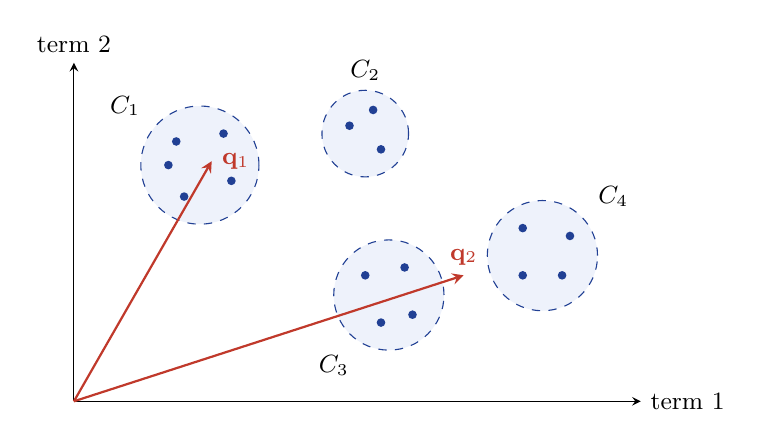
\begin{tikzpicture}[>=stealth,font=\small,
  doc/.style={circle,fill=PlotBlue!70!black,inner sep=1.1pt},
  cl/.style={draw=PlotBlue!70!black,dashed,fill=PlotBlue!8}]
  \draw[->] (0,0) -- (7.2,0) node[right] {term $1$};
  \draw[->] (0,0) -- (0,4.3) node[above] {term $2$};
  \filldraw[cl] (1.6,3.0) circle (0.75);
  \filldraw[cl] (3.7,3.4) circle (0.55);
  \filldraw[cl] (4.0,1.35) circle (0.7);
  \filldraw[cl] (5.95,1.85) circle (0.7);
  \node at (0.65,3.75) {$C_1$};
  \node at (3.7,4.2) {$C_2$};
  \node at (3.3,0.45) {$C_3$};
  \node at (6.85,2.6) {$C_4$};
  \foreach \p in {(1.3,3.3),(1.9,3.4),(1.4,2.6),(2.0,2.8),(1.2,3.0),
      (3.5,3.5),(3.9,3.2),(3.8,3.7),
      (3.7,1.6),(4.3,1.1),(3.9,1.0),(4.2,1.7),
      (5.7,2.2),(6.2,1.6),(6.3,2.1),(5.7,1.6)}
    \node[doc] at \p {};
  \draw[->,PlotRed,thick] (0,0) -- (1.75,3.05) node[right] {$\mathbf q_1$};
  \draw[->,PlotRed,thick] (0,0) -- (4.95,1.6) node[above] {$\mathbf q_2$};
\end{tikzpicture}
\end{center}
For $\mathbf q_1$, the closest documents are clearly in $C_1$. The query
$\mathbf q_2$ lies between $C_3$ and $C_4$, so its best documents may
belong to either cluster: searching only one of them can miss good
results. Clustering makes search faster, but the answer is only
approximate.

\subsection{Scoring only documents that share a query term}

Write $d_{i,t}$ for the weight of term $t$ in document $D_i$ and $q_t$
for its weight in the query. All weights are nonnegative, so the dot
product
\[
  \mathbf q\cdot\mathbf d_i=\sum_{t\in Q}q_t\,d_{i,t}
\]
is positive only if $D_i$ contains at least one query term. Every other
document has similarity $0$. The documents that can score are exactly
those in the posting lists of the query terms.

To compute the weights from the index, we extend each posting list:
each entry stores a pair $(i,\operatorname{TF}(t,D_i))$ instead of the
identifier alone. The cosine similarity then splits into a part
computed online and parts that do not depend on the documents or on
the query:
\[
  \operatorname{sim}_{\cos}(\mathbf q,\mathbf d_i)
  =\frac{\overbrace{\textstyle\sum_{t\in Q}q_t\,d_{i,t}}^{\text{online,
      from the posting lists}}}
    {\underbrace{\norm{\mathbf q}_2}_{\text{same for every }i}\,
     \underbrace{\norm{\mathbf d_i}_2}_{\text{stored offline}}}.
\]
\begin{itemize}
  \item $\norm{\mathbf q}_2$ is the same for every document, so it does
    not change the ranking and we can ignore it.
  \item $\norm{\mathbf d_i}_2$ does not depend on the query: we compute
    it offline and store it with the document.
  \item $\operatorname{IDF}(t)=\log(N/n_t)$ depends only on the length
    $n_t$ of the posting list $L(t)$, so it is also available offline.
\end{itemize}

\Needspace{22\baselineskip}
\begin{framedalgo}{Top-$K$ search with an inverted index}\label{alg:ranked-index}
\begin{algorithmic}[1]
  \Function{TopK}{$Q,K$}
    \State $S\gets$ an empty map from documents to scores
    \For{each term $t\in Q$}
      \For{each pair $(i,\mathit{tf})$ in $L(t)$}
        \State $S[i]\gets S[i]+q_t\cdot\mathit{tf}\cdot\operatorname{IDF}(t)$
          \Comment{missing entries start at $0$}
      \EndFor
    \EndFor
    \For{each document $i$ in $S$}
      \State $S[i]\gets S[i]/\norm{\mathbf d_i}_2$ \Comment{norm stored offline}
    \EndFor
    \State \Return the $K$ documents with the largest scores in $S$
  \EndFunction
\end{algorithmic}
\end{framedalgo}

The loops read each entry of the query's posting lists once, in
$O\bigl(\sum_{t\in Q}n_t\bigr)$ time. Only the $c\leq\sum_{t\in Q}n_t$
documents found in those lists receive a score, and sorting them
costs $O(c\log c)$. When the query terms are rare, this is far less
than the $\Theta(Nm+N\log N)$ needed to score and sort every document.

\Needspace{26\baselineskip}
\begin{framedexample}{Scoring the query $Q=\{C,E\}$}\label{ex:ranked-index}
For simplicity, give every term the same weight: $q_t=1$ for the query
terms and $d_{i,t}=\operatorname{TF}(t,D_i)$. Take the six documents of
Example~\ref{ex:inverted-index}, now with repeated terms:
\[
\begin{aligned}
  D_1&:A\,B\,C\,D, & D_2&:A\,B\,E\,G, & D_3&:B\,D\,F,\\
  D_4&:A\,C\,C\,D\,D\,E, & D_5&:A\,C\,G, & D_6&:C\,C\,C\,D\,G.
\end{aligned}
\]
The posting lists of the query terms store (document, TF) pairs:
\[
  L(C)=[(1,1),(4,2),(5,1),(6,3)],\qquad L(E)=[(2,1),(4,1)].
\]
Add up the TF values of each document found in these two lists, then
divide by its stored norm:
\begin{center}
\begin{tabular}{c|c|c|c}
  Document & $\operatorname{TF}(C)+\operatorname{TF}(E)$
    & $\norm{\mathbf d_i}_2$ (offline) & Score\\\hline
  $1$ & $1+0=1$ & $\sqrt4=2$ & $0.50$\\
  $2$ & $0+1=1$ & $\sqrt4=2$ & $0.50$\\
  $4$ & $2+1=3$ & $\sqrt{10}\approx3.16$ & $\mathbf{0.95}$\\
  $5$ & $1+0=1$ & $\sqrt3\approx1.73$ & $0.58$\\
  $6$ & $3+0=3$ & $\sqrt{11}\approx3.32$ & $\mathbf{0.90}$
\end{tabular}
\end{center}
For $K=2$ we return $D_4$ and $D_6$. Document $3$ is never examined,
because it contains neither $C$ nor $E$. Dividing every score by
$\norm{\mathbf q}_2=\sqrt2$ would give the exact cosines, with the same
ranking.
\end{framedexample}

With TF-IDF weights, the procedure is the same: multiply each TF by
$\operatorname{IDF}(t)$, computed from the list length $n_t$, and store
the norms of the TF-IDF vectors. In the example,
$\operatorname{IDF}(E)=\log(6/2)$ is larger than
$\operatorname{IDF}(C)=\log(6/4)$, so $E$ would count more than $C$.

\chapter{Sorting}

\lecturestart{26 October}

\section{The sorting problem}

\emph{Sorting} means arranging elements in order. We begin with a
simple goal: given a list of numbers, arrange them from smallest to
largest.

\begin{framedproblem}{Sorting}
\textbf{Input:} an array $A$ of numbers, not necessarily sorted.

\textbf{Output:} an array containing the same elements as $A$ in
nondecreasing order, preserving every occurrence of each value.
\end{framedproblem}

\begin{framedexample}{The same numbers, in a different order}
\begin{center}
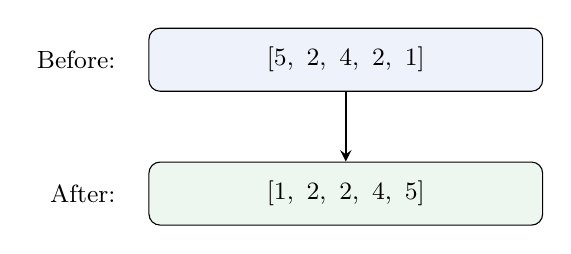
\begin{tikzpicture}[font=\small,>=stealth]
  \node[draw,rounded corners,fill=PlotBlue!8,
    minimum width=5cm,minimum height=0.8cm] (before) at (0,0)
    {$[5,\ 2,\ 4,\ 2,\ 1]$};
  \node[anchor=east] at (-2.8,0) {Before:};
  \node[draw,rounded corners,fill=PlotGreen!8,
    minimum width=5cm,minimum height=0.8cm] (after) at (0,-1.7)
    {$[1,\ 2,\ 2,\ 4,\ 5]$};
  \node[anchor=east] at (-2.8,-1.7) {After:};
  \draw[->,thick] (before.south) -- (after.north);
\end{tikzpicture}
\end{center}
The result must satisfy two conditions:
\begin{enumerate}
  \item Each number is less than or equal to the next one.
  \item The elements remain the same: only their order changes.
    In particular, both occurrences of $2$ must remain in the result.
\end{enumerate}
\end{framedexample}

With five numbers, we can easily do this by hand. A computer needs
precise instructions that also work for millions of elements. We
will study different algorithms for the same sorting problem,
examining how they work and how much time they require.

\section{MergeSort}

The first sorting algorithm we study is \emph{MergeSort}.
For example, we may start from
\[
  A=[2,10,7,16,3,8,9,1,11,13,14,20,17].
\]
\subsection{How Merge works: always take the smaller current element}

\Needspace{10\baselineskip}
Before studying the complete algorithm, we focus our attention on
the function \textsc{Merge}, a building block used by MergeSort.

\begin{framedproblem}{Merging two sorted arrays}
\textbf{Input:} two arrays $A_1$ and $A_2$, each already sorted in
nondecreasing order.

\textbf{Output:} one sorted array containing all the elements of both
arrays, preserving every occurrence of each value.
\end{framedproblem}

\begin{framedexample}{The input and output of Merge}
Consider the following separate example of a call to
$\textsc{Merge}(A_1,A_2)$:
\[
  A_1=[2,4,7,10,13],\qquad A_2=[1,3,5,6,8,9,16,17].
\]
We want one array containing all their values, in order:
\begin{center}
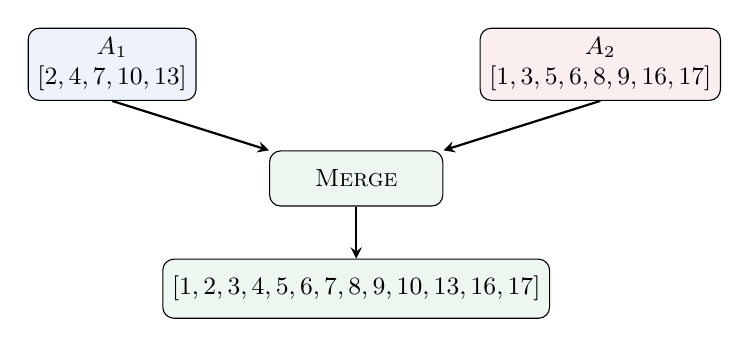
\begin{tikzpicture}[font=\small,>=stealth]
  \node[draw,rounded corners,fill=PlotBlue!8,align=center,
    minimum height=0.85cm] (left) at (-3.1,0)
    {$A_1$\\$[2,4,7,10,13]$};
  \node[draw,rounded corners,fill=PlotRed!8,align=center,
    minimum height=0.85cm] (right) at (3.1,0)
    {$A_2$\\$[1,3,5,6,8,9,16,17]$};
  \node[draw,rounded corners,fill=PlotGreen!8,
    minimum width=2.2cm,minimum height=0.7cm] (merge) at (0,-1.45)
    {\textsc{Merge}};
  \node[draw,rounded corners,fill=PlotGreen!8,
    minimum height=0.75cm] (result) at (0,-2.85)
    {$[1,2,3,4,5,6,7,8,9,10,13,16,17]$};
  \draw[->,thick] (left.south) -- (merge.north west);
  \draw[->,thick] (right.south) -- (merge.north east);
  \draw[->,thick] (merge.south) -- (result.north);
\end{tikzpicture}
\end{center}
The first array has $5$ elements and the second has $8$, so the
output must contain $5+8=13$ elements.
\end{framedexample}

Because both input arrays are sorted, the smallest element still
available in each array is its first unprocessed element. To choose
the next output value, we only need to compare those two elements.

Place a pointer $i$ at the start of $A_1$ and a pointer $j$ at the
start of $A_2$. Create an empty output array $B$. At each step:
\begin{enumerate}
  \item Compare $A_1[i]$ and $A_2[j]$.
  \item Append the smaller value to $B$.
  \item Advance only the pointer of the array from which we took it.
\end{enumerate}
If the two values are equal, take the one from $A_1$ first. The other
occurrence remains available in $A_2$, so neither occurrence is lost.

\begin{framedexample}{Following Merge on the two arrays}\label{ex:merge-steps}
Start with
\[
  A_1=[2,4,7,10,13],\qquad A_2=[1,3,5,6,8,9,16,17],\qquad B=[\,].
\]
\textbf{Step 1: compare $2$ and $1$.}
\[
  A_1=[\boxed{2},4,7,10,13],\qquad
  A_2=[\boxed{1},3,5,6,8,9,16,17].
\]
Take $1$ from $A_2$: $B=[1]$. Advance its pointer to $3$; the
pointer in $A_1$ stays at $2$.

\textbf{Step 2: compare $2$ and $3$.}
\[
  A_1=[\boxed{2},4,7,10,13],\qquad
  A_2=[1,\boxed{3},5,6,8,9,16,17].
\]
Take $2$ from $A_1$: $B=[1,2]$. Advance its pointer to $4$.

\textbf{Step 3: compare $4$ and $3$.}
\[
  A_1=[2,\boxed{4},7,10,13],\qquad
  A_2=[1,\boxed{3},5,6,8,9,16,17].
\]
Take $3$ from $A_2$: $B=[1,2,3]$. Advance its pointer to $5$.

\textbf{Continue with the same rule.}
The following rows show the current values before each remaining
comparison and the output after taking the smaller one:
\begin{center}
\small
\begin{tabular}{rr|c|l}
  $A_1[i]$ & $A_2[j]$ & Take & Output $B$\\\hline
  $4$ & $5$ & $4$ & $[1,2,3,4]$\\
  $7$ & $5$ & $5$ & $[1,2,3,4,5]$\\
  $7$ & $6$ & $6$ & $[1,2,3,4,5,6]$\\
  $7$ & $8$ & $7$ & $[1,2,3,4,5,6,7]$\\
  $10$ & $8$ & $8$ & $[1,2,3,4,5,6,7,8]$\\
  $10$ & $9$ & $9$ & $[1,2,3,4,5,6,7,8,9]$\\
  $10$ & $16$ & $10$ & $[1,2,3,4,5,6,7,8,9,10]$\\
  $13$ & $16$ & $13$ & $[1,2,3,4,5,6,7,8,9,10,13]$
\end{tabular}
\end{center}
\textbf{When one input is exhausted, copy the rest of the other.}
After taking $13$, $A_1$ is exhausted. The remaining values in $A_2$
are $16,17$. They are already sorted and can be appended directly:
\[
  B=[1,2,3,4,5,6,7,8,9,10,13,16,17].
\]
\end{framedexample}

The algorithm below uses indices starting at $1$. The output array
$B$ has space for $\abs{A_1}+\abs{A_2}$ elements, and $k$ indicates
the next output position to fill.

\Needspace{30\baselineskip}
\begin{framedalgo}{Merge two sorted arrays}\label{alg:merge}
\begin{algorithmic}[1]
  \Function{Merge}{$A_1,A_2$}
    \State $n_1\gets\abs{A_1}$, $n_2\gets\abs{A_2}$
    \State Allocate an array $B$ of length $n_1+n_2$
    \State $i\gets1$, $j\gets1$, $k\gets1$
    \While{$i\leq n_1$ and $j\leq n_2$}
      \If{$A_1[i]\leq A_2[j]$}
        \State $B[k]\gets A_1[i]$
        \State $i\gets i+1$
      \Else
        \State $B[k]\gets A_2[j]$
        \State $j\gets j+1$
      \EndIf
      \State $k\gets k+1$
    \EndWhile
    \While{$i\leq n_1$}
      \State $B[k]\gets A_1[i]$
      \State $i\gets i+1$, $k\gets k+1$
    \EndWhile
    \While{$j\leq n_2$}
      \State $B[k]\gets A_2[j]$
      \State $j\gets j+1$, $k\gets k+1$
    \EndWhile
    \State \Return $B$
  \EndFunction
\end{algorithmic}
\end{framedalgo}

\subsection{Why the result is sorted, and how much Merge costs}

At every step, the next value must be the smaller of the two current
elements: all later elements of each input are at least as large as
that input's current element. Appending the smaller one therefore
keeps $B$ sorted.

\Needspace{17\baselineskip}
Let $n_1=\abs{A_1}$ be the number of elements in the first array and
$n_2=\abs{A_2}$ the number of elements in the second. Merge copies
each of these elements into $B$ exactly once: $n_1$ copies come from
$A_1$ and $n_2$ from $A_2$, for a total of $n_1+n_2$ copies.
The pointers only move forwards, and each copy and pointer update
takes constant time. Its running time is therefore
\[
  \boxed{T_{\mathrm{Merge}}(n_1,n_2)=\Theta(n_1+n_2).}
\]
The separate output array uses $\Theta(n_1+n_2)$ additional space;
the three indices require only constant extra space.

\section{MergeSort: split, sort the halves, and merge}

Merge combines two arrays that are already sorted. To sort an arbitrary
array $A$, we first split it into two halves and sort each half using
MergeSort itself. We then pass the two sorted results to Merge.

\textbf{When can we stop splitting?} An array with zero or one element
is already sorted, so we return it immediately. This is the base case.

For $n>1$, let $m=\lceil n/2\rceil$. Using indices starting at $1$,
the two halves are
\[
  A_1=A[1,\ldots,m],\qquad A_2=A[m+1,\ldots,n].
\]
The first half contains $m$ elements and the second contains $n-m$.
For our $13$-element input, $m=7$: the halves contain positions
$1$ through $7$ and positions $8$ through $13$.

\Needspace{20\baselineskip}
\begin{framedalgo}{MergeSort}\label{alg:mergesort}
\begin{algorithmic}[1]
  \Function{MergeSort}{$A$}
    \State $n\gets\abs{A}$ \Comment{$\Theta(1)$}
    \If{$n\leq1$} \Comment{$\Theta(1)$}
      \State \Return $A$ \Comment{$\Theta(1)$}
    \EndIf
    \State $m\gets\lceil n/2\rceil$ \Comment{$\Theta(1)$}
    \State $A_1\gets A[1,\ldots,m]$ \Comment{$\Theta(m)$ to copy}
    \State $A_2\gets A[m+1,\ldots,n]$ \Comment{$\Theta(n-m)$ to copy}
    \State $A_1\gets\Call{MergeSort}{A_1}$ \Comment{$T(m)$}
    \State $A_2\gets\Call{MergeSort}{A_2}$ \Comment{$T(n-m)$}
    \State \Return $\Call{Merge}{A_1,A_2}$ \Comment{$\Theta(n)$}
  \EndFunction
\end{algorithmic}
\end{framedalgo}

\Needspace{34\baselineskip}
\begin{framedexample}{MergeSort on the 13-element array}\label{ex:mergesort-thirteen}
MergeSort on $A=[2,10,7,16,3,8,9,1,11,13,14,20,17]$. Blue arrays
are still unsorted; green arrays are sorted.
\begin{center}
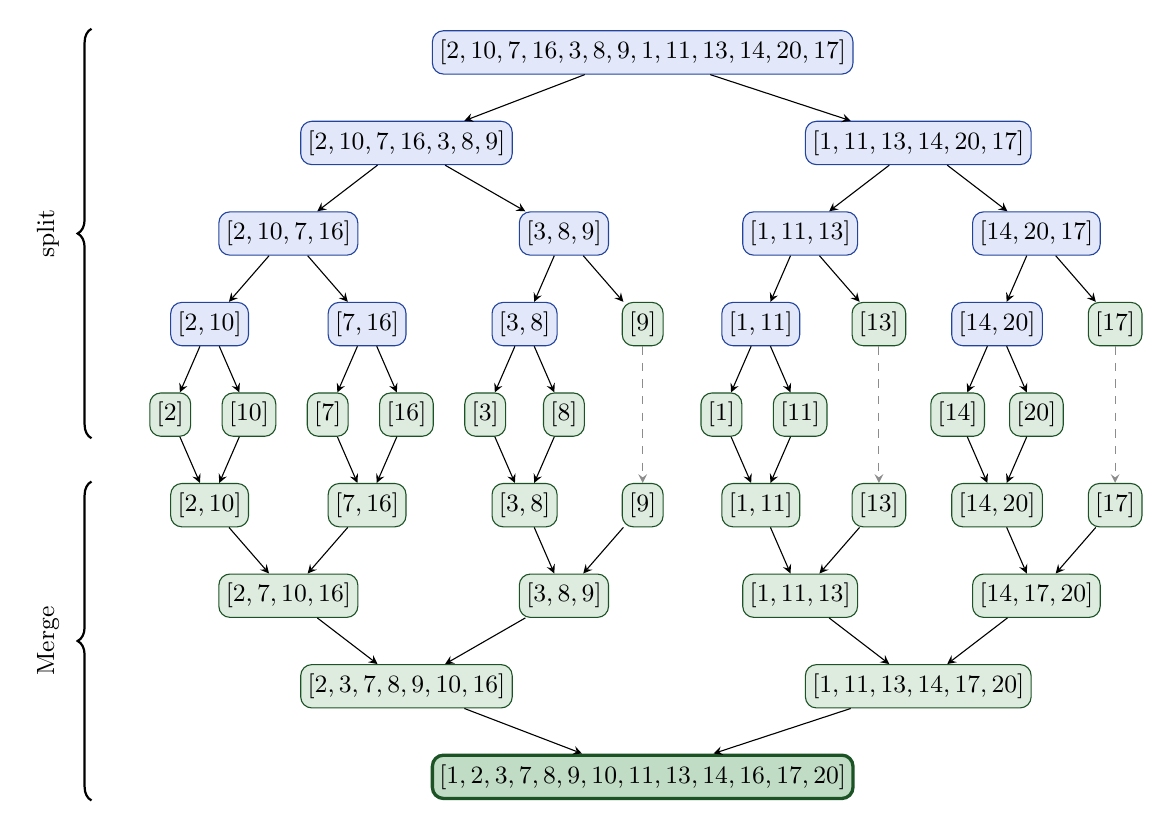
\begin{tikzpicture}[>=stealth,font=\small,
  arr/.style={draw=PlotBlue!75!black,rounded corners,
    minimum height=0.55cm,inner sep=2.5pt,fill=PlotBlue!14},
  sorted/.style={arr,draw=PlotGreen!60!black,fill=PlotGreen!16},
  pass/.style={->,dashed,draw=black!45}]
  % Split: each array is divided at position ceil(n/2).
  \node[arr] (s0) at (0,0) {$[2,10,7,16,3,8,9,1,11,13,14,20,17]$};
  \node[arr] (s1a) at (-3,-1.15) {$[2,10,7,16,3,8,9]$};
  \node[arr] (s1b) at (3.5,-1.15) {$[1,11,13,14,20,17]$};
  \node[arr] (s2a) at (-4.5,-2.3) {$[2,10,7,16]$};
  \node[arr] (s2b) at (-1,-2.3) {$[3,8,9]$};
  \node[arr] (s2c) at (2,-2.3) {$[1,11,13]$};
  \node[arr] (s2d) at (5,-2.3) {$[14,20,17]$};
  \node[arr] (s3a) at (-5.5,-3.45) {$[2,10]$};
  \node[arr] (s3b) at (-3.5,-3.45) {$[7,16]$};
  \node[arr] (s3c) at (-1.5,-3.45) {$[3,8]$};
  \node[sorted] (s3d) at (0,-3.45) {$[9]$};
  \node[arr] (s3e) at (1.5,-3.45) {$[1,11]$};
  \node[sorted] (s3f) at (3,-3.45) {$[13]$};
  \node[arr] (s3g) at (4.5,-3.45) {$[14,20]$};
  \node[sorted] (s3h) at (6,-3.45) {$[17]$};
  \foreach \x/\v in {-6/2,-5/10,-4/7,-3/16,-2/3,-1/8,1/1,2/11,4/14,5/20}
    \node[sorted] (b\v) at (\x,-4.6) {$[\v]$};
  % Merge: pairs of sorted arrays are combined.
  \node[sorted] (m3a) at (-5.5,-5.75) {$[2,10]$};
  \node[sorted] (m3b) at (-3.5,-5.75) {$[7,16]$};
  \node[sorted] (m3c) at (-1.5,-5.75) {$[3,8]$};
  \node[sorted] (m3d) at (0,-5.75) {$[9]$};
  \node[sorted] (m3e) at (1.5,-5.75) {$[1,11]$};
  \node[sorted] (m3f) at (3,-5.75) {$[13]$};
  \node[sorted] (m3g) at (4.5,-5.75) {$[14,20]$};
  \node[sorted] (m3h) at (6,-5.75) {$[17]$};
  \node[sorted] (m2a) at (-4.5,-6.9) {$[2,7,10,16]$};
  \node[sorted] (m2b) at (-1,-6.9) {$[3,8,9]$};
  \node[sorted] (m2c) at (2,-6.9) {$[1,11,13]$};
  \node[sorted] (m2d) at (5,-6.9) {$[14,17,20]$};
  \node[sorted] (m1a) at (-3,-8.05) {$[2,3,7,8,9,10,16]$};
  \node[sorted] (m1b) at (3.5,-8.05) {$[1,11,13,14,17,20]$};
  \node[sorted,very thick,fill=PlotGreen!30]
    (m0) at (0,-9.2) {$[1,2,3,7,8,9,10,11,13,14,16,17,20]$};
  % Split arrows.
  \foreach \p/\c in {s0/s1a,s0/s1b,s1a/s2a,s1a/s2b,s1b/s2c,s1b/s2d,
      s2a/s3a,s2a/s3b,s2b/s3c,s2b/s3d,s2c/s3e,s2c/s3f,s2d/s3g,s2d/s3h,
      s3a/b2,s3a/b10,s3b/b7,s3b/b16,s3c/b3,s3c/b8,s3e/b1,s3e/b11,
      s3g/b14,s3g/b20}
    \draw[->] (\p) -- (\c);
  % One-element arrays are already sorted and are returned unchanged.
  \foreach \a/\b in {s3d/m3d,s3f/m3f,s3h/m3h}
    \draw[pass] (\a) -- (\b);
  % Merge arrows.
  \foreach \c/\p in {b2/m3a,b10/m3a,b7/m3b,b16/m3b,b3/m3c,b8/m3c,
      b1/m3e,b11/m3e,b14/m3g,b20/m3g,
      m3a/m2a,m3b/m2a,m3c/m2b,m3d/m2b,m3e/m2c,m3f/m2c,m3g/m2d,m3h/m2d,
      m2a/m1a,m2b/m1a,m2c/m1b,m2d/m1b,m1a/m0,m1b/m0}
    \draw[->] (\c) -- (\p);
  \draw[decorate,decoration={brace,amplitude=5pt},thick]
    (-7,-4.9) -- (-7,0.3)
    node[midway,left=8pt,rotate=90,anchor=south] {split};
  \draw[decorate,decoration={brace,amplitude=5pt},thick]
    (-7,-9.5) -- (-7,-5.45)
    node[midway,left=8pt,rotate=90,anchor=south] {Merge};
\end{tikzpicture}
\end{center}
\end{framedexample}

\subsection{Running time: expanding the recurrence}

Let $T(n)$ be the number of steps for an array of $n$ elements.
Assume first that $n$ is a power of $2$, so $m=n-m=n/2$.
Counting the steps of Algorithm~\ref{alg:mergesort} gives a
\emph{recurrence}:
\[
  T(n)=
  \begin{cases}
    c_1, & n\leq1,\\
    2T(n/2)+c_2n+c_3, & n>1,
  \end{cases}
\]
Here $c_1$ is the base-case cost, $c_2n$ accounts for copying the
halves and merging, and $c_3$ is the remaining constant work.
The constants are positive and independent of $n$.

We solve this recurrence by repeatedly substituting it into itself.
As in the earlier recurrence expansions, a term and its replacement
are underlined in the same colour.

\Needspace{17\baselineskip}
\textbf{First expansion.}
Apply the recurrence to an input of size $n/2$:
\[
  T(n/2)=2T(n/4)+c_2\frac n2+c_3.
\]
Substitute this expression for $T(n/2)$ and distribute the outer $2$:
\begin{align*}
  T(n)&=2\,\cul{PlotRed}{T(n/2)}+c_2n+c_3\\
      &=2\,\cul{PlotRed}{\left[2T(n/4)+c_2\frac n2+c_3\right]}
        +c_2n+c_3\\
      &=4T(n/4)+c_2n+2c_3+c_2n+c_3\\
      &=4T(n/4)+2c_2n+3c_3.
\end{align*}
There are now four subproblems of size $n/4$. The two linear
contributions add up to $2c_2n$, and the constant contributions
add up to $3c_3$.

\Needspace{13\baselineskip}
\textbf{Second expansion.}
Now replace $T(n/4)$ using the same recurrence:
\begin{align*}
  T(n)&=4\,\cul{PlotBlue}{T(n/4)}+2c_2n+3c_3\\
      &=4\,\cul{PlotBlue}{\left[2T(n/8)+c_2\frac n4+c_3\right]}
        +2c_2n+3c_3\\
      &=8T(n/8)+c_2n+4c_3+2c_2n+3c_3\\
      &=8T(n/8)+3c_2n+7c_3.
\end{align*}

\Needspace{12\baselineskip}
\textbf{Third expansion.}
\begin{align*}
  T(n)&=8\,\cul{PlotGreen}{T(n/8)}+3c_2n+7c_3\\
      &=8\,\cul{PlotGreen}{\left[2T(n/16)+c_2\frac n8+c_3\right]}
        +3c_2n+7c_3\\
      &=16T(n/16)+4c_2n+15c_3.
\end{align*}

\textbf{The general pattern.}
Each substitution doubles the number of subproblems and halves
their size. At each level, the linear work adds up to $c_2n$:
\[
  1\cdot c_2n
  =2\cdot c_2\frac n2
  =4\cdot c_2\frac n4
  =\cdots=c_2n.
\]
After expanding $i$ levels, we therefore have
\[
  \boxed{T(n)=2^iT\!\left(\frac{n}{2^i}\right)
    +i\,c_2n+(2^i-1)c_3.}
\]
Here $2^iT(n/2^i)$ is the work still to be expanded, $i\,c_2n$
accounts for the $i$ levels already expanded, and the constant work
comes from $1+2+4+\cdots+2^{i-1}=2^i-1$ calls at those levels.

\Needspace{20\baselineskip}
\textbf{When do we stop?}
We reach the base case when each remaining subproblem has size $1$:
\[
  \frac{n}{2^i}=1
  \quad\Longrightarrow\quad 2^i=n
  \quad\Longrightarrow\quad i=\log_2 n.
\]
Substituting $i=\log_2 n$ and $T(1)=c_1$ gives
\begin{align*}
  T(n)&=nT(1)+c_2n\log_2 n+(n-1)c_3\\
      &=c_1n+c_2n\log_2 n+c_3(n-1).
\end{align*}
The first and last terms are linear in $n$. The dominant term is
$c_2n\log_2 n$, so
\[
  \boxed{T(n)=\Theta(n\log n).}
\]
For a general $n$, the two recursive sizes are $\lceil n/2\rceil$
and $\lfloor n/2\rfloor$. The number of levels is
$\lceil\log_2 n\rceil$, and the same asymptotic bound holds.

\Needspace{29\baselineskip}
\textbf{Visualizing the work at each level.}
Each box below represents a recursive call and shows the number of
elements it sorts. The subarrays at each merging level therefore
contain $n$ elements altogether.

\begin{center}
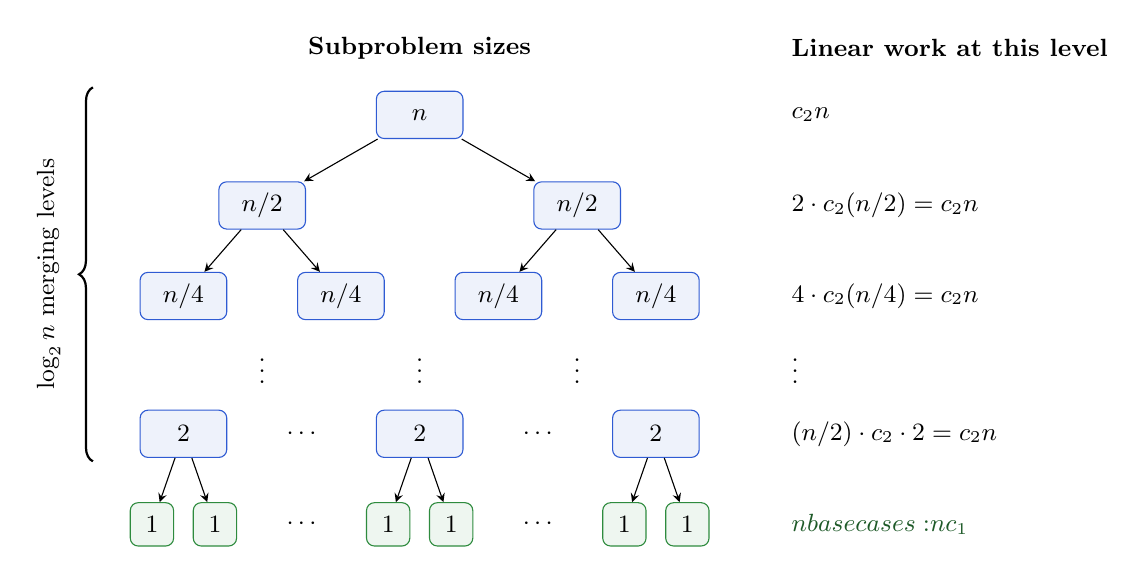
\begin{tikzpicture}[>=stealth,font=\small,
  call/.style={draw=PlotBlue,rounded corners=1mm,
    fill=PlotBlue!8,minimum width=1.1cm,minimum height=0.6cm},
  base/.style={draw=PlotGreen,rounded corners=1mm,
    fill=PlotGreen!8,minimum width=0.55cm,minimum height=0.55cm}]
  \node[font=\small\bfseries] at (4,0.85) {Subproblem sizes};
  \node[anchor=west,font=\small\bfseries] at (8.6,0.85)
    {Linear work at this level};
  \node[call] (root) at (4,0) {$n$};
  \node[call] (l) at (2,-1.15) {$n/2$};
  \node[call] (r) at (6,-1.15) {$n/2$};
  \node[call] (ll) at (1,-2.3) {$n/4$};
  \node[call] (lr) at (3,-2.3) {$n/4$};
  \node[call] (rl) at (5,-2.3) {$n/4$};
  \node[call] (rr) at (7,-2.3) {$n/4$};
  \draw[->] (root) -- (l);
  \draw[->] (root) -- (r);
  \draw[->] (l) -- (ll);
  \draw[->] (l) -- (lr);
  \draw[->] (r) -- (rl);
  \draw[->] (r) -- (rr);
  \node at (2,-3.15) {$\vdots$};
  \node at (4,-3.15) {$\vdots$};
  \node at (6,-3.15) {$\vdots$};
  \node[call] (p1) at (1,-4.05) {$2$};
  \node[call] (p2) at (4,-4.05) {$2$};
  \node[call] (p3) at (7,-4.05) {$2$};
  \node at (2.5,-4.05) {$\cdots$};
  \node at (5.5,-4.05) {$\cdots$};
  \foreach \x/\name in {0.6/b1,1.4/b2,3.6/b3,4.4/b4,6.6/b5,7.4/b6}
    \node[base] (\name) at (\x,-5.2) {$1$};
  \draw[->] (p1) -- (b1);
  \draw[->] (p1) -- (b2);
  \draw[->] (p2) -- (b3);
  \draw[->] (p2) -- (b4);
  \draw[->] (p3) -- (b5);
  \draw[->] (p3) -- (b6);
  \node at (2.5,-5.2) {$\cdots$};
  \node at (5.5,-5.2) {$\cdots$};
  \node[anchor=west] at (8.6,0) {$c_2n$};
  \node[anchor=west] at (8.6,-1.15) {$2\cdot c_2(n/2)=c_2n$};
  \node[anchor=west] at (8.6,-2.3) {$4\cdot c_2(n/4)=c_2n$};
  \node[anchor=west] at (8.6,-3.15) {$\vdots$};
  \node[anchor=west] at (8.6,-4.05) {$(n/2)\cdot c_2\cdot2=c_2n$};
  \node[anchor=west,text=PlotGreen!65!black] at (8.6,-5.2)
    {$n\text{ base cases: }nc_1$};
  \draw[decorate,decoration={brace,amplitude=5pt},thick]
    (-0.15,-4.4) -- (-0.15,0.35)
    node[midway,left=8pt,rotate=90,anchor=south]
      {$\log_2 n$ merging levels};
\end{tikzpicture}
\end{center}
Each merging level contributes $c_2n$ linear work. There are
$\log_2 n$ such levels, giving $c_2n\log_2 n$ altogether.
At the bottom, the $n$ single-element inputs contribute $nc_1$.

\chapter{Randomized Algorithms}

\section{Making random choices inside an algorithm}

A deterministic algorithm follows the same execution whenever it
receives the same input. We now allow the algorithm to make random
choices during its execution. For example, a sorting algorithm may
choose a different element to work with first on each run.

\begin{frameddefn}{Randomized algorithm}\label{def:randomized-algorithm}
A \emph{randomized algorithm} uses random choices as part of its
computation. Even for a fixed input, different choices may lead to
different executions and running times.
\end{frameddefn}

For randomized QuickSort, every execution will still return a sorted
array. What changes with the random choices is the amount of work
needed to obtain it. To describe this cost, we first need to understand
an average taken over random outcomes.

\section{Expected value: averaging over random outcomes}

Imagine rolling a fair die many times and averaging the results.
Each of the six faces appears with probability $1/6$, so each face
contributes equally to the average.

\begin{frameddefn}{Random variable and expected value}\label{def:expected-value}
A discrete \emph{random variable} $X$ assigns a numerical value to
each random outcome. Its \emph{expected value} is the weighted average
of its possible values:
\[
  \E[X]=\sum_{x\in\operatorname{range}(X)}x\,\Prob(X=x).
\]
Each value $x$ is weighted by its probability of occurring.
\end{frameddefn}

\begin{framedexample}{One die, then two dice}\label{ex:dice-expectation}
\textbf{Step 1: one fair die.}
Let $Y$ be the number on its upper face. The possible values are
$1,2,3,4,5,6$, each with probability $1/6$. Thus
\begin{align*}
  \E[Y]&=1\cdot\frac16+2\cdot\frac16+3\cdot\frac16
    +4\cdot\frac16+5\cdot\frac16+6\cdot\frac16\\
    &=\frac{1+2+3+4+5+6}{6}=\frac{21}{6}=3.5.
\end{align*}
\textbf{Step 2: the sum of two fair independent dice.}
Let $X=Y_1+Y_2$. There are $6\cdot6=36$ equally likely ordered pairs
of faces. The table shows the sum for each pair:
\begin{center}
\begin{tabular}{c|rrrrrr}
  $Y_1\backslash Y_2$ & $1$ & $2$ & $3$ & $4$ & $5$ & $6$\\\hline
  $1$ & $2$ & $3$ & $4$ & $5$ & $6$ & $7$\\
  $2$ & $3$ & $4$ & $5$ & $6$ & $7$ & $8$\\
  $3$ & $4$ & $5$ & $6$ & $7$ & $8$ & $9$\\
  $4$ & $5$ & $6$ & $7$ & $8$ & $9$ & $10$\\
  $5$ & $6$ & $7$ & $8$ & $9$ & $10$ & $11$\\
  $6$ & $7$ & $8$ & $9$ & $10$ & $11$ & $12$
\end{tabular}
\end{center}
The sum $2$ occurs only for $(1,1)$, whereas $3$ occurs for $(1,2)$
and $(2,1)$. The sum $7$ occurs for six different pairs. Therefore
\[
  \Prob(X=2)=\frac1{36},\qquad
  \Prob(X=3)=\frac2{36},\qquad
  \Prob(X=7)=\frac6{36}.
\]
The possible sums are not equally likely. We can compute their
weighted average using the definition. A shorter calculation uses
\emph{linearity of expectation}: the expected value of a sum is the
sum of the expected values. Hence
\[
  \E[X]=\E[Y_1+Y_2]=\E[Y_1]+\E[Y_2]=3.5+3.5=7.
\]
\end{framedexample}

For a randomized algorithm, the running time on a fixed input is
also a random variable. Its expected running time averages over the
algorithm's random choices.

\section{QuickSort: choose a pivot and partition}

QuickSort sorts an array by choosing one of its elements as a
\emph{pivot}. It compares the remaining elements with that pivot and
separates them into two smaller arrays.

\Needspace{12\baselineskip}
\begin{frameddefn}{Pivot and partition}\label{def:quicksort-pivot}
Choose an index $p$ uniformly from $\{1,\ldots,n\}$ and let $v=A[p]$
be the pivot value. Excluding $A[p]$, form
\[
  A_1=[\text{elements of }A\text{ that are }\leq v],\qquad
  A_2=[\text{elements of }A\text{ that are }>v].
\]
Every remaining element goes into exactly one of these two arrays.
This separation is called \emph{partitioning}.
\end{frameddefn}

Now sort $A_1$ and $A_2$ recursively. If their sorted results are
$A'_1$ and $A'_2$, the answer is their concatenation with the pivot
between them:
\[
  [\,A'_1,\ v,\ A'_2\,].
\]
Every value in $A'_1$ is at most $v$, and every value in $A'_2$ is
greater than $v$. Once the two parts are sorted, placing them in this
order produces a sorted array. As before, an array with zero or one
element is already sorted and is returned immediately.

\subsection{The QuickSort algorithm}

Indices start at $1$. Appending to the temporary arrays is assumed
to take amortized constant time. The final concatenation copies the
two sorted parts and the pivot into the returned array.

\Needspace{23\baselineskip}
\begin{framedalgo}{Randomized QuickSort}\label{alg:randomized-quicksort}
\begin{algorithmic}[1]
  \Function{QuickSort}{$A$}
    \State $n\gets\abs{A}$ \Comment{$\Theta(1)$}
    \If{$n\leq1$}
      \State \Return $A$
    \EndIf
    \State Choose $p$ uniformly from $\{1,\ldots,n\}$
    \State $v\gets A[p]$
    \State $A_1\gets[\,]$, $A_2\gets[\,]$
    \For{$i=1,\ldots,n$} \Comment{$\Theta(n)$ in total}
      \If{$i\neq p$}
        \If{$A[i]\leq v$}
          \State Append $A[i]$ to $A_1$
        \Else
          \State Append $A[i]$ to $A_2$
        \EndIf
      \EndIf
    \EndFor
    \State $A'_1\gets\Call{QuickSort}{A_1}$ \Comment{$T(\abs{A_1})$}
    \State $A'_2\gets\Call{QuickSort}{A_2}$ \Comment{$T(\abs{A_2})$}
    \State \Return $\Call{Concatenate}{A'_1,[v],A'_2}$ \Comment{$\Theta(n)$}
  \EndFunction
\end{algorithmic}
\end{framedalgo}

The test $i\neq p$ excludes the selected pivot from both recursive
inputs. Other occurrences of the same value are kept in $A_1$.
Each recursive input has fewer than $n$ elements, so the algorithm
eventually reaches its base cases.

\subsection{Following the recursive calls}

We now run QuickSort on the 13-element array that MergeSort sorted in
Example~\ref{ex:mergesort-thirteen}.

\Needspace{22\baselineskip}
\begin{framedexample}{QuickSort on the 13-element array}\label{ex:quicksort-trace}
Each row is one level of recursive calls, and the circled values are
the random pivots. Once a pivot or a one-element array is placed, it
never moves again: the dashed arrows carry it to the sorted result.
\begin{center}
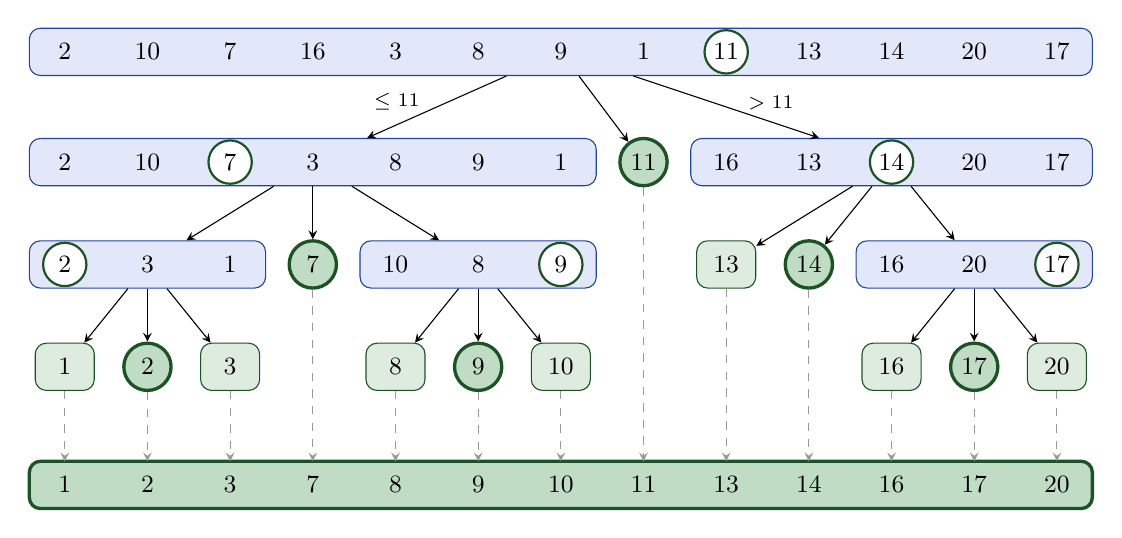
\begin{tikzpicture}[>=stealth,font=\small,x=1.05cm,y=1cm,
  sub/.style={draw=PlotBlue!75!black,rounded corners,fill=PlotBlue!14,
    minimum height=0.6cm,inner sep=0pt},
  done/.style={draw=PlotGreen!60!black,rounded corners,
    fill=PlotGreen!16,minimum height=0.6cm,minimum width=0.75cm,
    inner sep=0pt},
  final/.style={done,very thick,fill=PlotGreen!30},
  chosen/.style={circle,draw=PlotGreen!60!black,thick,fill=white,
    inner sep=0pt,minimum size=0.55cm},
  piv/.style={circle,draw=PlotGreen!60!black,very thick,
    fill=PlotGreen!30,inner sep=0pt,minimum size=0.6cm},
  drop/.style={->,dashed,draw=black!40}]
  % An array drawn over columns #4..#5 (style #1, name #2, height #3).
  % Column c is the final position of the c-th smallest value.
  \newcommand{\qsarr}[6][sub]{%
    \node[#1,minimum width={(#5-#4+1)*1.05cm-0.15cm}]
      (#2) at ({(#4+#5)/2},#3) {};
    \foreach \v [count=\c from #4] in {#6} \node at (\c,#3) {$\v$};}
  % Level 0: pivot 11.
  \qsarr{r0}{0}{1}{13}{2,10,7,16,3,8,9,1,11,13,14,20,17}
  \node[chosen] at (9,0) {$11$};
  % Level 1: pivots 7 and 14.
  \qsarr{a}{-1.4}{1}{7}{2,10,7,3,8,9,1}
  \node[chosen] at (3,-1.4) {$7$};
  \node[piv] (p11) at (8,-1.4) {$11$};
  \qsarr{b}{-1.4}{9}{13}{16,13,14,20,17}
  \node[chosen] at (11,-1.4) {$14$};
  % Level 2: pivots 2, 9 and 17.
  \qsarr{aa}{-2.7}{1}{3}{2,3,1}
  \node[chosen] at (1,-2.7) {$2$};
  \node[piv] (p7) at (4,-2.7) {$7$};
  \qsarr{ab}{-2.7}{5}{7}{10,8,9}
  \node[chosen] at (7,-2.7) {$9$};
  \node[done] (d13) at (9,-2.7) {$13$};
  \node[piv] (p14) at (10,-2.7) {$14$};
  \qsarr{bb}{-2.7}{11}{13}{16,20,17}
  \node[chosen] at (13,-2.7) {$17$};
  % Level 3: only pivots and one-element arrays remain.
  \node[done] (d1) at (1,-4) {$1$};
  \node[piv] (p2) at (2,-4) {$2$};
  \node[done] (d3) at (3,-4) {$3$};
  \node[done] (d8) at (5,-4) {$8$};
  \node[piv] (p9) at (6,-4) {$9$};
  \node[done] (d10) at (7,-4) {$10$};
  \node[done] (d16) at (11,-4) {$16$};
  \node[piv] (p17) at (12,-4) {$17$};
  \node[done] (d20) at (13,-4) {$20$};
  % Sorted result.
  \qsarr[final]{f}{-5.5}{1}{13}{1,2,3,7,8,9,10,11,13,14,16,17,20}
  \draw[->] (r0) -- (a)
    node[pos=0.6,above left,inner sep=1pt,font=\scriptsize] {$\leq11$};
  \draw[->] (r0) -- (b)
    node[pos=0.6,above right,inner sep=1pt,font=\scriptsize] {$>11$};
  \foreach \p/\c in {r0/p11,a/aa,a/p7,a/ab,b/d13,b/p14,b/bb,
      aa/d1,aa/p2,aa/d3,ab/d8,ab/p9,ab/d10,bb/d16,bb/p17,bb/d20}
    \draw[->] (\p) -- (\c);
  \foreach \n/\c in {p11/8,p7/4,d13/9,p14/10,d1/1,p2/2,d3/3,d8/5,
      p9/6,d10/7,d16/11,p17/12,d20/13}
    \draw[drop] (\n.south) -- (\c,-5.2);
\end{tikzpicture}
\end{center}
\end{framedexample}

\section{The cost of QuickSort}

For the running-time analysis in this section, assume that the $n$
values are distinct. Partitioning compares the pivot with the other
$n-1$ elements. If $k$ values are smaller than the pivot, the two
recursive sizes are $k$ and $n-1-k$. A call therefore has the form
\[
  T(n)=T(k)+T(n-1-k)+\Theta(n).
\]
The linear term includes partitioning and the final concatenation.
The random pivot determines $k$, so it determines how balanced the
two recursive inputs will be.

\subsection{Balanced partitions and the worst case}

\textbf{Balanced partitions.}
A pivot near the middle of the sorted order leaves two inputs of
roughly half the size. Repeated balanced partitions give logarithmic
depth, with at most linear work across each level. This leads to
$\Theta(n\log n)$ time.

\Needspace{10\baselineskip}
\textbf{The worst case.}
If the pivot is always an extreme value (the smallest or the largest),
one recursive input is empty and the other has $n-1$ elements. The
next nonempty call has size $n-1$, then $n-2$, and so on. The number
of pivot comparisons is
\[
  (n-1)+(n-2)+\cdots+1=\frac{n(n-1)}2=\Theta(n^2).
\]

\Needspace{25\baselineskip}
\begin{center}
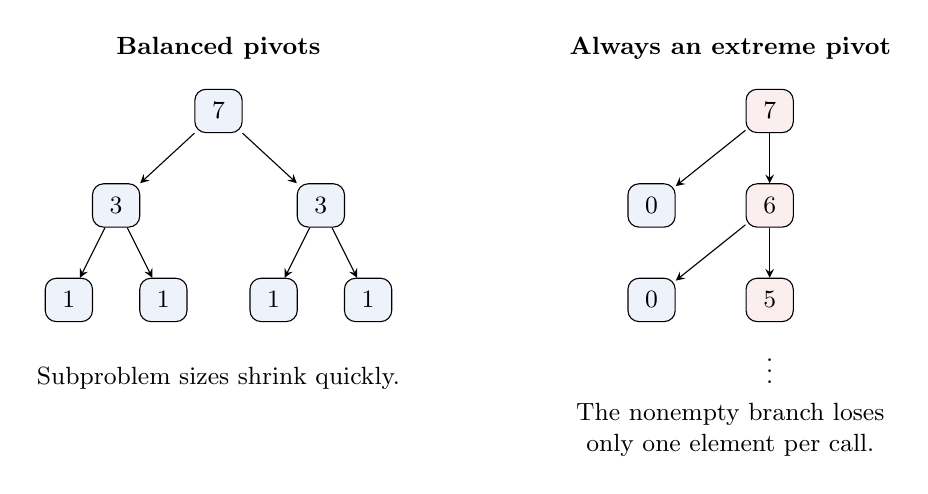
\begin{tikzpicture}[>=stealth,font=\small,
  size/.style={draw,rounded corners,minimum width=0.6cm,
    minimum height=0.55cm,fill=PlotBlue!8}]
  \node[font=\small\bfseries] at (-3,0.6) {Balanced pivots};
  \node[font=\small\bfseries] at (3.5,0.6) {Always an extreme pivot};
  \node[size] (a) at (-3,-0.2) {$7$};
  \node[size] (l) at (-4.3,-1.4) {$3$};
  \node[size] (r) at (-1.7,-1.4) {$3$};
  \foreach \x/\name in {-4.9/a1,-3.7/a2,-2.3/a3,-1.1/a4}
    \node[size] (\name) at (\x,-2.6) {$1$};
  \draw[->] (a) -- (l);
  \draw[->] (a) -- (r);
  \draw[->] (l) -- (a1);
  \draw[->] (l) -- (a2);
  \draw[->] (r) -- (a3);
  \draw[->] (r) -- (a4);
  \node[align=center] at (-3,-3.6) {Subproblem sizes shrink quickly.};
  \node[size,fill=PlotRed!8] (w1) at (4,-0.2) {$7$};
  \node[size,fill=PlotRed!8] (w2) at (4,-1.4) {$6$};
  \node[size,fill=PlotRed!8] (w3) at (4,-2.6) {$5$};
  \node[size] (e1) at (2.5,-1.4) {$0$};
  \node[size] (e2) at (2.5,-2.6) {$0$};
  \draw[->] (w1) -- (w2);
  \draw[->] (w1) -- (e1);
  \draw[->] (w2) -- (w3);
  \draw[->] (w2) -- (e2);
  \node at (4,-3.4) {$\vdots$};
  \node[align=center] at (3.5,-4.25) {The nonempty branch loses\\only one element per call.};
\end{tikzpicture}
\end{center}

When there are $m\geq2$ distinct values, the chance of picking an
extreme value is $2/m$. Consequently, the probability of choosing
an extreme pivot at every non-base call is
\[
  \frac2n\cdot\frac2{n-1}\cdots\frac22
  =\frac{2^{n-1}}{n!}.
\]
This probability tends to $0$ very quickly as $n$ grows.
Randomization allows this bad execution, but does not force it.

\subsection{The expected cost}

Averaging over the random pivot choices, one can prove that the
expected running time of QuickSort is $O(n\log n)$:
\[
  \boxed{\E[T(n)]=O(n\log n),\qquad
    T_{\mathrm{worst}}(n)=\Theta(n^2).}
\]
We do not prove the expected bound here.

\chapter{Data structures}\label{ch:data-structures}

\lecturestart{29 October}

% Keep each new definition and worked drawing together on one page.
\begingroup
\tcbset{definitionbox/.append style={unbreakable},
  examplebox/.append style={unbreakable},
  algorithmbox/.append style={unbreakable}}

\section{Returning to the top-k problem}

We have already met the \emph{top-$k$ problem} in text mining.
In Section~\ref{sec:vector-search}, a search engine assigns a score
to each document and returns the $k$ documents with the largest
scores. Section~\ref{sec:search-all-cost} sorts all scores, while
Section~\ref{sec:faster-ranked-search} uses an inverted index to
reduce the number of documents scored. The last step of
Algorithm~\ref{alg:ranked-index} still asks us to select the $K$
highest-scoring documents.

Now we focus on that selection step. Suppose the scores have
already been computed: how can we select the best $k$ without
sorting every score?

\begin{framedproblem}{Top-$k$ selection}\label{prob:top-k}
\textbf{Input:} $n$ numerical scores and an integer $1\leq k\leq n$.

\textbf{Output:} $k$ entries with the largest scores, in any order.
If scores are tied at the cutoff, any $k$ entries satisfying this
condition are acceptable.
\end{framedproblem}

\begin{framedexample}{Three results out of seven}
For the scores
\[
  12,\ 7,\ 20,\ 3,\ 16,\ 9,\ 25,
\]
the top $3$ are $20,16,25$.
\end{framedexample}

\textbf{First approach: sort everything.}
MergeSort orders the $n$ scores in $O(n\log n)$ time; we then take
the largest $k$. This works, but also orders scores that we will
discard.

\textbf{Second approach: keep only $k$ candidates in an array.}
Keep the first $k$ scores. For each new score, scan the candidate
array to find its minimum. If the new score is larger, replace that
minimum. Otherwise discard the new score.

\begin{framedexample}{The candidate we need to replace}
Suppose the current candidates are $[12,7,20]$. When $16$ arrives,
we replace $7$, obtaining $[12,16,20]$. When $9$ arrives, we keep
the candidates unchanged: even the smallest candidate, $12$, is
better than $9$.
\end{framedexample}

Each scan costs $\Theta(k)$, giving $O(nk)$ time overall. For small
$k$ this can help, but finding the same kind of candidate repeatedly
is expensive. We want a way to keep the smallest retained score
easy to reach, while updating the candidates quickly.

This motivates \emph{data structures}. An array is only one way to
organize the candidates. Other data structures support the same
operations with different costs, each offering its own advantages
and limitations. We will compare these alternatives to see whether
they offer a better trade-off for our problem.

\section{An interface and its implementation}

Think of a car. We can describe it through the operations it
supports: starting, accelerating, braking and steering. We specify
what these operations do without specifying the mechanisms that
make them work.

A petrol car and an electric car support the same operations, but
carry them out using different internal components. To drive either
car, we need to understand the controls, not how those components
work.

\begin{frameddefn}{Abstract data type (ADT)}
An \emph{abstract data type} (i.e.\ the car in the example above)
specifies a collection of data, the operations available on it,
and their meaning. We write ADT for short.
\end{frameddefn}

\begin{frameddefn}{Data structure}
A \emph{data structure} (i.e.\ in the example above, the specific way
the car is built, using a petrol engine or an electric motor) provides a concrete
implementation: it determines how the data are stored and how
the operations are performed.
\end{frameddefn}

The same ADT can have several implementations. All must give the
specified results, but their operation costs can differ.
For example, a petrol car and an electric car are both cars: they
support the same driving operations, even though their internal
mechanisms differ.

\Needspace{20\baselineskip}
\section{The list ADT}

\begin{frameddefn}{List (ADT)}\label{def:list-adt}
A \emph{list} stores a sequence of $n$ elements. Using positions
$1,\ldots,n$, it supports:
\begin{enumerate}
  \item \listgetop{i}: return the element at position $i$;
  \item \listsetop{x}{i}: replace the element at position $i$
    with $x$;
  \item \listinsertop{x}{i}: insert $x$ at position $i$,
    shifting the old positions $i,\ldots,n$ one place to the right;
  \item \listremoveop{i}: remove the element at position $i$,
    shifting later positions one place to the left.
\end{enumerate}
For insertion, $1\leq i\leq n+1$; the other operations require
$1\leq i\leq n$.
\end{frameddefn}

The index $i$ describes the current position in the sequence.

\subsection{Arrays: reach a position directly}

\begin{frameddefn}{Array}\label{def:array}
An \emph{array} is a \textbf{data structure} that stores elements in
equal-sized slots occupying consecutive memory locations. It provides
one possible implementation of the \hyperref[def:list-adt]{list ADT}.
\end{frameddefn}

The ADT tells us which operations must be supported; the array
specifies how the elements are stored so that we can implement
those operations.

If the first slot starts at address $b$ and each slot uses $w$ bytes,
slot $i$ starts at
\[
  b+(i-1)w.
\]
The address can be calculated directly, so accessing a valid position
takes $\Theta(1)$ time.

\begin{enumerate}
  \item \listgetop{i} takes $\Theta(1)$ time: calculate the
    address of slot $i$ and read its element.
  \item \listsetop{x}{i} takes $\Theta(1)$ time: calculate
    the address of slot $i$ and replace its element with $x$.
  \item \listinsertop{x}{i} takes $\Theta(n)$ time in the
    worst case: inserting at the beginning shifts all $n$ elements
    one place to the right. We assume that a spare slot is available.

\begin{framedexample}{Inserting into an array}
Insert $7$ at position $2$ of $[8,3,6,2]$.
\begin{center}
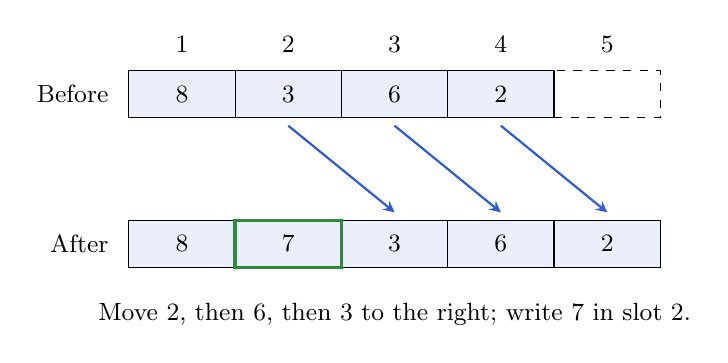
\begin{tikzpicture}[font=\small,>=stealth,x=1.35cm,y=1cm]
  \node[anchor=east] at (-0.6,0) {Before};
  \foreach \v [count=\i] in {8,3,6,2} {
    \draw[fill=PlotBlue!10] (\i-1.5,-0.3) rectangle (\i-0.5,0.3);
    \node at (\i-1,0) {$\v$};
    \node[above] at (\i-1,0.4) {$\i$};
  }
  \draw[dashed] (3.5,-0.3) rectangle (4.5,0.3);
  \node[above] at (4,0.4) {$5$};
  \node[anchor=east] at (-0.6,-1.9) {After};
  \foreach \v [count=\i] in {8,7,3,6,2} {
    \draw[fill=PlotBlue!10] (\i-1.5,-2.2) rectangle (\i-0.5,-1.6);
    \node at (\i-1,-1.9) {$\v$};
  }
  \draw[very thick,PlotGreen] (0.5,-2.2) rectangle (1.5,-1.6);
  \foreach \i in {1,2,3}
    \draw[->,PlotBlue,thick] (\i,-0.4) -- (\i+1,-1.5);
  \node[align=center] at (2,-2.8)
    {Move $2$, then $6$, then $3$ to the right; write $7$ in slot $2$.};
\end{tikzpicture}
\end{center}
Moving from right to left prevents overwriting a value before it
has been copied. We assume that one spare slot is available.
\end{framedexample}

  \item \listremoveop{i} takes $\Theta(n)$ time in the
    worst case: removing the first element shifts the remaining
    $n-1$ elements one place to the left.
\end{enumerate}

\Needspace{14\baselineskip}
\subsection{Linked lists: follow references}

\begin{frameddefn}{Singly linked list}\label{def:singly-linked-list}
A \emph{singly linked list} is a data structure that implements the
\hyperref[def:list-adt]{list ADT} using nodes. Each node contains an
element and a reference to the next node. A \emph{head} reference
identifies the first node; the last node has no successor.
\end{frameddefn}

\begin{framedexample}{A singly linked list}
The sequence $[8,3,6]$ is stored in three nodes.
\begin{center}
\begin{tikzpicture}[font=\small,>=stealth,
  cell/.style={draw,rounded corners,fill=PlotBlue!10,
    minimum width=1.4cm,minimum height=0.75cm}]
  \node (head) at (-1.8,0) {head};
  \node[cell] (a) at (0,0) {$8\mid\bullet$};
  \node[cell] (b) at (3.2,0) {$3\mid\bullet$};
  \node[cell] (c) at (6.4,0) {$6\mid\bullet$};
  \node (nil) at (8.5,0) {$\varnothing$};
  \draw[->,thick] (head) -- (a);
  \draw[->,thick] (a) -- node[above] {next} (b);
  \draw[->,thick] (b) -- node[above] {next} (c);
  \draw[->,thick] (c) -- (nil);
  \node[below=0.2cm of a] {position $1$};
  \node[below=0.2cm of b] {position $2$};
  \node[below=0.2cm of c] {position $3$};
  \node[align=center] at (3.2,-1.4)
    {The nodes need not occupy consecutive memory locations.};
\end{tikzpicture}
\end{center}
\end{framedexample}

To reach position $i$, we start at the head and follow $i-1$ links.

\begin{enumerate}
  \item \listgetop{i} takes $O(n)$ time in the worst case:
    follow the links to position $i$ and read the element. With a
    reference to the node already available, reading it takes
    $\Theta(1)$ time.
  \item \listsetop{x}{i} takes $O(n)$ time in the worst
    case: follow the links to position $i$ and replace the element
    with $x$. With a reference to the node already available, the
    replacement takes $\Theta(1)$ time.
  \item \listinsertop{x}{i} takes $O(n)$ time in the worst
    case: first find the node preceding position $i$. Once that
    reference is available, inserting the new node takes
    $\Theta(1)$ time. Inserting at the head also takes $\Theta(1)$ time.

\begin{framedexample}{Inserting after a known node}
Suppose we already have a reference to the node containing $8$.
To insert $7$ immediately after it, create a new node and update
two references:
\[
  \mathit{new.next}\gets\mathit{node8.next},\qquad
  \mathit{node8.next}\gets\mathit{new}.
\]
\begin{center}
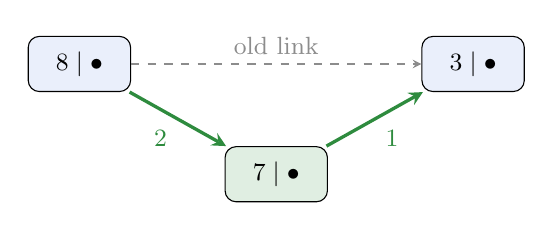
\begin{tikzpicture}[font=\small,>=stealth,
  cell/.style={draw,rounded corners,fill=PlotBlue!10,
    minimum width=1.3cm,minimum height=0.7cm}]
  \node[cell] (a) at (0,0) {$8\mid\bullet$};
  \node[cell] (b) at (5,0) {$3\mid\bullet$};
  \node[cell,fill=PlotGreen!15] (x) at (2.5,-1.4) {$7\mid\bullet$};
  \draw[->,dashed,black!45] (a) -- node[above] {old link} (b);
  \draw[->,very thick,PlotGreen] (x) -- node[below right] {$1$} (b);
  \draw[->,very thick,PlotGreen] (a) -- node[below left] {$2$} (x);
\end{tikzpicture}
\end{center}
The update takes $\Theta(1)$ time. If we were only given an index,
we would first have to find the preceding node.
\end{framedexample}

  \item \listremoveop{i} takes $O(n)$ time in the worst
    case: first find the node preceding position $i$. With that
    reference available, bypass the removed node by changing the
    predecessor's \texttt{next} link in $\Theta(1)$ time. Removing
    the head takes $\Theta(1)$ time: update the head reference.
\end{enumerate}

\Needspace{15\baselineskip}
\subsection{Doubly linked lists and operation costs}

\begin{frameddefn}{Doubly linked list}\label{def:doubly-linked-list}
A \emph{doubly linked list} is a data structure that implements the
\hyperref[def:list-adt]{list ADT} using nodes. Each node contains an
element, a \texttt{next} reference to its successor, and a
\texttt{previous} reference to its predecessor, when these exist.
\end{frameddefn}

From a node, we can directly reach both neighbours.
Finding a node by its index still requires following links.

\begin{framedexample}{A doubly linked list}
The sequence $[8,3,6]$ has links in both directions between adjacent nodes.
\begin{center}
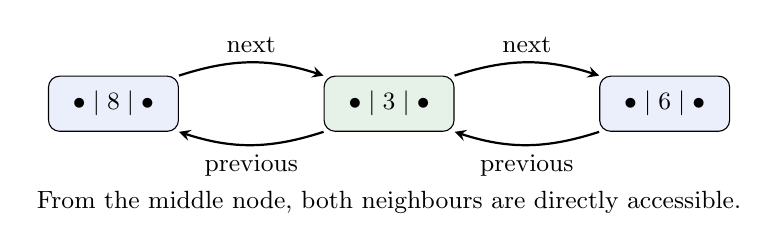
\begin{tikzpicture}[font=\small,>=stealth,
  cell/.style={draw,rounded corners,fill=PlotBlue!10,
    minimum width=1.65cm,minimum height=0.7cm}]
  \node[cell] (a) at (0,0) {$\bullet\mid8\mid\bullet$};
  \node[cell,fill=PlotGreen!12] (b) at (3.5,0) {$\bullet\mid3\mid\bullet$};
  \node[cell] (c) at (7,0) {$\bullet\mid6\mid\bullet$};
  \draw[->,thick] (a.north east) to[bend left=18]
    node[above] {next} (b.north west);
  \draw[->,thick] (b.south west) to[bend left=18]
    node[below] {previous} (a.south east);
  \draw[->,thick] (b.north east) to[bend left=18]
    node[above] {next} (c.north west);
  \draw[->,thick] (c.south west) to[bend left=18]
    node[below] {previous} (b.south east);
  \node[align=center] at (3.5,-1.25)
    {From the middle node, both neighbours are directly accessible.};
\end{tikzpicture}
\end{center}
\end{framedexample}

\begin{enumerate}
  \item \listgetop{i} takes $O(n)$ time in the worst case
    to locate position $i$. Reading the element of a node whose
    reference is already available takes $\Theta(1)$ time.
  \item \listsetop{x}{i} takes $O(n)$ time in the worst
    case to locate position $i$. Replacing the element of a known
    node takes $\Theta(1)$ time.
  \item \listinsertop{x}{i} takes $O(n)$ time in the worst
    case to locate the insertion position. Given a reference to the
    adjacent node, linking in the new node takes $\Theta(1)$ time:
    update the neighbours' \texttt{next} and \texttt{previous}
    references, and the head or tail if necessary.
  \item \listremoveop{i} takes $O(n)$ time in the worst
    case to locate position $i$. Given a reference to that node,
    unlinking it takes $\Theta(1)$ time: its \texttt{previous}
    reference gives direct access to its predecessor. Update the
    neighbours' links and the head or tail if necessary.
\end{enumerate}

The following table concerns the \emph{indexed operations of the
list ADT}. Bounds are worst-case bounds for a list of $n$ elements;
array insertion assumes available capacity.
\begin{center}
\small
\begin{tabular}{lcccc}
\hline
Data structure & \listgetop{i} & \listsetop{x}{i} & \listinsertop{x}{i} & \listremoveop{i} \\[3pt]
\hline
Array & $\Theta(1)$ & $\Theta(1)$ & $O(n)$ & $O(n)$ \\
Singly linked & $O(n)$ & $O(n)$ & $O(n)$ & $O(n)$ \\
Doubly linked & $O(n)$ & $O(n)$ & $O(n)$ & $O(n)$ \\
\hline
\end{tabular}
\end{center}

The advantage of linked lists appears when the needed references
are already available: inserting after a known node is constant
time, and a doubly linked list also removes a known node in constant
time. These are different requests from finding and removing
\emph{the element at index $i$}.

\section{The priority queue ADT}

For top-$k$ selection, positions in a sequence are not our main
concern. We repeatedly need the candidate with an extreme score.
A priority queue provides operations tailored to that task.

\begin{frameddefn}{Max-priority queue (ADT)}\label{def:max-priority-queue}
A \emph{max-priority queue} stores entries with comparable
priorities and supports:
\begin{enumerate}
  \item \pqinsertop{x}: add entry $x$;
  \item \pqpeekop{Max}: return an entry of maximum
    priority without removing it;
  \item \pqextractop{Max}: remove and return an entry
    of maximum priority.
\end{enumerate}
The last two operations require a nonempty queue. Equal priorities
are allowed. For a queue of numbers, each number is its own priority.
\end{frameddefn}

\begin{frameddefn}{Min-priority queue (ADT)}\label{def:min-priority-queue}
A \emph{min-priority queue} stores entries with comparable priorities
and supports:
\begin{enumerate}
  \item \pqinsertop{x}: add entry $x$;
  \item \pqpeekop{Min}: return an entry of minimum priority
    without removing it;
  \item \pqextractop{Min}: remove and return an entry of
    minimum priority.
\end{enumerate}
The last two operations require a nonempty queue. Equal priorities
are allowed. For a queue of numbers, each number is its own priority.
\end{frameddefn}

The ADT specifies the result of each operation; it does not require
a particular representation.

We now consider two data structures that can implement the
\hyperref[def:max-priority-queue]{max-priority queue ADT}: an unsorted
array and a sorted array. Both support the same three operations,
but their representation changes the cost of each operation.

\textbf{An unsorted array.}
Insertion at the end is cheap, but finding the maximum requires a
scan. Once found, it can be removed by replacing it with the last
entry: a priority queue does not have to preserve sequence order.
The scan still makes extraction linear.

\textbf{A sorted array.}
If the array is in increasing order, the maximum is the last entry.
Reading or removing it is constant time, but inserting a new entry
in sorted order may require shifting $\Theta(n)$ entries.

Can we do better than this for our use case?

We would like fast access to the maximum \emph{and} fast updates.
A binary heap provides that compromise.

\section{Binary heaps}

For the numerical heaps considered here, each node's value is its priority.

\begin{frameddefn}{Binary max-heap}\label{def:binary-max-heap}
A \emph{binary max-heap} is a data structure that implements the
\hyperref[def:max-priority-queue]{max-priority queue ADT}. It is
represented as a binary tree satisfying two conditions:
\begin{enumerate}
  \item \textbf{Shape:} every level is full except possibly the last,
    which is filled from left to right. Such a tree is
    \emph{complete}.
  \item \textbf{Order:} each parent's value is greater than or
    equal to the values of its children.
\end{enumerate}
\end{frameddefn}

\begin{frameddefn}{Binary min-heap}\label{def:binary-min-heap}
A \emph{binary min-heap} is a data structure that implements the
\hyperref[def:min-priority-queue]{min-priority queue ADT}. It is
represented as a binary tree satisfying two conditions:
\begin{enumerate}
  \item \textbf{Shape:} every level is full except possibly the last,
    which is filled from left to right. Such a tree is
    \emph{complete}.
  \item \textbf{Order:} each parent's value is less than or
    equal to the values of its children.
\end{enumerate}
\end{frameddefn}

In a max-heap, following a path from the root downwards never
increases the value. Therefore the root contains a global maximum, and
$\pqpeekop{Max}$ takes $\Theta(1)$ time.

In a min-heap, values never decrease along a path from the root
downwards. The root therefore contains a global minimum, and
$\pqpeekop{Min}$ takes $\Theta(1)$ time.

\begin{framedexample}{A max-heap and its array}\label{ex:heap-array}
The small labels give positions in \emph{level order}: read each
level from left to right, starting at the root.
\begin{center}
\begin{tikzpicture}[font=\small,>=stealth,
  heapnode/.style={circle,draw,fill=PlotBlue!12,minimum size=0.7cm,
    inner sep=1pt}]
  \foreach \i/\v/\x/\y in {
    1/20/0/0,2/12/-3/-1.2,3/16/3/-1.2,
    4/7/-4.5/-2.4,5/8/-1.5/-2.4,6/9/1.5/-2.4,7/4/4.5/-2.4,
    8/1/-5.2/-3.6,9/5/-3.8/-3.6,10/2/-2.2/-3.6,
    11/6/-0.8/-3.6,12/3/0.8/-3.6} {
    \node[heapnode] (h\i) at (\x,\y) {$\v$};
    \node[font=\scriptsize,anchor=south west,text=black!65]
      at (h\i.north east) {$\i$};
  }
  \foreach \p/\c in {1/2,1/3,2/4,2/5,3/6,3/7,4/8,4/9,5/10,5/11,6/12}
    \draw (h\p) -- (h\c);
  \node[above=0.25cm of h1,text=PlotGreen!60!black]
    {maximum at the root};
  \foreach \v [count=\i] in {20,12,16,7,8,9,4,1,5,2,6,3} {
    \draw[fill=PlotBlue!10] ({(\i-6.5)*0.88-0.44},-5.3)
      rectangle ({(\i-6.5)*0.88+0.44},-4.7);
    \node at ({(\i-6.5)*0.88},-5) {$\v$};
    \node[font=\scriptsize] at ({(\i-6.5)*0.88},-5.6) {$\i$};
  }
\end{tikzpicture}
\end{center}
For example, $12\geq7,8$ and $16\geq9,4$. The last level is
filled on the left. The next inserted node occupies position $13$,
the right child of position $6$.
\end{framedexample}

Because the shape has no gaps, we can store a heap in an array
$H[1],\ldots,H[n]$, as in Example~\ref{ex:heap-array}.

\subsection{Store the tree in an array}

With \emph{one-based indexing}, the links are implicit:
\[
  \operatorname{parent}(i)=\left\lfloor\frac{i}{2}\right\rfloor
  \quad(i>1),\qquad
  \operatorname{left}(i)=2i,\qquad
  \operatorname{right}(i)=2i+1.
\]
A child exists only when its index is at most $n$.
For example, node $5$ has children $10$ and $11$; node $6$ has
child $12$, but no child $13$ yet. We calculate these positions
without storing explicit pointer fields.

At depth $d$, a full level has $2^d$ nodes. A complete tree with
$n\geq1$ nodes has height $\lfloor\log_2 n\rfloor$, counting
edges from the root to the deepest leaf. A path up or down therefore
contains only $O(\log n)$ edges for $n\geq2$.

\subsection{Insertion: move up until the order is restored}

How do we insert a value in the heap while preserving the structure?

First append the new entry in the next free array slot. This
preserves completeness, but its value might exceed its parent's.
While that happens, swap the two and continue from the parent.
This operation is called \emph{sift-up}.

Only the new entry's path to the root can violate the order. Each
swap moves it one level up, so there are at most $O(\log n)$ swaps.

\begin{framedexample}{Insert $18$ into a smaller max-heap}\label{ex:heap-insert-eighteen}
Start with $H=[20,12,16,7,8,9,4]$. Append $18$ at position $8$.
Its path to the root is $8\to4\to2\to1$.
\begin{center}
\small
\begin{tabular}{ll}
\hline
Action & Array \\
\hline
Append $18$ & $[20,12,16,7,8,9,4,\mathbf{18}]$ \\
Swap with $7$ & $[20,12,16,\mathbf{18},8,9,4,7]$ \\
Swap with $12$ & $[20,\mathbf{18},16,12,8,9,4,7]$ \\
Stop: $18\leq20$ & $[20,18,16,12,8,9,4,7]$ \\
\hline
\end{tabular}
\end{center}
Both drawings show the entire heap. Green arrows show how $18$ moves up.
\begin{center}
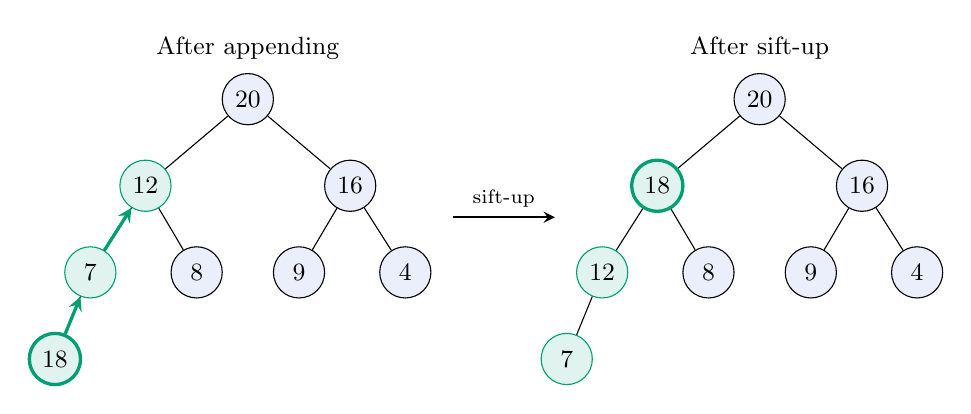
\begin{tikzpicture}[font=\small,>=stealth,
  hn/.style={circle,draw,fill=PlotBlue!10,minimum size=0.65cm,inner sep=1pt},
  unchanged/.style={},
  moved/.style={draw=ListInsert,fill=ListInsert!12},
  inserted/.style={moved,very thick}]
  \foreach \side/\shift in {a/0,b/6.5} {
    \begin{scope}[xshift=\shift cm]
      \foreach \i/\x/\y in {1/0/0,2/-1.3/-1.1,3/1.3/-1.1,
          4/-2/-2.2,5/-0.65/-2.2,6/0.65/-2.2,7/2/-2.2,
          8/-2.45/-3.3}
        \coordinate (\side p\i) at (\x,\y);
    \end{scope}
  }
  \foreach \i/\v/\kind in {1/20/unchanged,2/12/moved,3/16/unchanged,
      4/7/moved,5/8/unchanged,6/9/unchanged,7/4/unchanged,8/18/inserted}
    \node[hn,\kind] (a\i) at (ap\i) {$\v$};
  \foreach \i/\v/\kind in {1/20/unchanged,2/18/inserted,3/16/unchanged,
      4/12/moved,5/8/unchanged,6/9/unchanged,7/4/unchanged,8/7/moved}
    \node[hn,\kind] (b\i) at (bp\i) {$\v$};
  \foreach \p/\c in {1/2,1/3,2/4,2/5,3/6,3/7,4/8} {
    \draw (a\p) -- (a\c);
    \draw (b\p) -- (b\c);
  }
  \draw[->,very thick,ListInsert] (a8) -- (a4);
  \draw[->,very thick,ListInsert] (a4) -- (a2);
  \draw[->,thick] (2.6,-1.5) -- node[above,font=\scriptsize] {sift-up}
    (3.9,-1.5);
  \node at (0,0.65) {After appending};
  \node at (6.5,0.65) {After sift-up};
\end{tikzpicture}
\end{center}
The root remains $20$. Insertion rearranges the path without
sorting the whole array.
\end{framedexample}

The heap repair costs $O(\log n)$ in the worst case. With an
array of sufficient capacity, this is also the insertion cost.
With a dynamic array that occasionally resizes, the overall
insertion bound is $O(\log n)$ amortized for $n\geq2$; a resizing
insertion can itself take $\Theta(n)$ time.

\subsection{Extraction: replace the root and move down}

To extract the maximum:
\begin{enumerate}
  \item Save the root's entry to return it.
  \item Move the last entry to the root and reduce the heap size by
    one. If the heap is now empty, stop.
  \item If the entry is smaller than a child, swap it with its
    \emph{larger} child. Continue downwards until the order is restored.
\end{enumerate}
This repair is called \emph{sift-down}. Choosing the larger child
makes the new parent at least as large as both children. The
possible violation moves down one path, which has logarithmic length.

\begin{framedexample}{Extract $20$ after the insertion}
The heap from the previous example is
$[20,18,16,12,8,9,4,7]$. Save $20$ and put the last entry, $7$,
at the root. Position $8$ is no longer in the heap.
\begin{center}
\small
\begin{tabular}{ll}
\hline
Action & Array \\
\hline
Replace root with $7$ & $[\mathbf{7},18,16,12,8,9,4]$ \\
Swap with $18$ & $[18,\mathbf{7},16,12,8,9,4]$ \\
Swap with $12$ & $[18,12,16,\mathbf{7},8,9,4]$ \\
Stop at a leaf & $[18,12,16,7,8,9,4]$ \\
\hline
\end{tabular}
\end{center}
\begin{center}
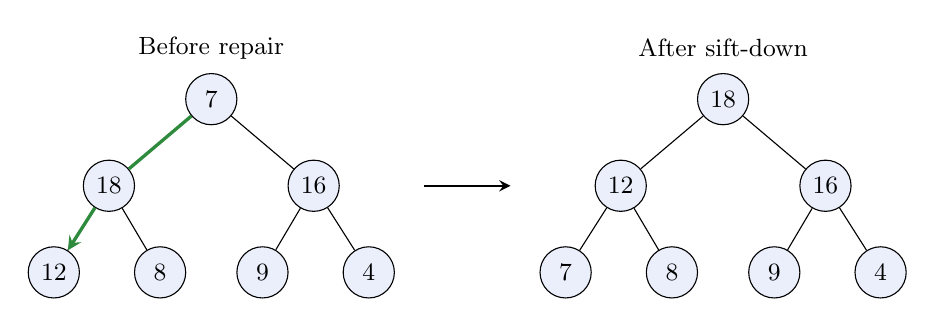
\begin{tikzpicture}[font=\small,>=stealth,
  hn/.style={circle,draw,fill=PlotBlue!10,minimum size=0.65cm,inner sep=1pt}]
  \foreach \side/\shift in {a/0,b/6.5} {
    \begin{scope}[xshift=\shift cm]
      \foreach \i/\x/\y in {1/0/0,2/-1.3/-1.1,3/1.3/-1.1,
          4/-2/-2.2,5/-0.65/-2.2,6/0.65/-2.2,7/2/-2.2}
        \coordinate (\side p\i) at (\x,\y);
    \end{scope}
  }
  \foreach \i/\v in {1/7,2/18,3/16,4/12,5/8,6/9,7/4}
    \node[hn] (a\i) at (ap\i) {$\v$};
  \foreach \i/\v in {1/18,2/12,3/16,4/7,5/8,6/9,7/4}
    \node[hn] (b\i) at (bp\i) {$\v$};
  \foreach \p/\c in {1/2,1/3,2/4,2/5,3/6,3/7} {
    \draw (a\p) -- (a\c);
    \draw (b\p) -- (b\c);
  }
  \node at (0,0.65) {Before repair};
  \node at (6.5,0.65) {After sift-down};
  \draw[->,very thick,PlotGreen] (a1) -- (a2) -- (a4);
  \draw[->,thick] (2.7,-1.1) -- (3.8,-1.1);
\end{tikzpicture}
\end{center}
At the first step, choose $18$ rather than $16$. At the second,
choose $12$ rather than $8$. The returned entry is $20$; the new
maximum is $18$.
\end{framedexample}

Extraction takes $O(\log n)$ time in the worst case, assuming
removing the final array slot does not trigger resizing.
Reading the maximum alone requires no repair and remains
$\Theta(1)$.

\subsection{Comparing priority queue implementations}

For a queue containing $n\geq2$ entries, the following bounds
assume arrays have sufficient capacity and removal does not resize
them. The sorted array keeps its maximum at the last occupied slot.
\begin{center}
\small
\begin{tabular}{lccc}
\hline
Representation & \pqinsertop{x} & \pqpeekop{Max} & \pqextractop{Max} \\[3pt]
\hline
Unsorted array & $\Theta(1)$ & $\Theta(n)$ & $\Theta(n)$ \\
Sorted array   & $O(n)$ & $\Theta(1)$ & $\Theta(1)$ \\
Binary max-heap & $O(\log n)$ & $\Theta(1)$ & $O(\log n)$ \\
\hline
\end{tabular}
\end{center}

The heap keeps enough order to expose the maximum, without paying
to keep every entry in sorted order after each insertion.

\section{Sorting with a heap}\label{sec:heapsort}

A max-heap gives us the largest remaining value at every
extraction. Can we use this operation to sort an entire array?
We first use a separate output array, then see how to reuse the
input array itself.

\subsection{Sorting into a second array}

Let $A[1],\ldots,A[n]$ be the input. First turn $A$ into a
max-heap, using its own storage. One way to do this with the
operations we already know is to grow a heap one entry at a time:
for $j=2,\ldots,n$, regard $A[j]$ as the newly appended entry
and sift it up inside $A[1],\ldots,A[j]$. The later entries
are untouched. We call this procedure
$\operatorname{BuildMaxHeapByInsertion}(A)$; it takes
$O(n\log n)$ time and can be implemented with a loop using
$O(1)$ extra working space.

Once the max-heap is ready, allocate a second array $B$ of size $n$.
For $n\geq1$, fill it as follows:
\begin{enumerate}
  \item For $j=n,n-1,\ldots,2$, extract the maximum, repairing
    the remaining heap by sifting down, and store the extracted value in $B[j]$.
  \item Copy the only remaining value into $B[1]$.
\end{enumerate}
The largest value goes into the last position, the next largest
into the preceding position, and so on: $B[1]\leq\cdots\leq B[n]$.
There are $n-1$ extractions; the last value needs no repair.
An empty input is already sorted.

\begin{framedexample}{Fill the output array from right to left}
Reuse the seven-entry heap from the start of
Example~\ref{ex:heap-insert-eighteen}, before inserting $18$:
\[
H=[20,12,16,7,8,9,4].
\]
Each row below shows $B$ after storing one value.
The symbol $\square$ denotes an output cell that has not yet been filled.
\begin{center}
\small
\begin{tabular}{ll}
\hline
Action & Output array $B$ \\
\hline
Extract $20$ & $[\square,\square,\square,\square,\square,\square,20]$ \\
Extract $16$ & $[\square,\square,\square,\square,\square,16,20]$ \\
Extract $12$ & $[\square,\square,\square,\square,12,16,20]$ \\
Extract $9$  & $[\square,\square,\square,9,12,16,20]$ \\
Extract $8$  & $[\square,\square,8,9,12,16,20]$ \\
Extract $7$  & $[\square,7,8,9,12,16,20]$ \\
Copy $4$    & $[4,7,8,9,12,16,20]$ \\
\hline
\end{tabular}
\end{center}
The six extractions return values in decreasing order; placing
them from right to left produces an increasing array.
\end{framedexample}

Building the heap takes $O(n\log n)$ time with the method above.
The $n-1$ extractions take another $O(n\log n)$ time in total,
so the overall bound is $O(n\log n)$. The second array uses
$\Theta(n)$ additional space.

\subsection{Reuse the input array: in-place HeapSort}

Can we avoid allocating a second array? Each extraction reduces
the active heap size by one. We can store the extracted maximum
in the cell that has just left the heap.

\begin{frameddefn}{In-place sorting}
An \emph{in-place sorting algorithm} rearranges the entries in
the input array using $O(1)$ additional working space.
The storage occupied by the input array itself is not counted
as additional space.
\end{frameddefn}

Suppose the active heap occupies $A[1],\ldots,A[m]$.
Instead of removing its root and allocating space elsewhere:
\begin{enumerate}
  \item Swap $A[1]$ with $A[m]$. The maximum is now in its final
    position, $m$.
  \item Reduce the active heap size to $m-1$. The physical array
    still contains $n$ cells.
  \item Sift down the new root, considering only positions
    $1,\ldots,m-1$. The sorted suffix must stay outside the repair.
\end{enumerate}
Repeat for $m=n,n-1,\ldots,2$. This is \emph{HeapSort}:
the heap shrinks on the left while the sorted suffix grows on the right.

\begin{framedexample}{HeapSort in the same array}
Start from the same heap $[20,12,16,7,8,9,4]$.
In the first pass, swap $20$ with $4$:
\[
[\underbrace{4,12,16,7,8,9}_{\text{repair this prefix}}\mid20].
\]
Sift-down swaps $4$ with $16$, then with $9$, giving
$[16,12,9,7,8,4\mid20]$.

Below, every row after the first shows the \emph{completed repair}
of one pass. All seven cells belong to the same array throughout.
\begin{center}
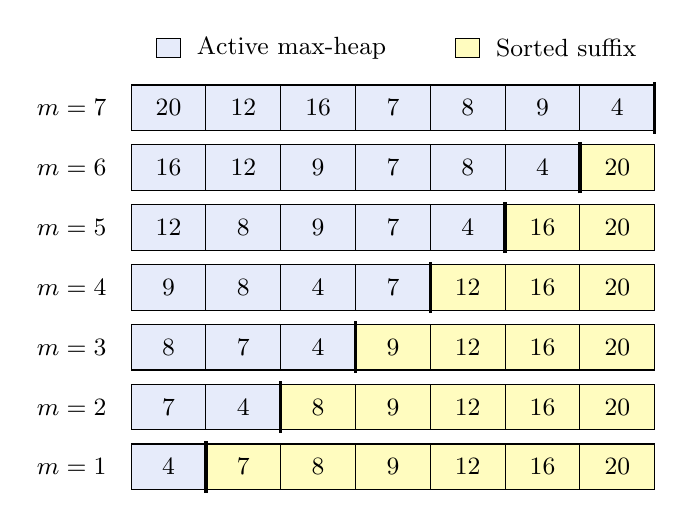
\begin{tikzpicture}[x=0.95cm,y=0.76cm,
  cell/.style={draw,minimum width=0.95cm,minimum height=0.58cm,
    inner sep=0pt,font=\small}]
  \node[draw,fill=PlotBlue!12,minimum width=0.3cm,minimum height=0.25cm]
    at (0,1) {};
  \node[anchor=west,font=\small] at (0.25,1) {Active max-heap};
  \node[draw,fill=yellow!25,minimum width=0.3cm,minimum height=0.25cm]
    at (4,1) {};
  \node[anchor=west,font=\small] at (4.25,1) {Sorted suffix};
  \foreach \r/\m/\vals in {
    0/7/{20,12,16,7,8,9,4},
    1/6/{16,12,9,7,8,4,20},
    2/5/{12,8,9,7,4,16,20},
    3/4/{9,8,4,7,12,16,20},
    4/3/{8,7,4,9,12,16,20},
    5/2/{7,4,8,9,12,16,20},
    6/1/{4,7,8,9,12,16,20}} {
    \node[anchor=east,font=\small] at (-0.7,-\r) {$m=\m$};
    \foreach \v [count=\i from 1] in \vals {
      \ifnum\i>\m
        \node[cell,fill=yellow!25] at (\i-1,-\r) {$\v$};
      \else
        \node[cell,fill=PlotBlue!12] at (\i-1,-\r) {$\v$};
      \fi
    }
    \draw[very thick] (\m-0.5,-\r-0.43) -- (\m-0.5,-\r+0.43);
  }
\end{tikzpicture}
\end{center}
At $m=1$, the remaining heap consists only of the minimum, $4$.
The entire array is now sorted; no further extraction is needed.
\end{framedexample}

\begin{framedalgo}{In-place HeapSort}\label{alg:heapsort}
\begin{algorithmic}[1]
  \Function{HeapSort}{$A$}
    \State $n\gets\operatorname{length}(A)$
    \If{$n\leq1$}
      \State \Return $A$
    \EndIf
    \State \Call{BuildMaxHeapByInsertion}{$A$}
    \For{$m=n,n-1,\ldots,2$}
      \State swap $A[1]$ and $A[m]$
      \State \Call{SiftDownPrefix}{$A,1,m-1$}
    \EndFor
    \State \Return $A$
  \EndFunction
\end{algorithmic}
\end{framedalgo}

Here $\operatorname{SiftDownPrefix}(A,i,m)$ repairs the heap
starting at position $i$, using only the first $m$ cells.
Its children must already root valid max-heaps, as they do after
the root swap in HeapSort. An iterative implementation makes
the space bound explicit:

\begin{framedalgo}{Sift down inside the active prefix}
\begin{algorithmic}[1]
  \Function{SiftDownPrefix}{$A,i,m$}
    \While{$2i\leq m$}
      \State $j\gets2i$ \Comment{left child exists}
      \If{$j<m$} \Comment{right child also exists}
        \If{$A[j+1]>A[j]$}
          \State $j\gets j+1$
        \EndIf
      \EndIf
      \If{$A[i]\geq A[j]$}
        \State \Return
      \EndIf
      \State swap $A[i]$ and $A[j]$
      \State $i\gets j$
    \EndWhile
  \EndFunction
\end{algorithmic}
\end{framedalgo}

\textbf{Why it works.}
At the start of a pass with active size $m$:
\begin{enumerate}
  \item $A[1],\ldots,A[m]$ form a max-heap.
  \item $A[m+1],\ldots,A[n]$ are in increasing order.
  \item Every value in the heap is less than or equal to every
    value in the sorted suffix, when that suffix is nonempty.
\end{enumerate}
The root is the largest remaining value. Moving it to position
$m$ extends the sorted suffix by one cell. Sift-down restores
the heap in the smaller prefix without touching that suffix.
When only one heap entry remains, these properties imply that
the entire array is sorted. Equal values cause no difficulty.

\textbf{Time and space.}
With the insertion-based construction described above, building
the heap costs $O(n\log n)$. The sorting passes cost
\[
  \sum_{m=2}^{n}O(\log m)\;=\;O(n\log n).
\]
Thus HeapSort takes $O(n\log n)$ time in the worst case.
Using iterative sift-up and sift-down, it needs only a constant
number of indices and a temporary value for swaps: $O(1)$ extra
working space. The second array $B$ is no longer needed.

\section{Use a heap to select the top k}\label{sec:heap-top-k}

We can now complete the selection step introduced in
Section~\ref{sec:vector-search}. To keep the $k$ \emph{largest}
scores, we repeatedly need the \emph{smallest retained score}:
it is the weakest candidate and the one a better entry replaces.

We therefore use a \emph{min-heap} of at most $k$ entries
(Definition~\ref{def:binary-min-heap}). Its array representation
is the same as for a max-heap. Insertions sift up when a child
is smaller than its parent; extraction sifts down using the smaller
child. The operation bounds are unchanged.

\begin{notebox}[Which heap should we use?]
To keep the $k$ largest values, use a \textbf{min-heap}: its root
is the smallest value currently retained, so it is the candidate
to replace when a larger value arrives.

To keep the $k$ smallest values, use a \textbf{max-heap}: its root
is the largest value currently retained, so it is the candidate
to replace when a smaller value arrives.
\end{notebox}

The root should expose the retained candidate that we would discard
first. It is not necessarily the best result we eventually return.

\begin{framedalgo}{Keep the $k$ largest scores}\label{alg:heap-top-k}
\begin{algorithmic}[1]
  \Function{TopKWithHeap}{$A,k$}
    \State $Q\gets$ an empty min-priority queue with capacity $k$
    \For{each entry $x$ in $A$}
      \If{$\operatorname{size}(Q)<k$}
        \State $Q.\pqinsertop{x}$
      \ElsIf{$x>Q.\pqpeekop{Min}$}
        \State $Q.\pqextractop{Min}$
        \State $Q.\pqinsertop{x}$
      \EndIf
    \EndFor
    \State \Return the entries stored in $Q$
  \EndFunction
\end{algorithmic}
\end{framedalgo}

\textbf{Why it works.}
After processing $t$ entries, $Q$ contains the largest $\min(k,t)$
scores seen so far, allowing any choice among tied entries.
Until it fills, it keeps every entry. Afterwards, let $m$ be its
minimum. A new score $x\leq m$ cannot improve the retained scores;
a score $x>m$ must replace one occurrence of $m$. Both cases
preserve the claim. At $t=n$, it gives exactly the required result.

\begin{framedexample}{Follow the top-$3$ candidates}\label{ex:heap-top-three}
Process the scores from our opening example. Arrays below are
valid min-heap representations; they are not sorted lists.
\begin{center}
\small
\begin{tabular}{cll}
\hline
New score & Action & Heap array afterwards \\
\hline
$12$ & Insert & $[12]$ \\
$7$  & Insert and sift up & $[7,12]$ \\
$20$ & Insert & $[7,12,20]$ \\
$3$  & Discard: $3\leq7$ & $[7,12,20]$ \\
$16$ & Replace $7$ & $[12,20,16]$ \\
$9$  & Discard: $9\leq12$ & $[12,20,16]$ \\
$25$ & Replace $12$ & $[16,20,25]$ \\
\hline
\end{tabular}
\end{center}
The three full heaps at the replacement steps are:
\begin{center}
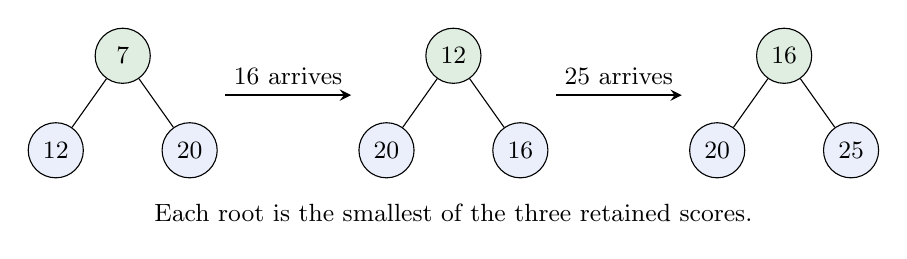
\begin{tikzpicture}[font=\small,>=stealth,
  hn/.style={circle,draw,fill=PlotBlue!10,minimum size=0.7cm,inner sep=1pt}]
  \foreach \name/\shift/\root/\lv/\rv in
      {a/0/7/12/20,b/4.2/12/20/16,c/8.4/16/20/25} {
    \node[hn,fill=PlotGreen!15] (\name r) at (\shift,0) {$\root$};
    \node[hn] (\name l) at (\shift-0.85,-1.2) {$\lv$};
    \node[hn] (\name q) at (\shift+0.85,-1.2) {$\rv$};
    \draw (\name r) -- (\name l);
    \draw (\name r) -- (\name q);
  }
  \draw[->,thick] (1.3,-0.5) -- node[above] {$16$ arrives} (2.9,-0.5);
  \draw[->,thick] (5.5,-0.5) -- node[above] {$25$ arrives} (7.1,-0.5);
  \node[align=center] at (4.2,-2)
    {Each root is the smallest of the three retained scores.};
\end{tikzpicture}
\end{center}
The final candidates have scores $16,20,25$. If the search engine
must display them in decreasing score order, sort just these three.
\end{framedexample}

\subsection{Time, space and the search-engine connection}

Each score requires a constant-time size or root check. If retained,
it causes at most one extraction and one insertion on a heap of
size at most $k$. Thus the total selection cost is
\[
  O\bigl(n\log(k+1)\bigr),
  \qquad\text{with }O(k)\text{ additional space}.
\]
For $k\geq2$, we usually write this as $O(n\log k)$.
Writing $\log(k+1)$ also covers $k=1$: keeping a single maximum
requires one linear scan, not zero work.
Capacity $k$ can be allocated once; no heap growth beyond that
capacity is needed. If an ordered output is required, sorting the
$k$ retained entries adds $O(k\log k)$ time.

For example, with $n=10^6$ and $k=10$, heap updates traverse a
tree of height at most $\lfloor\log_2 10\rfloor=3$, rather than
ordering a million scores. Every input score is still examined.

In Algorithm~\ref{alg:ranked-index}, the inverted index reduces
the work needed to \emph{compute} the scores. The heap improves the
subsequent step that \emph{selects} the best results. If $c$ candidate
documents receive scores, replacing their full sort with a heap
changes that selection cost from $O(c\log c)$ to
$O(c\log(k+1))$, for $1\leq k\leq c$. We still need to compute
each candidate's complete score before comparing it with the heap
root. If fewer than $k$ candidates are available, return all of them.

\endgroup

\end{document}
